% !TEX program = lualatex
% !TEX option = -outdir=output
\documentclass[openany]{book}
\usepackage{subcaption}
\usepackage{graphicx} % Required for inserting images
\usepackage[fontset=none]{ctex}        % 明确禁用自动字体集
\usepackage{fontspec}
% 手动指定 macOS 系统字体（常用名称）
\setCJKmainfont{Songti SC}             % 或 STSongSC-Light
\setCJKsansfont{Heiti SC}              % 或 STHeitiSC-Light
\setCJKmonofont{Kaiti SC}              % 或 STKaitiSC-Light
\usepackage{amsmath}
\usepackage{amssymb}
\usepackage{bm}
\usepackage{physics}
\usepackage{geometry}
\geometry{left=2.5cm, right=2.5cm, top=2.5cm, bottom=2.5cm}
\usepackage{enumitem}
\usepackage{hyperref}
\usepackage{fontspec}
\usepackage{unicode-math}
% 设置主字体为 STIX Two Text
\setmainfont{STIXTwoText}[
    Extension = .otf,
    UprightFont = *-Regular,
    BoldFont = *-Bold,
    ItalicFont = *-Italic,
    BoldItalicFont = *-BoldItalic,
]
\setmathfont{STIX Two Math}
\setmathfont{STIX Two Math}[StylisticSet=1,range={scr,bfscr}]

\usepackage{esint}
\usepackage{tikz}
\usetikzlibrary{
    arrows.meta,    % 美观的箭头样式
    angles,         % 角度标注
    quotes,         % 角度标签美化
    calc            % 坐标计算
}
% 导入需要的TikZ库：路径变形（画弹簧）、计算（坐标运算）
\usetikzlibrary{decorations.pathmorphing,calc}
% Lagrangian
\newcommand{\Lag}{\mathscr{L}}
% 算符
\newcommand{\de}[2]{\frac{\dd{#1}}{\dd{#2}}}
\newcommand{\dde}[2]{\frac{\dd^2{#1}}{\dd{#2}^2}}
\newcommand{\dt}[1]{\frac{\mathrm{d} #1}{\mathrm{d}t}}
\newcommand{\pd}[2]{\frac{\partial{#1}}{\partial{#2}}}
\newcommand{\pdd}[2]{\frac{\partial^{2} #1}{\partial{#2}^{2}}}
\newcommand{\mpd}[3]{\frac{\partial^2 #1}{\partial{#2} \partial{#3}}}
\newcommand{\dOmega}[1]{\frac{\mathrm{d}{#1}}{\mathrm{d}\Omega}}
\newcommand{\pdt}{\partial_{t}}
\newcommand{\Ham}{\hat{H}}
\newcommand{\avg}[1]{\left\langle{#1}\right\rangle}
\newcommand{\br}[1]{\left({#1}\right)}
\newcommand{\mbr}[1]{\left[{#1}\right]} 
\newcommand{\bbr}[1]{\left\{{#1}\right\}}
\newcommand{\evalat}[2]{\left.{#1}\right|_{#2}}
% 坐标与矢量
\newcommand{\dq}{\dot{q}}
\newcommand{\ddq}{\ddot{q}}
\newcommand{\vq}{\mathbf{q}}
\newcommand{\const}{\mathrm{const}}
\newcommand{\vr}{\mathbf{x}}
\newcommand{\vp}{\mathbf{p}}
\newcommand{\vk}{\mathbf{k}}
\newcommand{\vj}{\mathbf{j}}
\newcommand{\vL}{\mathbf{L}}
\newcommand{\vS}{\mathbf{S}}
\newcommand{\vJ}{\mathbf{J}}
\newcommand{\uv}[1]{\hat{\symbf{#1}}}
% 瞬时物理场（实数）
\newcommand{\vEr}{\vec{\mathcal{E}}}
\newcommand{\vHr}{\vec{\mathcal{H}}}
\newcommand{\vBr}{\vec{\mathcal{B}}}
\newcommand{\vDr}{\vec{\mathcal{D}}}
\newcommand{\vPr}{\vec{\mathcal{P}}}
\newcommand{\vMr}{\vec{\mathcal{M}}}
\newcommand{\Er}{\mathcal{E}}
\newcommand{\Hr}{\mathcal{H}}
\newcommand{\Br}{\mathcal{B}}
\newcommand{\Dr}{\mathcal{D}}
\newcommand{\cPr}{\mathcal{P}}
\newcommand{\cMr}{\mathcal{M}}
% 复振幅(复数)
\newcommand{\vE}{\mathbf{E}}
\newcommand{\vH}{\mathbf{H}}
\newcommand{\vB}{\mathbf{B}}
\newcommand{\vD}{\mathbf{D}}
\newcommand{\vP}{\mathbf{P}}
\newcommand{\vM}{\mathbf{M}}
\newcommand{\vA}{\mathbf{A}}
% 约化质量
\newcommand{\mr}{m_{\mu}}
% 快速表示
\newcommand{\eff}{\mathrm{eff}}
\newcommand{\ret}{\mathrm{ret}}
\newcommand{\rad}{\mathrm{rad}}
\newcommand{\hh}{\hbar}
\newcommand{\psit}{\psi(t)}
\newcommand{\up}{\uparrow}
\newcommand{\down}{\downarrow}
\newcommand{\lscr}{\mathcal{l}}
\newcommand{\Rcal}{R}
\newcommand{\jump}[2]{{#1}\leftarrow{#2}}
% 希腊字母
\newcommand{\al}{\alpha}
\newcommand{\be}{\beta}
\newcommand{\ga}{\gamma}
\newcommand{\dl}{\delta}
% 平移、旋转、宇称等算符
\newcommand{\trans}{\mathscr{J}}
\newcommand{\rotate}{\mathscr{D}}
\newcommand{\cU}{\mathscr{U}}


\title{量子力学导论}
\author{蔡子豪}

\begin{document}

\maketitle

\chapter{引入：光力类比，对于概率波的理解}
在Lagrange结合变分法发展了分析力学体系之后，Hamilton也开始构建其力学体系. 他的思路从\textbf{最小作用量原理}出发，类比了力学的最小作用量原理与光学的最短光程：
\begin{align*}
& \text{作用量：} S = \int\Lag(q,\dq,t)\dd t \\
& \text{光程：} s = \int n \dd l 
\end{align*}
为了将二者的积分变元统一，Hamilton首先利用变分法变形了力学中的作用量. 
\begin{align*}
\delta S
& = \delta \int\Lag \dd t \\
& = \int \pd{\Lag}{q}\delta q + \pd{\Lag}{\dq}\delta\dq \dd t \\
& = \pd{\Lag}{\dq}\delta{q} + \int\dt{}\Big(\pd{\Lag}{\dq}\Big) - \pd{\Lag}{q}\dd t
\end{align*}
在理论力学中，我们使用的是上下限确定的变分，现在不妨假设积分上限是变动的时间\(t\)，这时分部积分后的积分式根据Euler-Lagrange方程自动归0，我们便得到：
\[
\delta S = \pd{\Lag}{\dq}\delta{q}
\]
不妨带入一个具体的拉氏量，我们发现拉氏量对于广义速度的偏导数对应\textbf{正则动量}. 因此，正则动量与作用量的关系为：
\[
p = \pd{S}{q}\quad \mathrm{or}\quad \vp = \nabla S
\]
对于变上限的作用量，它是显含时间的，所以不妨对时间做全微分，我们有：
\[
\dd S = \Lag\dd t = \pd{S}{t}\dd{t} + \pd{S}{q}\dq\dd t = \pd{S}{t}\dd{t} +p\dq\dd t 
\]
因此有
\[
\pd{S}{t} = \Lag - p\dq
\]
Hamilton定义此式为负的\textbf{Hamilton量}，在无显含时间的约束系统中，Hamilton量就是能量，因此：
\[
\pd{S}{t} = -H = -E
\]
至此，我们得到一组微分关系：
\begin{align*}
& \vp = \nabla\cdot S \\
& E = -\pd{S}{t}
\end{align*}
这组关系启发Hamilton联想到了色散关系：
\begin{align*}
& \vk = \nabla\phi \\
& \omega = -\pd{\phi}{t}
\end{align*}
因此，他不由得展开思考，描述粒子运动的作用量S和决定粒子特征的动量能量满足的关系既然与描述波运动的相位和决定波特征的波矢与角频率如此相似，这是否意味着\textbf{粒子就是波}呢？但是，Hamilton的洞见便到此为止了，受限于时代，Hamilton错误的将波的相速度等效为粒子的运动速度，导致他没有发掘粒子与波之间的微妙关系. 然而，这份洞见在几百年后启发了Schrodinger，为Schrodinger方程给予了一个合法的物理来源. 受de Brogile的物质波理论启发：
\begin{align*}
& E = \hbar\omega \\
& \vp = \hbar\vk
\end{align*}
根据动量与能量的关系：
\[
E = \frac{\vp^2}{2m} + U
\]
因此，角频率与波矢的关系为：
\[
\omega = \frac{\hbar}{2m}\vk^2 + \frac{U}{\hh}
\]
所以物质波的群速度为：
\[
\mathbf{v}_{g} = \nabla_{k}\omega = \frac{\hbar\vk}{m} = \uv{n}\sqrt{\frac{2(E-U)}{m}} = \frac{\vp}{m}
\]
发现物质波的群速度与粒子的速度一致. 物质波应该满足波动方程：
\[
(\nabla^2-\frac{1}{v_{p}^2}\pdd{}{t})\Psi = 0
\]
将其做分离变量，有\(\Psi(\vr,t) = \psi\exp(-i\omega t)\)
\[
(\nabla^2 + \vk^2)\psi = 0 \Longrightarrow (-\frac{\hbar^2}{2m}\nabla^2+U)\psi = E\psi
\]
定义Hamilton算符\(H = -\frac{\hbar^2}{2m}\nabla^2+U\)，因此定态物质波满足方程：
\[
H\psi = E\psi
\]
利用\(\Psi=\psi\exp(-i\frac{E}{\hbar}t)\)，我们消去事先无法确定的能量\(E\)，得到：
\[
H\Psi = i\hbar\pd{\Psi}{t}
\]
这就是\textbf{含时Schrodinger方程}. 这个方程，将类似于经典力学的Newton第二定律，帮助我们刻画粒子的行为. 而相比于经典理论的区别是，我们从确定的描述一个粒子的位置与动量(或者说描述粒子时使用确定的位置、动量的数值)，转变为利用物质波，或者说\textbf{概率波}描述粒子. 如何理解抽象的概率呢？我们列出以下几点：
\begin{itemize}
    \item \textbf{概率波是一个复变函数，它描述的是刻画粒子运动力学量取不同值的概率密度函数. 概率波的模平方的积分，能得到粒子取某一个值的概率.} 例如，粒子的位置服从概率波\(\Psi(\vr,t)\)，那么粒子处在特定位矢\(\vr_{0}\)的概率为\(\Psi^*\Psi\Big|_{\vr_{0}}\dd^3\vr\)
    \item \textbf{单次测量中，我们大概率会看到粒子的力学量对应在概率波取极大值的值；多次测量中，我们会看到粒子取力学量的期望值. }这并不新鲜，我们在热力学统计物理中就已经见过类似的特点. 例如，我测量某一容器内气体分子的速率，抽出一个分子，它大概率是取这一温度下速率的极大值；然而，我测量容器内的温度，它应该呈现的是粒子动能平均值对应的温度. 
    \item \textbf{观测之后，除开被观测到的力学量取值外，力学量的其他取值的概率密度坍缩为0. }
\end{itemize}
这三点特性会如何在微观粒子的特典时会发挥怎样的作用呢？我们将通过本笔记的几张详细讨论. 在正式开始前，我们给出符号约定. 首先，本笔记使用的单位制为Gauss单位制. 然后，我们用\(\varphi\)表示电势，用\(\phi\)表示相位和方位角. 最后，每一章特定的符号约定将会在章首给出. 而在正式讨论量子力学体系之前，我们可以从Schrodinger方程本身得到一些有趣的性质. 
\section{概率流守恒}
首先，从Schrodinger方程本身的结构出发，我们可以进行如下构造：
\begin{align*}
& \pdt\Psi(\vr,t) = \frac{i\hh}{2m}\nabla^2\Psi -\frac{i}{\hh}U({\vr})\Psi &\cdots\cdots &&(1) \\
& \pdt\Psi^{*}(\vr,t) = -\frac{i\hh}{2m}\nabla^2\Psi^{*} + \frac{i}{\hh}U(\vr)\Psi^{*}& \cdots\cdots && (2)
\end{align*}
于是，\(\Psi^{*}\times(1) + (2)\times\Psi\)，得到：
\[
\pdt|\Psi|^{2} = \frac{i\hh}{2m}\Big[\Psi^{*}\nabla^2\Psi - \Psi\nabla^2\Psi^{*}\Big] = \frac{1}{2m}\nabla\cdot(\Psi^{*}i\hh\nabla\Psi + \Psi(-i\hh\nabla)\Psi^{*}) = \nabla\cdot\mathrm{Re}(\Psi^{*}\frac{\vp}{m}\Psi)
\]
在Schrodinger方程中，物质波振幅的模平方代表概率密度，而式子左侧最终的化简结果是概率密度与速度的乘积，在这种时变的语境下，我们定义前者为概率密度\(\rho\)，后者为概率流\(\vec{j}\)，于是有：
\[
\pdt\rho + \nabla\cdot\vj = 0
\]
这便是连续性方程，在量子力学的语境下，它意味着几率流守恒. 利用Gauss积分公式，转化为积分表示，并将积分空间设置为全空间：
\[
\dt{}\int_{\infty}|\Psi|^{2}\dd^3\vr = -\oint_{\infty}\vj\cdot\uv{n}\dd{S}
\]
这时，假定全空间是封闭的，没有概率向外流出，于是物质波在全空间上的积分为定常量，与时间无关. 不妨将其归一化，那么\(\int_{\infty}|\Psi|^{2}\dd^3\vr\equiv1\). 这就意味着，我们可以将描述物质波的波函数看成某种概率的振幅，其模平方对应概率密度(类比电磁矢量和Poynting矢量、光照强度等). 这种既有概率性质，也有波动性质的物质波，也因此被我们称为\textbf{概率波}或\textbf{波函数}. 
\section{物质波的干涉}
我们后面马上会学到，任何一个粒子的态可以由几个作用类似于基矢量的波函数表述，即：
\[
\Psi = \sum_{n}c_{n}\Psi_{n} = \sum_{n}c_{n}\psi_{n}\exp(-i\frac{E_{n}}{\hh}t)
\]
假设一个粒子是两种的不同的基矢量组成的，那么其波函数可以写成：
\[
\Psi = c_{1}\psi_{1}\exp(-i\frac{E_{1}}{\hh}t) + c_{2}\psi_{2}\exp(-i\frac{E_{2}}{\hh}t)
\]
这时，粒子的位置分布的概率密度函数为：
\[
P(\vr) = |\Psi|^{2} = c_{1}^{2}|\psi_{1}|^{2} + c_{2}^2|\psi_{2}|^{2} + 2c_{1}c_{2}\mathrm{Re}(\psi_{1}\psi_{2}^{*})\cos\frac{E_{1}-E_{2}}{\hh}t
\]
假设存在足够多的粒子，我们让它们一起打上某一个屏幕，这时粒子的分布会呈现出类似干涉条纹的分布. 这便是\textbf{物质波的干涉}. 事实上干涉不是偏离常理的现象，而是概率波波动性导致的必然结果. 而如果仅仅从概率波的视角看量子力学，它会让我们偏离对于其核心物理思想的理解. 自然，光力类比到Schrodinger方程是标志量子论迈入成熟的关键一步，但是人们在认知新事物过程中使用的唯象思路会不经意间让学习者缺失掉对整个系统核心图像的理解. 因此接下来，我们将跳出历史的叙事，并首先回避某些很具体的问题和数学操作，而是基于粒子概率论式的描述，重新构建合适量子力学的数学语言，理解其图像，并揭示亚原子世界的运行规律.  

\chapter{形式理论}
本节我们介绍更适合描述量子力学的数学语言，我们的讨论从一维无限深势阱出发. 考虑势能：
\[
U = 
\begin{cases}
0 & 0\leq x \leq a \\
\infty & \mathrm{else}
\end{cases}
\]
这时，定态Schrodinger方程写为：
\[
-\frac{\hbar^2}{2m}\frac{\dd^2\psi}{\dd x^2} = E\psi
\]
同时，由于两侧势垒为无穷大，因此粒子穿过概率为0，因此
\[
\psi(0) = \psi(a) = 0
\]
这时，问题转化为Sturm-Liouville本征值问题，因此求解得到解：
\[
\psi_{n}(x) = A_{n}\sin\frac{n\pi}{a}x
\]
其中
\[
E_{n} = \frac{n^2\pi^2\hh^2}{2ma^2}
\]
因此，含时Schrodinger方程的解为：
\[
\Psi(x,t) = \sum_{n}c_{n}\psi_{n}\exp(-i\frac{n^2\pi^2\hh}{2ma^2}t)
\]
要求解系数\(c_{n}\)，我们想到偏微分方程的Fourier技巧：取\(t=0\)时刻，两边乘定态波函数的共轭\(\psi^{*}\)，做积分，得到：
\[
c_{n}\int_{0}^{a}\psi_{n}^{*}\psi_{n}\dd x = \int_{0}^{a}\Psi(x,0)\psi_{n}^{*}(x)\dd x
\]
带入本情景下的\(\psi_{n}\)，得到：
\[
c_{n} = \frac{2}{A_{n}^{2}a}\int_{0}^{a}\Psi(x,0)\psi_{n}^{*}(x)\dd x
\]
为了结果的简洁，我们令\(\frac{2}{A_{n}^{2}a}=1\)，所以有
\[
\psi_{n}(x) = \sqrt{\frac{2}{a}}\sin\frac{n\pi}{a}x
\]
此时，定态波函数被归一化. 回顾求解的过程，我们实际上做的是这样几件事情：
\begin{itemize}
    \item 时间空间因子分立，得到本征方程，求解本征函数. 
    \item 归一化本征函数.
    \item 用本征函数列的无穷级数表示完整解，利用初始条件确定系数. 
\end{itemize}
我们再看线性代数中的一个问题，考虑一个矩阵\(\mathbf{A}\)，满足：
\[
\mathbf{A}
= \begin{bmatrix}
2 & -1 & 0 \\
-1 & 2 & -1 \\
0 & -1 & 2\\
\end{bmatrix}
\]
因此，平面中的向量除开用典型的Cartesian坐标系正交单位基，还能用矩阵A的本征向量描述. 考虑A的本征方程：
\[
\mathbf{A}\mathbf{v} = \lambda\mathbf{v}
\]
求解
\[
\det(\mathbf{A}-\lambda\mathbf{I}) = 0
\]
得到
\[
\lambda_{1} = 2 , \lambda_{2} = 2+\sqrt{2}, \lambda_{3} = 2-\sqrt{2}
\]
所以，三个本征向量为：
\begin{align*}
& \mathbf{v}_{1} = \frac{1}{\sqrt{2}}(1, 0, -1)^{T} \\
& \mathbf{v}_{2} = \frac{1}{2}(1, -\sqrt{2}, 1)^{T} \\
& \mathbf{v}_{3} = \frac{1}{2}(1, \sqrt{2}, 1)^{T}
\end{align*}
这时，空间中任意一个向量\(\mathbf{u}\)可以被表述为：
\[
\mathbf{u} = \sum_{i}c_{i}\mathbf{v}_{i}
\]
其中，系数等于：
\[
c_{i} = {\mathbf{u}\cdot\mathbf{v}_{i}}
\]
对比两个问题的操作，我们会发现惊人的相似性. 因此，我们完全可以把函数\(\Psi\)看成是向量，\(\psi_{n}\exp(-iE_{n}t/\hh)\)看成是向量的基底，于是，Sturm-Liouville问题就被转化为线性代数里的本征值问题. 由于“函数向量”的基底是无穷多的，所以“函数向量”所在的空间不仅是线性空间，还是Hilbert空间. 我们接下来的讲解讲从Hilbert的来源开始，讨论其完备性，然后引入适合表示Hilbert空间与其运算的Dirac符号，最后我们再讨论其在量子力学的应用. 
\section{Hilbert空间}
我们将视角稍微拉远一点，回顾一下数列与它的极限. 所谓数列，即一组被编号序号的数，数列的极限，就是看序号特别大的时候，这组数的变化有什么特点. 如果数列极限存在，那么这组数彼此间的变化会越来越小，最终在一个确定值附近浮动，记作
\[
\lim_{n\to\infty}x_{n} = a
\]
然后，这种跑动无法被数学语言精确描述，所以我们将“跑动”改为“约束”，即距离的约束给定精度，存在这种序号存在：
\[
\forall\epsilon > 0, \exists N,\mathrm{s.t.}(\ n>N\Longrightarrow \abs{x_{n}-a}<\epsilon)
\]
这种分析方法可以帮助我们严格的描述大部分数列的极限，我们甚至能对不同数学形式的数列有不同的处理方法，如Stolz定理、Toeplitz定理、Heine定理等等. 然而，这些方法要么要求\(x_{n}\)有一个解析的表达式、要么要求\(a\)是先验的，对于一个完全陌生的、未知极限大小的数列，我们的方法是有限的. 具体来说，无非是作差与作比. 为了保证数列极限的平移不变性，我们衡量差，于是有Cauchy审敛定理：
\[
\forall\epsilon>0,\exists N, \mathrm{s.t.}(n,m>N\Longrightarrow\abs{x_{m}-x_{n}}<\epsilon)
\]
于是，我们将相对于极限\(a\)的比较转化为数列内部的两个数相对关系的比较，利用Cauchy审敛原理验证收敛的数列被称为Cauchy列. 数学上可以证明数列有极限和数列是Cauchy列在实数域上的等价性. 但是从证明上看，前者推后者是简单的，而后者反推前者是困难的. 通常，这意味着数列是Cauchy列是一个更宽松的条件. 我们不从数学证明上讨论这一点，我们从直观的例子来展示. 例如，我定义一个空间S，这个空间的元素都是小数. 现在，考虑空间S下的数列\(x_{n}\)，\(x_{n}\)满足：
\[
x_{n} = 1 - (0.1)^{n}
\]
容易发现，数列是Cauchy列的，且极限是\(1\)，但是1不属于空间S，所以数列\(x_{n}\)极限不存在. 于是，我们得到了一个看似荒谬的结论：Cauchy列的极限可以不存在. 相似的例子还有，比如在有理数集Q内讨论数列：
\[
x_{n} = 1.4, 1.41, 1.414, \cdots
\]
最终数列收敛于\(\sqrt{2}\)，又因为\(\sqrt{2}\)不在有理数集内，所以该数列极限不存在. 总结一下会发现，有理数域、自己定义的空间S，都与实数域存在质的差别：数列是Cauchy列和数列极限存在是否是等价命题. 因此，我们定义让Cauchy列极限存在的空间为Hilbert空间，这种“兜得住”的特点，被称为完备性. 当然，Hilbert空间内不只有普通的数字与数列，还有连续的函数，还有其他更抽象的元素，所以我们需要重新定义在Cauchy审敛中\textbf{绝对值}. 首先，最典型的Hilbert空间是复数集\(\mathbb{C}\). 为了完整呈现理论，我们不妨把“几个”实数域纵向“排列”在一起，变成\(\mathbb{C}^{n}\). \(\mathbb{C}^{n}\)是线性空间，在这个线性空间内，还定义了内积：
\[
\langle x,y\rangle = \sum_{i=1}^{n}x^*_{i}y_{i}
\]
基于内积，我们定义了度量——范数：
\[
d = \sqrt{\langle x,x\rangle} = \sqrt{\sum_{i=1}^{n}x_{i}^{*}x_{i}}
\]
所以，推广到所有类型的Hilbert空间，我们都能用类似方法定义度量与内积. 由于量子力学中讨论的是函数，所以我们给出函数内积与范数的定义：
\begin{align*}
& \langle f, g\rangle = \int_{a}^{b}f^{*}(x)g(x)\dd x \\
& \langle f, f\rangle = \int_{a}^{b}\abs{f(x)}^{2}\dd x\\
\end{align*}
需要注意，对于函数这种无穷维的向量，我们需要一定的约束. 这里讨论的是
\[
\int_{a}^{b}|f(x)|^{2}\dd x<\infty
\]
的函数f，这是为了保证概率波的归一化可行. 
\section{Dirac符号}
本节，我们将视角放在\textbf{内积}上. 什么是内积？内积就是输入两个向量输出一个数. 这时，我们可以把输入的向量和作用合一起看作映射：
\[
\langle f,\cdot\rangle
\]
所有这些元素在一起构成\textbf{对偶空间}. 它描述的是，与线性空间伴生的，作用于线性空间输出数的空间. 例如，波矢所在空间是位矢所在空间的对偶空间，两个空间内的元素定义了内积：
\[
\phi = k_{\mu}x^{\mu} = -\omega t + \vk\cdot\mathbf{x}
\]
同理，一个列向量的共轭转置(\((a_{i}^{*})^{T}\triangleq a^{\dagger}\))构成的空间是原列向量张成空间的对偶空间：
\[
a^\dagger a = \sum_{i}a^{*}_{i}a_{i}
\]
对偶空间本身的特点是单射反线性. 数学名词很复杂，解释起来就是，对偶空间内的元素不一定能完全映射回原空间. 原本的线性空间和对偶空间的关系可以用图\ref{The_relation_between_the_Linear_Space_and_its_CP}表示. 
\begin{figure}
    \centering
    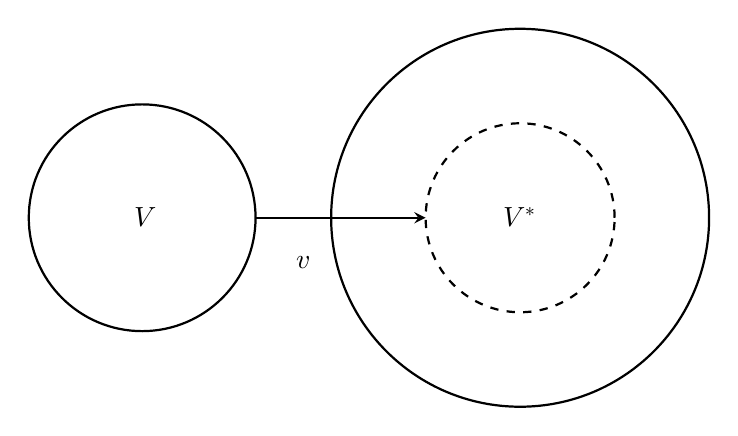
\begin{tikzpicture}[
    >=stealth,
    scale=1.2
]
    % 左侧圆和文字
    \draw[thick] (0,0) circle (1.2) node {$V$};
    
    % 右侧大圆
    \draw[thick] (4,0) circle (2);
    % 右侧虚线圆
    \draw[thick, dashed] (4,0) circle (1) node {$V^*$};
    
    % 箭头与标签
    \draw[thick, ->] (1.2,0) -- (3,0);
    \node[below] at (1.7, -0.3) {$v$};
\end{tikzpicture}
    \caption{线性空间与对偶空间的关系}
    \label{The_relation_between_the_Linear_Space_and_its_CP}
\end{figure}
当然，对于有限维的线性空间，它当然是满足双射的. 但是对于无穷维，就不一定了. 不过，在量子力学的语境下，波函数不能演化着演化着跳出空间了. 所以我们假定波函数所在空间及其对偶都是在Hilbert空间内的，保证完备性(更严谨的数学涉及Riez定理，可以参考相关数目). 我们于是给予内积一个合法的数学来源，接下来可以将Hilbert空间的函数一个基底展开，考虑基函数列\(\{e_{n}\}\)，那么Hilbert空间内的函数\(f\)可以写为：
\[
f = \sum_{n=0}^{\infty}c_{n}e_{n}
\]
考虑正交归一的基底，所以\(c_{n} = \langle e_{n},f\rangle\)，因此：
\[
f = \sum_{n=0}^{+\infty}e_{n}\langle e_{n},f\rangle
\]
而它的对偶空间内的元素为
\[
\langle f,\cdot\rangle = \sum_{n=0}^{+\infty}\langle e_{n},f\rangle\langle e_{n},\cdot\rangle
\]
这种符号不对称，因此我们不妨将表示内积的尖括号拆成两部分：\(\langle f,g\rangle\to\braket{f}{g}\)，\(\bra{f}\)被称为左矢，\(\ket{g}\)被称为右矢. 于是，函数的基底展开写成对称形式：
\begin{align*}
& \ket{f} = \sum_{n=0}^{\infty}\ket{e_{n}}\bra{f_n}\ket{f} \\
& \bra{f} = \sum_{n=0}^{\infty}\bra{f}\ket{e_{n}}\bra{e_{n}}
\end{align*}
这种符号表示，被称为\textbf{Dirac符号}，它体现了原空间与对偶空间的同构关系. 左矢左乘右矢表示内积，那左矢右乘右矢有意义吗？有，这时我们会得到两个矢量对应的\textbf{并矢}，即一个\textbf{(1,1)型张量}. 例如，刚刚分量展开写出的(1,1)型张量对应一个单位矩阵：
\[
\sum_{n=0}^{\infty}\ket{e_{n}}\bra{e_{n}} = 1
\]
这里1不是实数1，而是单位算符1. 明确了量子力学生效的空间与空间内描述运算的语言，我们来正式讨论量子力学中的形式理论. 
\section{态与本征值}
上述一章是为了给Dirac符号一个相对合法的来源，它更多的是数学内容，而不具备那么明显的物理图像. 接下来，我们要用一个右矢来标记一个粒子本身的状态. 那么在介绍具体的数学形式前，我想讲一讲它的物理来源. 回顾经典力学中对于粒子的刻画，我们通常不在意粒子的本体，而在意描述粒子动力学特点的量，最基本的便是位置和动量，即\(\br{\vr,\vp}\). 然而，这种视角的局限性在于，我们没有考虑测量对于系统的影响. 事实上，任何实验在开始时就已经“不准确”了. 举一个非常简单的例子，我们在使用光电门和气垫导轨测量小车下滑速度的时候，如果光电门没有摆好，器材的边缘发生了刮擦，测量这个行为本身就会对已经存在的系统造成影响. 当然，在经典尺度上，这种影响可以规避，但是当我们深入原子亚原子尺度时，已有的光学测量手段总会对测量造成干扰，这时，用决定论的视角再来看问题就不合适了. 原因在于，观测前我们没有看到粒子真实的状态，因此粒子的状态存在多种可能. 这就像投下骰子之前，1-6点数是同时存在的可能结果一样，同理在观测之前粒子的状态是其所有可能结果的叠加，而观测会让粒子的状态\textbf{坍缩}成所有可能中的一种. 一方面，概率论视角下，观测对系统的影响是区分经典与量子最核心的内容；另一方面，这种特点使得粒子的“本体”变成一种可操作对象，同时叠加的特点使得它类似于某种向量. 也因此，我们需要Dirac符号和力学量算符化来重新描述量子力学. 这便是接下来我们要讨论的内容. 
\subsection{态右矢与态左矢}
基于Dirac符号，我们可以将表征粒子状态的类似于矢量的波函数用右矢表示，这时，这种右矢被称为\textbf{态右矢}，记作：
\[
\ket{\al}
\]
其对偶为态左矢，记作：
\[
\bra{\alpha}
\]
其中，左右矢互相对偶. 并且态矢的模可以由其左右矢的内积定义：
\[
|\ket{\al}| = \sqrt{\bra{\al}\ket{\al}}
\]
从矩阵视角来看，左右矢的对偶可以用\textbf{共轭转置}来描述，假设
\[
\ket{\alpha} = (\alpha_{1},\alpha_{2},\cdots)^{T}
\]
那么
\[
\bra{\alpha} = (\al^{*}_{1}, \al^{*}_{2},\cdots)
\]
记共轭转置的符号为上标\(\dagger\)，那么：
\[
\bra{\al} = (\ket{\al})^{\dagger}
\]
明确了描述态的基本语言，我们来看对态的运算. 
\subsection{算符及其本征右矢}
前文我们讨论过对概率波的理解，在这种语境下，力学量的绝对数值没有意义，更有意义的是其数学期望. 对于一个连续的波函数，某一个力学量A的期望为：
\[
\avg{A} = \int A|\Psi|^{2}\dd^{3}{\vr} = \int\Psi^{*}A\Psi\dd^3\vr
\]
我们可以把求期望的积分分成三个部分：共轭波函数+力学量+波函数. 共轭波函数和波函数的关系类似于我们的左态矢和右态矢，似乎可以用Dirac符号抽象，这时力学量则相应抽象为\textbf{算符}. 所以量子力学的情境中，代表绝对数据的力学量\(A\)的适用性是没有代表某种操作的算符\(\uv{A}\)强的. 因此，我们把所有的力学量转化为算符，这时的力学量也换了一个更专业的名字：\textbf{可观测量}. 为了符号的简洁，我们接下来的讨论都省略掉代表算符的\(\uv{}\). 然后，我们开始讨论算符的性质，以及它对于态矢的作用. 
\subsubsection{1. 算符的数学性质}
首先，可观测量的算符对态矢的作用写做：
\[
A(\ket{\al}) = A\ket{\al}
\]
或者，我们写做：
\[
\bra{\be}A^{\dagger} = (A\ket{\be})^{\dagger}
\]
于是很自然的，我们得到结合公理：
\[
(\bra{\be}A^{\dagger})\ket{\al} = \ket{\beta}(A\ket{\al}) = \bra{\be}A\ket{\al}
\]
算符作用于右矢右侧(\(\ket{a}A\))和算符作用于左矢左侧\(A\bra{a}\)是不合法的定义，不存在这样的表述. 然后，可观测量的算符是可加的，满足加法交换律和结合律：
\begin{align*}
& A + B = B + A \\
& A + (B + C) = (A + B) + C
\end{align*}
这种性质反映的实际上是量子力学在测量中的某种不变性. 例如，对于一个庞大的粒子系统，我可以选择抽样，在不影响原本系统状态的条件下抽取一部分粒子，测量其动能\(T\)；然后再抽取另一部分粒子，测量其势能\(U\)；最后抽取一部分粒子，测量其总能量\(E\). 算符的可加性保证了物理结果的匹配，即：
\[
\avg{E} = \avg{T} + \avg{U}
\]
这实际上是Hilbert空间内左右矢线性性的直接体现，也对应着物理现实. 但是，最终结果数值的可加性不代表测量先后的可交换. 例如，我可以把对右矢的算符理解成矩阵，矩阵就是不满足交换律、只满足结合律的：
\begin{align*}
& AB \neq BA \\
& A(BC) = (AB)C
\end{align*}
这意味着，\textbf{固定}测量顺序，中间形式上引入多少个中间“节点”不重要. 
\subsubsection{2. 算符的本征方程}
明确了算符的运算性质和作用规则，我们来看算符的本征方程. 对于一个可观测量，它满足：
\[
A\ket{a} = a\ket{a}
\]
其中\(\ket{a}\)对应本征方程的本征矢，\(a\)对应本征值(也被称为谱). 对可观测量的测量中，我们得到的是其本征值，因此本征值为实数. 对本征方程取共轭转置：
\[
\bra{a}A^{\dagger} = \bra{a}a^{*} = \bra{a}a
\]
因此，两个算符有完全相同的本征值，和对偶的本征矢，不妨把算符想象成矩阵，因此有：
\[
A = A^{\dagger}
\]
这时，算符的性质被称为Hermit，这种算符也被称为Hermit算符. 基于其Hermit性，我们能证明，本征右矢相互正交. 假设算符A对应的本征值构成集合\(\{a_{1},a_{2},\cdots\}\)，那么任意两个本征方程可以写成：
\begin{align*}
& A\ket{a_{i}} = a_{i}\ket{a_{i}} &\cdots && (1) \\
& A\ket{a_{j}} = a_{j}\ket{a_{j}} &\cdots && (2)
\end{align*}
(2)式等价于：
\[
\bra{a_{j}}A = \bra{a_{j}}a_{j} \cdots (2)^{*}
\]
因此\((1)\)式左乘\(\bra{a_{j}}\)，\((2)^{*}\)右乘\(\ket{a_{i}}\)，然后两者相减得到：
\[
(a_{j} - a_{i})\bra{a_{j}}\ket{a_{i}} = 0
\]
当\(a_{i}\neq a_{j}\)时，\(\bra{a_{i}}\ket{a_{j}}=0\)；当\(a_{i}=a_{j}\)时，假定本征矢是归一化了的，那么有\(\bra{a_{i}}\ket{a_{j}}=1\). 我们可以说，这些本征右矢是\textbf{良定义}的，于是很自然的，我们会把态矢量展开成关于本征右矢的形式：
\[
\ket{\al} = \sum c_{a}\ket{a}
\]
利用Fourier技巧，我们可以得到\(c_{a}\)的显式表达式：
\[
c_{a} = \bra{a}\ket{\al}
\]
因此，态矢量可以展开为：
\[
\ket{\al} = \sum \bra{a}\ket{\al}\ket{a} = \sum\ket{a}\bra{a}\ket{\al}
\]
第二个等式对应的表达式会更常用，因为我们可以根据它定义投影算符：
\[
\Lambda_{a} = \sum\ket{a}\bra{a}
\]
其中，投影算符的“模”应该等于1. 这种数学形式启发我们更直观的理解Dirac符号. 实际上它们只是抽象空间的一些元素而已，而这些元素有不同的表现形式. 这些不同的表现形式间通过投影算符相互转化：
\[
\ket{\al} \longleftarrow^{\Lambda_{a}}\longrightarrow\ket{a}
\]
而对于态矢量，我们更直观的理解是：描述一个微观粒子，我们永远无法描述它本身，而是通过描述它的特征来确定一个微观粒子. 这就像我们介绍一个人，只能从这个人表现出的外在特点来描述. 对于微观粒子来说，我们描述其可观测量. 因此，一个抽象的态矢量被一个个可观测的本征矢线性组合起来了. 当这里的\(c_{i}\)变成Kronecker符号时，对粒子的量子力学的描述便退化回经典描述，即从不同可能状态的叠加变成了一个绝对的确定的态. 
\subsubsection{3. 基变换}
对于同一个态，我们可以用不同的本征值表示，这时，有：
\[
\ket{\al} = \sum\ket{a}\bra{a}\ket{\al} = \sum\ket{b}\bra{b}\ket{\al}
\]
而本征矢\(\ket{a}\)和本征矢\(\ket{b}\)之间同样可以利用投影算符相互转化，本征矢相互转化的过程便是\textbf{基变换}. 我们可以将本征矢\(\ket{a}\)是一个N维的列向量，\(\ket{b}\)同样是一个N维的列向量，利用类似构造投影算符的操作，我们有：
\[
\ket{b_{k}} = \sum_{l}\ket{b_{l}}\bra{a_{l}}\ket{a_{k}}
\]
其中，变换算符可以记作：
\[
U = \sum_{l}\ket{b_{l}}\bra{a_{l}}
\]
变换算符实际上可以看作矩阵，而这个算符，满足如下性质：
\begin{align*}
U^{\dagger}U
& = \sum_{m}\sum_{n}\ket{a_{m}}\bra{b_{m}}\ket{b_{n}}\bra{a_{n}} \\
& = \sum_{m}\ket{a_{m}}\delta_{m,n}\bra{a_{n}} \\
& = \sum_{n}\ket{a_{n}}\bra{a_{n}} \\
& = 1
\end{align*}
这种算符，我们称之为\textbf{幺正算符}. 在我们的设定中，幺正算符满足：
\[
\ket{b_{k}} = U\ket{a_{k}}
\]
因此，U的矩阵元可以由如下式子给出：
\[
\bra{a_{l}}U\ket{a_{k}} = \bra{a_{l}}\ket{b_{k}}
\]
这时，如果矩阵\(U\)是已知的话，利用矩阵表示，基变换后新的系数可以写做：
\[
\bra{b_{k}}\ket{\al} = \bra{a_{k}}U^{\dagger}\ket{\al}
\]
所以，基变换的具体表现为，变换后相当于变换算符U的Hermit共轭与变换前的相互作用. 我们接下来看变换对于算符的影响，先看这样一种情况，假设算符不是本征矢\(\ket{a},\ket{b}\)对应的算符\(A,B\)，而是某个另外的算符\(X\)，这时，算符\(X\)可以看作一个矩阵，其矩阵元在本征矢\(\ket{b}\)下写做：
\[
\bra{b_{l}}X\ket{b_{k}}
\]
利用\(\ket{b_{k}} = U\ket{a_{k}}\)得到本征矢\(\ket{a}\)下的矩阵元：
\[
\bra{b_{l}}X\ket{b_{k}} = \bra{a_{l}}U^{\dagger}XU\ket{a_{k}}
\]
在新的本征矢\(\ket{b_{k}}\)下的算符为\(X'\)，那么新态矢和旧态矢的算符满足：
\[
X' = U^{\dagger}XU
\]
新旧算符满足的变换类似于矩阵的相似变换. 这种变换，我们称之为\textbf{幺正变换}. 幺正变换的特点在于，变换前后的算符的迹是不变的，对应于这种算符的本征值之和是不变的. 具体证明如下：
\begin{align*}
\mathrm{tr}(X) 
& = \sum_{k}\bra{a_{k}}X\ket{a_{k}} \\
& = \sum_{k}\sum_{m}\sum_{n}\bra{a_{k}}\ket{b_{m}}\bra{b_{m}}X\ket{b_{n}}\bra{b_{n}}\ket{a_{k}} \\
& = \sum_{m,n}\bra{b_{m}}X\ket{b_{n}}\sum_{k}\bra{b_{n}}\ket{a_{k}}\bra{a_{k}}\ket{b_{m}} \\
& = \sum_{m,n}\bra{b_{n}}\ket{b_{m}}\bra{b_{m}}X\ket{b_{n}} \\
& = \sum_{n}\bra{b_{n}}X\ket{b_{n}}
\end{align*}
再看算符\(A\)和\(B\)的前后变化. 由于\(\ket{b}\)满足本征方程：
\[
B\ket{b_{k}} = b_{k}\ket{b_{k}}
\]
那么B在本征矢变换前的对角元可以通过如下方式导出：
\begin{align*}
& \sum_{n}\bra{a_{m}}B\ket{a_{n}}\bra{a_{n}}\ket{b_{k}} = \sum_{n}b_{k}\bra{a_{m}}\ket{a_{n}}\bra{a_{n}}\ket{b_{k}} \\
\therefore\ 
& \sum_{n}\bra{a_{m}}B\ket{a_{n}}\bra{a_{n}}\ket{b_{k}} = b_{k}\bra{a_{m}}\ket{b_{k}}
\end{align*}
这里的变化逻辑是，我想得到B在本征矢\(\ket{a}\)下的矩阵元，那么我一定需要\(\bra{a_{m}}B\ket{a_{n}}\)，也就是说，我需要把右矢从\(\ket{b}\)转化为\(\ket{a}\)，自然要引入投影\(\sum\ket{a}\bra{a}\). 而从下标来看，我们可以把\(\bra{a}\ket{b}\)看成向量，其余部分从左往右分别看作矩阵元和本征值，即：
\begin{align*}
& \bra{a_{m}}B\ket{a_{n}} = B_{mn} \\
& C_{m} = \bra{a_{m}}\ket{b_{k}}
\end{align*}
对于不同的右矢，它们自然是不正交的，这时要使\(C_{m}\neq 0\)，我们需要满足方程：
\[
\det(B - b_{k}1) = 0
\]
这也就说明\(B\)是可以对角化的. 需要说明的一点在于，B这时要求是Hermit的，否则结论失效. 在明确了B的对角化流程之后，我们比较原本的本征右矢对应的算符A的对角化与B的对角化的关系，将本征矢\(\ket{b}\)变换回本征矢\(\ket{a}\)，于是有：
\[
B\ket{b_{k}} = b_{k}\ket{b_{k}} \Longleftrightarrow BU\ket{a_{k}} = b_{k}U\ket{a_{k}}\Longleftrightarrow U^{\dagger}BU\ket{a_{k}} = b_{k}\ket{a_{k}}
\]
对比态矢\(\ket{a_{k}}\)本身满足的本征方程：
\[
A\ket{a_{k}} = a_{k}\ket{a_{k}}
\]
我们发现，在同在本征矢\(\ket{a}\)下，\(A\)和\(U^{\dagger}BU\)是可以同时对角化的. 那么\(A\)和\(U^{\dagger}BU\)是同一种物理量吗？答案往往是这样的，我们会在后续展示出来. 
\subsection{测量}
承接上文，在对于可以同时对角化的算符，它们有怎样的物理呢？它们物理在于测量的独立性. 所以接下来，我们将从测量的角度继续学习量子力学. 首先，我们给定\textbf{测量公设}. 引用Dirac的原话：测量总是会导致系统跳跃到被测动力学变量的一个本征态. 要理解这个公设，我们从一个直观的例子出发. 假设一个学生只可能出现在教学楼、路上、食堂和路上，这四个位置对应了可观测量位置的四个本征矢，那么这个学生的态可以用这四个本征矢完整表述，即：
\[
student = c_{1}(classroom) + c_{2}(canteen) + c_{3}(road) + c_{4}(dorm)
\]
这时，一个老师观测这个学生，发现他在教室，意味着：
\[
c_{1}(classroom) + c_{2}(canteen) + c_{3}(road) + c_{4}(dorm) \longrightarrow classroom
\]
也就是说学生的状态从多个本征态构成的情形\textbf{坍缩}到了唯一的本征态. 至于说为什么选择的本征态是教室呢？因为老师在教室发现学生的概率是最大的. 也就是说，量子力学的测量实际上包含了一种选择：\textbf{通常}选择概率最大的本征态作为测量结果. 用代数的语言表述出来即是，测量是某种将态矢量坍缩至本征矢的映射：
\[
\ket{\al} -^{\text{测量}}\to \ket{a_{k}}
\]
是否选择这种本征态由其本征矢的系数的模平方决定：
\[
p(\text{测量结果是\(\ket{a_{k}}\)}) = |c_{k}|^{2} = |\bra{a_{k}}\ket{\al}|^{2}
\]
这个时候，我们讨论的虽然是单个粒子的物理系统，但是为了实验确定可观测量A的值，我们必须考虑一个多粒子系统的测量，这时，随着样本足够多，某些小概率事件也会发生，因此测量值会向\textbf{期望值}靠拢. 数学上定义期望的方式为：
\[
\avg{A} = \sum_{k}a_{k}|c_{k}|^{2} = \sum_{k}a_{k}|\bra{a_{k}}\ket{\al}|^{2}
\]
转化为Dirac符号的形式，有：
\begin{align*}
\avg{A}
& = \sum_{k}a_{k}|\bra{a_{k}}\ket{\al}|^{2} \\
& = \sum_{k}a_{k}\bra{\al}\ket{a_{k}}\bra{a_{k}}\ket{\al} \\
& = \sum_{k,l}a_{l}\delta_{l,k}\bra{\al}\ket{a_{l}}\bra{a_{k}}\ket{\al} \\
& = \sum_{k,l}\bra{\al}\ket{a_{l}}\bra{a_{l}}A\ket{a_{k}}\bra{a_{k}}\ket{\al} \\
& = \bra{\al}A\ket{\al}
\end{align*}
在接续讨论多个可观测量测量的问题前，我们要引入\textbf{对易子}：
\[
[A,B] = AB - BA
\]
对易子是检验算符是否满足交换律的工具，为什么要验证交换律呢？因为测量实际上会“毁灭”一个初态，粒子的态矢由于我们的观测收到了干扰，因此要想测量粒子的可观测量，那么先后顺序就是很重要的. 对于某些可观测量，交换测量顺序不会影响结果，而对于另一些则影响，至于影响的具体方式，我们将在接下来的讨论中展开. 
\subsubsection{1. 相容可观测量}
首先，我们直接给出\textbf{相容}的可观测量的概念，即这两个可观测量对易：
\[
[A,B] = 0
\]
相容的可观测量让我们能同时确定这两个量的观测值. 假设\(A,B\)都是在本征矢\(\ket{a_{k}}\)下已知的相容可观测量，那么有：
\begin{align*}
& A\ket{a_{k}} = a_{k}\ket{a_{k}} \\
\therefore\ 
& \bra{a_{l}}[A,B]\ket{a_{k}} = (a_{l} - a_{k})\bra{a_{l}}B\ket{a_{k}} = 0
\end{align*}
这就意味着，当且仅当\(k=l\)时，\(\bra{a_{l}}B\ket{a_{k}}\). 从矩阵视角来看，这实际上代表着，当A可以对角化的时候，如果B与A相容，那么B可以同时对角化. 在继续讨论之前，我们可以辨析一下，基变换中的\(U^{\dagger}BU\)和A的同时对角化与相容物理量\(A,B\)的同时对角化：对于前者，它展现的是可观测量之间的转化关系，例如我们后面会展现的，自旋角动量算符\(S_{x}\)可以通过旋转变换，得到\(S_{z}\)，但是在旋转后测量的就不再是\(S_{x}\)，从实际情景上考虑，旋转变换实际上是将探测器旋转；对于后者，它展现的是可观测量是否可以同时测量的问题. 而对于相容可观测量对应的本征矢和本征值，它们可以构成一个\textbf{共同本征矢}\(\ket{a_{k},b_{k}}\). 这时，算符\(A,B\)可以分别对\(a_{k}\)和\(b_{k}\)作用，即：
\begin{align*}
& A\ket{a_{k},b_{k}} = a_{k}\ket{a_{k},b_{k}} \\
& B\ket{a_{k},b_{k}} = b_{k}\ket{a_{k},b_{k}}
\end{align*}
\subsubsection{2. 不相容可观测量}
接下来我们再看算符不对易的情况，此时两个可观测量的关系被称为\textbf{不相容}的. 对于不相容的物理量，由它们的本征值联合组成的本征右矢\(\ket{a_{k},b_{k}}\)是无意义的. 除开这种特点外，不相容物理量的测量相互影响，无法同时得到测量结果，我们考虑如图\ref{fig:measurement}所示的情景. 
\begin{figure}[htbp]
    \centering
    \begin{subfigure}[b]{0.45\textwidth}
        \centering
        \includegraphics[width=\linewidth]{figures/Measurement1.png}
        \caption{子图 (a) }
        \label{fig:sub-a}
    \end{subfigure}
    \hfill  % 添加水平间距
    \begin{subfigure}[b]{0.45\textwidth}
        \centering
        \includegraphics[width=\linewidth]{figures/Measurement2.png}
        \caption{子图 (b) }
        \label{fig:sub-b}
    \end{subfigure}
    \caption{总图标题：测量过程示意图}
    \label{fig:measurement}
\end{figure}
遮挡表示“不测量”，因此，对于其中一个\(\ket{b'}\)，最终测量到\(\ket{c'}\)的概率为：
\[
|\bra{c'}\ket{b'}|^{2}|\bra{b'}\ket{a'}|^{2}
\]
对\(b'\)求和，得到经过所有的\(b\)的本征矢测量到\(\ket{c'}\)的概率，为：
\[
\sum_{b'}|\bra{c'}\ket{b'}|^{2}|\bra{b'}\ket{a'}|^{2} = \sum_{b'}\bra{c'}\ket{b'}\bra{b'}\ket{a'}\bra{a'}\ket{b'}\bra{b'}\ket{c'}
\]
然而，如果没有中间测量\(B\)的过程，那么最终测量得到\(\ket{c'}\)的概率为：
\[
|\bra{c'}\ket{a'}|^{2} = \Bigg|\sum_{b'}\bra{c'}\ket{b'}\bra{b'}\ket{a'}\Bigg|^{2} = \sum_{b',b''}\bra{c'}\ket{b'}\bra{b'}\ket{a'}\bra{a'}\ket{b''}\bra{b''}\ket{c'}
\]
很明显，是否测量\(B\)可能会对最终结果产生影响. 当且仅当\(B\)与\(A\)或者\(C\)相容的时候，B的测量与否才对最终结果不产生影响. 因此，不相容的物理量，测量的过程中会彼此影响. 
\subsubsection{3. 测不准原理}
这种吧相互影响从测不准原理的角度也能更好的看出来. 定义某一力学量\(A\)的方差为：
\[
\sigma_{A}^{2} = \bra{(\uv{A}-\langle A\rangle)\al}\ket{(\uv{A}-\langle A\rangle)\al}\triangleq \bra{f}\ket{f}
\]
同理，我们也能得到另一个力学量\(B\)的方差：
\[
\sigma_{B}^{2} = \bra{(\uv{B}-\langle B\rangle)\al}\ket{(\uv{B}-\langle B\rangle)\al}\triangleq \bra{g}\ket{g}
\]
这时，利用Cauchy-Schwarz不等式：
\[
\sigma_{A}^2\sigma_{B}^2 \geq \Big(\frac{1}{2i}[\bra{f}\ket{g} - \bra{g}\ket{f}]\Big)^{2}
\]
接下来，我们计算\(\bra{f}\ket{g}\)：
\begin{align*}
\braket{f}{g}
& = \bra{(\uv{A}-\langle A\rangle)\al}\ket{(\uv{B}-\langle B\rangle)\al} \\
& \bra{\al}\ket{(\uv{A}\uv{B} - \langle A\rangle\uv{B} -\uv{A}\langle B\rangle + \langle A\rangle\langle B\rangle)\al} \\
& = \bra{\al}\uv{A}\uv{B}\ket{\al} - \langle A\rangle\bra{\al}\uv{B}\ket{\al} - \langle B\rangle\bra{\al}\uv{A}\ket{\al} + \langle A\rangle\langle B\rangle \bra{\al}\ket{\al} \\
& = \avg{AB} - \avg{A}\avg{B} - \avg{B}\avg{A} + \avg{A}\avg{B} \\
& = \avg{AB} - \avg{A}\avg{B}
\end{align*}
同理，我们可以得到：
\[
\bra{g}\ket{f} = \langle BA\rangle - \avg{A}\avg{B}
\]
注意，\(\uv{A}\)和\(\uv{B}\)的顺序是对期望有影响的，因为计算期望时，力学量算符对态矢量作用，顺序会导致对态矢量的左矢的作用结果不同，进而影响期望结果. 代回不等式，我们得到：
\[
\sigma_{A}^2\sigma_{B}^2 \geq \Big(\frac{1}{2i}[\avg{AB}-\avg{BA}]\Big)^2=\Big(\frac{1}{2i}[A,B]\Big)^{2}
\]
这种不等关系称被称为\textbf{测不准原理}. 为什么测不准？我们以坐标表象下的位置算符和动量算符为例展示，1维位置算符和动量算符为：
\begin{align*}
& {x} = x \\
& {p} = -i\hh\frac{\dd}{\dd x}
\end{align*}
所以二者的对易子(或者叫对易关系)为：
\[
[{x},{p}] = xp - px = -i\hh x\frac{\dd}{\dd x} + i\hh\frac{\dd}{\dd x}x 
\]
动量算符这里相当于求导，所以
\[
px= -i\hh\frac{\dd}{\dd x}x \equiv -i\hh\frac{\dd}{\dd x}(x\cdot) = -i\hh(\cdot) - i\hh x\frac{\dd}{\dd x}(\cdot) = -i\hh - i\hh x\frac{\dd}{\dd x}
\]
代回对易关系，我们得到：
\[
[x,p] = i\hh
\]
因此，坐标和动量的方差满足：
\[
\sigma_{x}^2\sigma_{p}^2 \geq \Big(\frac{\hh}{2}\Big)^2 \Longleftrightarrow \sigma_{x}\sigma_{p} \geq \frac{\hh}{2}
\]
现在我们测量一个粒子的位置，利用探测手段，我们准确捕捉到某一时刻粒子的位置，这时\(\sigma_{x}=0\)，由测不准原理，\(\sigma_{p}\to \infty\). 这就意味着对坐标的单次测量中，动量的不确定度达到无穷大，换言之，我们无法得到动量的信息. 从图像上来理解，我们会发现当粒子位置可以被测准时，它的波函数会对应一个宽度极窄的尖峰，这也就意味着它的谱展开是复杂的，没有办法用单一的波矢来描述，而粒子的动量正比于波矢，因此波矢也无法精确测量；相反，如果粒子有明确的波矢，那么它偏向于一个弥散在空间中的正弦波，这时，粒子的位置是不确定的. 正是这种无法同时测准的性质，我们命名不等式为测不准原理. 而这种测不准的核心来源是不等式右侧不为0，这也就意味着对易关系是否为0可以帮助我们判断两个力学量是否以同时测量. 当力学量算符不对易时，两个测量量的标准差相互影响，无法同时测准这两个力学量. 
\subsection{两种表象}
\subsubsection{1. 连续谱}
对前文讨论的本征方程：
\[
A\ket{a_{k}} = a_{k}\ket{a_{k}}
\]
我们通常假定本征值\(a_{k}\)是离散的，此时，本征值构成的集合称为\textbf{谱}，离散的本征值对应的就是\textbf{离散谱}. 一般来说，其可观测量和本征值分别对应Hamiltonian和能量. 然而，除开能量外，如位置和动量，它们都有连续的本征值. 这种本征值的集合被称为\textbf{连续谱}. 以1维动量算符，我们展示连续谱的特点. 考虑1维的情景，动量算符满足的本征方程为
\[
-i\hh\frac{\dd f_{p}(x)}{\dd x} = pf_{p}(x)
\]
所以求解得到：
\[
f_{p}(x) = A\exp\Big(i\frac{xp}{\hh}\Big)
\]
本征函数平方不可积，因此它实际上不在我们限定的Hilbert空间内. 然而，限定动量取值为实数，我们依旧可以计算动量算符对应本征函数的正交性：
\begin{align*}
\int_{\infty}f^{*}_{p'}(x)f_{p}(x)\dd x 
& = |A|^2\int_{\infty}\exp\Big[i\frac{x}{\hh}(p-p')\Big]\dd x \\
& = 2\pi\hh|A|^{2}\delta(p-p')
\end{align*}
令系数归一，有\(A = 1/\sqrt{2\pi\hh}\)，所以，动量算符的本征函数为：
\[
f_{p}(x) = \frac{1}{\sqrt{2\pi\hh}}\exp\Big(i\frac{xp}{\hh}\Big)
\]
因此，简单来说，我们只需要把离散谱的所有表达连续化即可，假设具有连续本征值的可观测量为\(\xi\)，那么：
\begin{align*}
& \bra{\xi''}\ket{\xi'} = \delta(\xi''-\xi') \\
& \int\dd\xi'\ket{\xi'}\bra{\xi'} = 1 \\
& \int\dd\xi'|\bra{\xi'}\ket{\al}|^{2} = 1 \\
& \bra{\be}\ket{\al} = \int\dd\xi' \bra{\be}\ket{\xi'}\bra{\xi'}\ket{\al}
\end{align*}
\subsubsection{2. 坐标表象与动量表象}
明确了连续谱的性质，我们来介绍\textbf{表象}. 在前文的推导中，就已经出现了动量算符的表达式：
\[
p = -i\hh\partial_{x}
\]
然而，这种表达式是唯一的吗？并非，实际上这个表达式只是在\textbf{坐标表象}下才成立. 那我们又要问，什么是坐标表象？简单理解，坐标表象即\textbf{以坐标为自变量}. Dirac符号让我们将一个粒子的态看成是Hilbert空间的一个抽象矢量，而不同的表象则赋予了它不同的函数形式. 以经典系统为例，对于一个粒子的位矢，它就是一个抽象的矢量\(\vr\)，要具体计算矢量的模或者其他什么量的时候，我们需要在具体的坐标系中展开位矢. 也就是说，同一个位矢可能有如下三种不同的表达式：
\[
\vr = x\uv{x} + y\uv{y} + z\uv{z} = \rho\uv{\rho} + z\uv{z} = r\uv{n}
\]
它们三个分别对应Cartesian坐标、柱坐标和球坐标. 不规范的说，我们可以分别成为“Cartesian表象”、“柱表象”和“球表象”. 而在量子力学中，我们仅讨论两种表象：以坐标为自变量的\textbf{坐标表象}和以动量为自变量的\textbf{动量表象}. 首先看坐标表象，这时，一个态矢可以利用投影展开成关于自变量的形式：
\[
\ket{\al} = \int\dd x\ket{x}\bra{x}\ket{\al}
\]
其中，\(\bra{x}\ket{\al}\)正是坐标表象下的\textbf{波函数}. 这时，一个粒子处在某一位置\(x'\)的概率为：
\[
\dd{p} = |\bra{x}\ket{\al}|^{2}_{x=x'}\dd{x}
\]
同时，波函数本身可以归一化为：
\[
\bra{\al}\ket{\al} = \int\dd{x}\bra{\al}\ket{x}\bra{x}\ket{\al} = \int\dd{x}|\bra{x}\ket{\al}|^{2}
\]
所有的理论可以推广到3维，于是有：
\[
\ket{\al} = \int\dd^3\vr \ket{\vr}\bra{\vr}\ket{\al}
\]
这时，一个3维的坐标左矢可以写成：
\[
\ket{\vr} = \ket{x,y,z}
\]
是一个由\(\ket{x},\ket{y},\ket{z}\)构成的本征右矢，并且分量之间满足：
\[
[x_{i},x_{j}] = 0, \ \ i,j = 1,2,3
\]
对于坐标表象的讨论，我们还需要考虑\textbf{平移}的问题. 定义平移算符为\(\mathscr{J}\)：
\[
\trans(x') \Longleftrightarrow \text{向右平移}x'\text{个单位}
\]
为了讨论基本性质，我们对这种变换做“微分”，也就是取\textbf{无穷小变换}，得到：
\[
\trans(\dd{\vr})
\]
此时，当无穷小算符作用于坐标本征右矢时，有：
\[
\trans(\dd{\vr})\ket{\vr} = \ket{\vr + \dd{\vr}}
\]
当无穷小算符作用于态右矢时，有：
\[
\trans(\dd{\vr})\ket{\al} = \trans(\dd\vr)\int\dd^3\vr\ket{\vr}\bra{\vr}\ket{\al} = \int\dd^3\vr\ket{\vr+\dd\vr}\bra{\vr}\ket{\al} = \int\dd^3\vr\ket{\vr}\bra{\vr-\dd\vr}\ket{\al}
\]
因此，对于算符的平移实际上是对波函数\(\bra{\vr}\ket{\al}\)下的反向平移，这体现了变换的主动和被动视角. 明确了平移算符与态右矢、本征右矢的作用后，我们考虑算符本身的性质，简单来说，我们考虑算符的逆与算符的叠加. 从集合直观理解，平移算符是可乘的，即：
\[
\trans(\dd\vr_{1} + \dd\vr_{2}) = \trans(\dd\vr_{1})\trans(\dd\vr_{2})
\]
并且，向右平移\(\dd\vr\)的逆是向左平移相同的长度，于是：
\[
\trans(-\dd\vr) = \trans^{-1}(\dd\vr)
\]
同时，由于平移后的态矢\(\trans(\dd\vr)\ket{\al}\)依然是可以归一化的，于是有：
\[
\bra{\al}\ket{\al} = \bra{\al}\trans^{\dagger}(\dd\vr)\trans(\dd\vr)\ket{\al} = 1
\]
因此，平移算符是幺正的：
\[
\trans^{\dagger}(\dd\vr)\trans(\dd\vr) = 1
\]
接着，明确了算符的基本性质，我们考虑算符的\textbf{微扰展开}. 由于
\[
\lim_{\dd\vr\to 0}\trans(\dd\vr) = 1
\]
因此：
\[
\trans(\dd\vr) = 1 - i\mathbf{K}\cdot\dd{\vr}
\]
其中\(\mathbf{K}\)的分量都是Hermit算符. 将它带入上述的对于平移算符的可乘性和幺正性，可以证明基本性质. 在这些基础上，我们讨论平移算符和位矢\(\vr\)的对易关系，首先我们计算则两个式子：
\begin{align*}
& \vr\trans(\dd\vr')\ket{\vr'} = \vr\ket{\vr'+\dd\vr'} = (\vr'+\dd\vr')\ket{\vr'+\dd\vr'} \\
& \trans(\dd\vr')\vr\ket{\vr'} = \vr'\trans(\dd\vr')\ket{\vr'} = \vr'\ket{\dd\vr'+\dd\vr'}
\end{align*}
于是有：
\[
[\vr,\trans(\dd\vr')]\ket{\vr'} = \dd\vr'\ket{\vr'+\dd\vr'} \simeq \dd\vr'\ket{\vr'} \Longleftrightarrow [\vr,\trans(\dd\vr')] = \dd\vr'
\]
然后，带入微扰展开，有：
\[
[\vr,1-i\mathbf{K}\cdot\dd\vr'] = -i[\vr,\mathbf{K}\cdot\dd\vr'] = -i\sum_{i}[x_{i},K_{j}]\dd{x}_{j}\uv{x}_{i} = \dd\vr' 
\]
最终化简我们得到：
\[
[x_{i},K_{j}] = i\delta_{ij}
\]
上述的讨论自然是非常数学的，明确了数学的基本性质之后，我们需要理解，平移算符的微扰展开的系数\(\mathbf{K}\)究竟对应着什么物理呢？这个时候我们需要从经典力学出发反过来得到量子力学的对应. 参考Goldstein的《经典力学》，平移变换的生成函数由动量给出：
\[
F(\vr,\mathbf{P}) = \vr\cdot\mathbf{P} + \vp\cdot\dd\vr
\]
这个式子和平移算符的微扰展开形式上类似，结合\(\mathbf{K}\)量纲是\(\mathrm{m}^{-1}\)，于是不妨定义：
\[
\mathbf{K} = \frac{\mathbf{p}}{\hh}
\]
这时，得到：
\begin{align*}
& \trans(\dd\vr) = 1 - i\frac{\vp\cdot\dd\vr}{\hh} \\
& [x_{i},p_{j}] = i\hh\delta_{ij}
\end{align*}
这样我们便从算符的角度直接得出了位置与动量的对易关系，而不依赖于坐标表象中位置算符和动量算符的表达式. 对于量子的对易关系，我们可以类比经典的对易关系或者说是Poisson括号：
\[
[x_{i},p_{j}] = \delta_{ij}
\]
因此，经典与量子之间的对应为：
\[
[,]_{\text{经典}} \longleftrightarrow \frac{[,]_{\text{量子}}}{i\hh}
\]
得到了\(\mathbf{K}\)的具体物理含义，我们可以根据其性质得到\(\vp\)的性质. 在讨论这个问题之前，我们首先需要明确无穷小平移和有限长度平移的关系. 假设平移的长度是有限长\(\Delta{x}\)，我们可以将其看作无限个无穷小平移的“叠加”，也就是：
\[
\trans(\Delta{x}\uv{x}) = \lim_{N\to\infty}\Big(1 - i\frac{p_{x}\Delta{x}}{\hh}\Big)^{N} = \exp(-\frac{ip_{x}\Delta{x}}{\hh})
\]
明确了有限平移的表达式，我们可以利用其可乘性：
\begin{align*}
& \trans(\Delta{x}\uv{x})\trans(\Delta{y}\uv{y}) = \trans(\Delta{y}\uv{y})\trans(\Delta{x}\uv{x}) = \trans(\Delta{x}\uv{x} + \Delta{y}\uv{y})
\end{align*}
于是有：
\[
[\trans(\Delta{x}\uv{x}),\Delta{y}\uv{y}] = 0
\]
这时，将平移算符Taylor展开到2阶，我们能将平移算符的对易关系转化为对动量算符的对易关系：
\begin{align*}
[\trans(\Delta{x}\uv{x}),\Delta{y}\uv{y}] 
& = \Bigg[\Big(1-\frac{ip_{x}\Delta{x}}{\hh}-\frac{p_{x}^{2}(\Delta{x})^{2}}{2\hh^2}\Big) , \Big(1-\frac{ip_{y}\Delta{y}}{\hh}-\frac{p_{y}^{2}(\Delta{y})^{2}}{2\hh^2}\Big)\Bigg] \\
& = \Big(1 - i\frac{p_{x}\Delta{x}+p_{y}\Delta{y}}{\hh} - \frac{p_{x}^{2}(\Delta{x})^{2} + p_{y}^{2}(\Delta{y})^{2}}{2\hh^2}\Big) - \frac{\Delta{x}\Delta{y}(p_{x}p_{y}-p_{y}p_{x})}{\hh^2} \\
& - \Big(1 - i\frac{p_{x}\Delta{x}+p_{y}\Delta{y}}{\hh} - \frac{p_{x}^{2}(\Delta{x})^{2} + p_{y}^{2}(\Delta{y})^{2}}{2\hh^2}\Big) \\
& = -\frac{\Delta{x}\Delta{y}[p_{x},p_{y}]}{\hh^2} = 0 \\
\Longrightarrow 
& [p_{x},p_{y}] = 0
\end{align*}
推广至3维，我们得到动量算符中的对易关系：
\[
[p_{i},p_{j}] = 0
\]
而这种生成元对易所对应的群称为\textbf{Abel群}. 最后需要讨论的是平衡算符对于动量算符的作用：
\[
\trans(\dd{\vr}')\ket{\vp'} = \Big(1 - i\frac{\vp\cdot\dd\vr'}{\hh}\Big)\ket{\vp'} = \Big(1 - i\frac{\vp'\cdot\vr'}{\hh}\Big)\ket{\vp'}
\]
这就意味着动量本征右矢实际上是平移算符的本征右矢，然而由于其本征值是复数，所以平移算符为非Hermit的. 讨论完坐标和动量本征右矢的性质后，我们终于可以讨论这两种表象下算符的具体形式. 在坐标表象下，由Hamiltonian得到它们的具体形式为：
\begin{align*}
& \vr = \vr \\
& \vp = -i\hh\nabla
\end{align*}
或者我们可以得到1维的形式：
\begin{align*}
& x = x \\
& p = -i\hh\dd{}{x}
\end{align*}
考虑动量算符在态右矢上的作用，得到：
\[
p\ket{p'} = p'\ket{p'}
\]
两边作用\(\bra{x}\)，我们得到坐标表象下的态右矢对应的本征函数：
\[
-i\hh\de{}{x}\bra{x}\ket{p'} = p'\bra{x}\ket{p'} \Longrightarrow \bra{x}\ket{p'} = A\exp\Big(i\frac{xp'}{\hh}\Big)
\]
归一化，可以得到\(A=\frac{1}{\sqrt{2\pi\hh}}\)，因此，坐标表象下动量算符的本征函数为：
\[
\bra{x}\ket{p'} = \frac{1}{\sqrt{2\pi\hh}}\exp\Big(i\frac{xp'}{\hh}\Big)
\]
推广到3维，本征函数推广成：
\[
\bra{\vr}\ket{\vp} = \frac{1}{(2\pi\hh)^{\frac{3}{2}}}\exp\Big(i\frac{\vr\cdot\vp}{\hh}\Big)
\]
而在动量表象下，我们可以进行如下变换(考虑1维情形)：
\begin{align*}
\bra{p}x\ket{\al}
& = \int\bra{p}x\ket{p'}\bra{p'}\ket{\al}\dd p' \\
& = \int\dd p' \int\dd x'\int\dd x'' \bra{p}\ket{x'}\bra{x'}\uv{x}\ket{x''}\bra{x''}\ket{p'}\bra{p'}\ket{\al} \\
& = \int\dd p' \int\dd x'\int\dd x''{\bra{x'}\ket{p}}^{*}x'\delta(x'-x'')\bra{x''}\ket{p'}\bra{p'}\ket{\al} \\
& = \int\dd p' \int\dd x'x'{\bra{x'}\ket{p}}^{*}\bra{x'}\ket{p'}\bra{p'}\ket{\al} \\
& = \frac{1}{2\pi\hh}\int\dd p'\int\dd x'x'\exp\Big(i\frac{x'p'-p x'} {\hh}\Big)\bra{p'}\ket{\al} \\
& = \frac{1}{2\pi\hh}\int\dd p'\int\dd x' i\hh\pd{}{p}\exp\Big(i\frac{p-p'}{\hh}x'\Big)\bra{p'}\ket{\al} \\
& = i\hh\pd{}{p}\int\dd p'\delta(p-p')\braket{p'}{\al} \\
& = i\hh\pd{}{p}\braket{p}{\al} \\
& = \bra{p}i\hh\pd{}{p}\ket{\al}
\end{align*}
\subsubsection{3. 波函数}
接下来我们看波函数. 波函数实际上是态矢量在某种表象下的具体表现，更通俗的说，态矢量像函数的符号\(f(\cdot)\)，而表象给这个函数填入了合适的自变量. 例如坐标表象下，函数就变成\(f(\vr)\). 
在将态矢量变成波函数的操作中，我们通过两个矢量生成了一个数，这种运算实际上可以用\textbf{内积}描述，因此，特定表象下的波函数可以定义为：
\[
\psi(a) = \bra{a}\ket{\al}
\]
其中，\(\ket{a}\)是某个表象下的本征右矢，\(\ket{\al}\)是态矢量. 我们讨论两个常用的：坐标表象和动量表象. 前面我们讨论过，不同本征右矢间可以变换，那么不同表象间也能变换，利用投影算符，
我们能得到两种表象波函数下的变换关系：
\begin{align*}
\bra{\vr}\ket{\al} = \psi(\vr)
& = \int\dd\vp\bra{\vr}\ket{\vp}\bra{\vp}\ket{\al} \\
& = \frac{1}{(2\pi\hh)^{\frac{3}{2}}}\int\dd\vp\exp\Big(i\frac{\vr\cdot\vp}{\hh}\Big)\bra{\vp}\ket{\al} \\
& = \frac{1}{(2\pi\hh)^{\frac{3}{2}}}\int\dd\vp \phi(\vp)\exp\Big(i\frac{\vr\cdot\vp}{\hh}\Big)
\end{align*}
同理可以得到从动量表象转换成坐标表象：
\[
\phi(\vp) = \frac{1}{(2\pi\hh)^{\frac{3}{2}}}\int\dd\vr \psi(\vr)\exp\Big(-i\frac{\vr\cdot\vp}{\hh}\Big)
\]
因此，两种表象下的波函数变换满足Fourier变换. 
\section{态的时间演化}
我们在这之上讨论了很多相对数学的东西，整理回顾一下，我们可以抓住这样一个思路. Hilbert空间和Dirac符号为抽象描述粒子的状态提供了有效的数学语言：态右矢和算符. 而为了更好的体现
可观测量在微观领域体现的波动性，我们引入算符来表示可观测量，并详细讨论了算符的数学性质、算符与态矢的作用以及在观测中，算符表现的性质. 明确了抽象的态，我们随之讨论了态的表象，并得到了生成
这些表象的本征矢它们的数学性质. 然而，上述的讨论都没有考虑时间的演化. 于是，接下来，我们把这一点补充上. 
\subsection{时间演化算符}
为了表述右态矢的时间演化，我们将时间\(t\)引入，得到：
\[
\ket{\al,t_{0};t}
\]
其中，\(t_{0}\)是初始时刻，\(t\)是当前时刻. 当\(t\to t_{0}\)时，\(\ket{\al,t_{0};t}\to\ket{\al}\). 除开极限关系，我们需要知道从\(\ket{\al}\)到\(\ket{\al},t;t_{0}\)的演化规律，
于是，我们引入\textbf{时间演化算符}，记为\(\cU(t,t_{0})\). 因此有：
\[
\ket{\al,t_{0};t} = \cU(t,t_{0})\ket{\al,t_{0}}
\]
接下来，我们讨论时间演化算符的性质，基于之前的经验，我们的讨论从幺正性、叠加规则、微扰展开等方面展开. 首先看幺正性，由于演化前后，右态矢都应该是可以被归一化的，于是：
\[
\bra{\al,t_{0};t}\ket{\al,t_{0};t} = \bra{\al,t_{0}}\cU^{\dagger}(t_{0},t)\cU(t_{0},t)\ket{\al,t_{0}} = 1
\]
因此：
\[
\cU^{\dagger}(t_{0},t)\cU(t_{0},t) = 1
\]
幺正性具有必然性，由于概率流守恒，一旦右态矢被归一化，它将一直保持归一化. 接下来，我们讨论时间算符的叠加. 由于时间具有连续性，所以从\(t_{0}\)到\(t_{1}\)再到\(t_{2}\)和从\(t_{0}\)
直接到\(t_{2}\)的演化应保持结果一致，因此：
\[
\cU(t_{0},t_{2}) = \cU(t_{0},t_{1})\cU(t_{1},t_{2})
\]
明确了算符的基本性质，我们开始对非线性的算符做微扰展开：
\[
\cU(t_{0}+\dd t,t_{0}) = 1 - i\Omega\dd{t}
\]
利用微扰展开可以证明时间演化算符的叠加性质和幺正性，同时，我们还能得到微扰系数的Hermit性：
\[
(1+i\Omega^{\dagger}\dd{t})(1- i\Omega\dd{t}) = 1 + i\Omega^{\dagger}\dd{t} - i\Omega\dd{t} = 1 \Longrightarrow \Omega^{\dagger} = \Omega
\]
在量纲上，由于\(\Omega\)乘以时间\(t\)是无量纲的，所以\(\Omega\)的量纲为频率，为了保证和在经典化后可以与已有理论匹配，我们定义：
\[
\Omega = \frac{H}{\hh}
\]
其中，\(H\)位Hamiltonian，因此：
\[
\cU(t_{0}+\dd{t},t_{0}) = 1 - i\frac{H}{\hh}\dd{t}
\]
这时，我们可以从另外一个视角推导Schrodinger方程，考虑演化模态减去演化初态：
\[
\cU(t+\dd{t},t_{0}) - \cU(t,t_{0}) = -i\frac{H}{\hh}\dd{t}
\]
将微元\(\dd{t}\)除过去得到：
\[
i\hh\partial_{t}\cU(t,t_{0}) = H\cU(t,t_{0})
\]
这时作用于右矢，得到：
\[
i\hh\partial_{t}\cU(t,t_{0})\ket{\al,t_{0}} = H\cU(t,t_{0})\ket{\al,t_{0}} 
\]
也就是：
\[
i\hh\partial_{t}\ket{\al,t_{0};t} = H\ket{\al,t_{0};t}
\]
接下来，我们讨论有限时间长度\(t-t_{0}\)的时间算符\(\cU\). 然而这个时候需要分三种情况讨论：
\subsubsection{1. Hamiltonian不含时}
这时，我们可以直接将所有无限小时间演化直接叠加，得到：
\[
\lim_{N\to\infty}\Big[1 - i\frac{H}{\hh}\frac{(t-t_{0})}{N}\Big]^{N} = \exp\Big[-i\frac{H}{\hh}(t-t_{0})\Big]
\]
\subsubsection{2. Hamiltonian含时}
若Hamiltonian含时，我们需要分为含时对易和含时不对易两种情况：
\paragraph{(1) 含时对易}
这时，时间演化算符等效为：
\[
\cU(t,t_{0}) = \exp\Big[-\frac{i}{\hh}\int_{t_{0}}^{t}\dd{t'}H(t')\Big]
\]
\paragraph{(2)含时不对易}
这里我们只给出形式解，其具体意义在微扰背景下的相互作用绘景有明确意义
\[
\cU(t,t_{0}) = 1 + \sum_{n=1}^{\infty}\int_{t_{0}}^{t}\dd{t}_{1}\int_{t_{0}}^{t_{1}}\dd{t}_{2}\cdots\int_{t_{0}}^{t_{n-1}}\dd{t}_{n}H(t_{1})H(t_{2})\cdots H(t_{n})
\]

明确了时间演化算符的具体形式，我们讨论算符对应的本征右矢. 假设Hamiltonian不含时，考虑本征方程：
\[
H\ket{a} = E_{a}\ket{a}
\]
利用本征右矢\(\ket{a}\)展开设定\(t_{0}=0\)时间演化算符，得到：
\begin{align*}
\exp(-\frac{H}{\hh}t) 
& = \sum_{i,j}\ket{a_{i}}\bra{a_{i}}\exp(-i\frac{H}{\hh}t)\ket{a_{j}}\bra{a_{j}} \\
& = \sum_{i,j}\ket{a_{i}}\exp(i\frac{E_{i}}{\hh}t)\bra{a_{i}}
\end{align*}
因此，含时演化的态矢可以展开写成：
\begin{align*}
\ket{\al,0;t} 
& = \cU(t,0)\ket{\al} \\
& = \exp(i\frac{H}{\hh}t)\sum_{i}\ket{a_{i}}\bra{a_{i}}\ket{\al,0} \\
& = \sum_{i,j}\ket{a_{j}}\exp(-i\frac{E_{j}}{\hh}t)\bra{a_{j}}\ket{a_{i}}\bra{a_{i}}\ket{\al,0} \\
& = \sum_{i}\ket{a_{i}}\exp(-i\frac{E_{i}}{\hh}t)\bra{a_{i}}\ket{\al,0} \\
& = \sum_{i}\ket{a_{i}}\bra{a_{i}}\ket{\al,0}\exp(-i\frac{E_{i}}{\hh}t)
\end{align*}
这时，我们便得到了某一个态右矢随时间的演化规律. 假设一个可观测量\(A\)的态矢量正好对应单一的本征右矢，那么其期望值满足如下特点：
\[
\avg{A} = \bra{a}\exp(i\frac{E_{a}}{\hh}t)A\exp(-i\frac{E_{a}}{\hh}t)\ket{a} = \bra{a}A\ket{a}
\]
这时，可观测量在能量本征右矢的期望值不含时，因此被证伪能量本征态的\textbf{稳定态}. 注意，即使\(A\)与\(H\)不相容，也不意味着\(A\)不可以和\(H\)有共同本征态，
只是我们要求这个态一定是\([A,H]\)的零本征态. 而在后续的讨论中，我们通过区分可观测量和哈密顿量是否相容来判断可观测量是否守恒，然而，即使一个可观测量存在定态，也不能说它是守恒的，
因为定态的产生依赖于初始条件. 假设某个可观测量对应的态矢是一组本征右矢之和
\[
\ket{\al} = \sum_{i}\ket{a_{i}}\bra{a_{i}}\ket{\al}\exp(-i\frac{E_{i}}{\hh}t) \triangleq \sum_{i}c_{i}\ket{a_{i}}\exp(-i\frac{E_{i}}{\hh}t)
\]
那么这时，其期望值为：
\begin{align*}
\avg{A}
& = \sum_{i,j}c_{j}^{*}\bra{a_{j}}\exp(i\frac{E_{j}}{\hh}t)\cdot{A}\cdot c_{i}\exp(-i\frac{E_{j}}{\hh}t)\ket{a_{i}} \\
& = \sum_{i,j}c_{j}^{*}c_{i}\bra{a_{j}}A\ket{a_{i}}\exp(i\frac{E_{j} - E_{i}}{\hh}t)
\end{align*}
期望值会出现振荡，振荡的频率为：
\[
\omega_{ij} = \frac{E_{j} - E_{i}}{\hh}
\]
这个频被称为\textbf{Bohr频率}. 
\subsection{Schrodinger绘景与Heisenberg绘景}
对于时间演化的理解有两种，这两种理解我们统一从幺正算符开始讨论. 时间演化依旧可以理解成态矢的变换，即：
\[
\ket{\al} \longrightarrow U\ket{\al}
\]
其中算符U被称为幺正算符. 假设存在一个可观测量对应的算符\(X\)作用于态矢，那么前后不同态矢的内积的变化为：
\[
\bra{\be}X\ket{\al} \Longrightarrow \bra{\be}U^{\dagger}XU\ket{\al}
\]
对于这种改变，我们有两种理解：
\begin{itemize}
\item 方法1：\(\ket{\al}\to U\ket{\al}\)，但是算符不改变
\item 方法2：\(X\to U^{\dagger}XU\)，但是右态矢不变
\end{itemize}
两种不同的理解方式可以得到两种描述量子力学的\textbf{绘景}，前者被称为Schrodinger绘景，后者被称为Heisenberg绘景. 从Schrodinger绘景出发理解含时演化规律
我们能导出Schrodinger方程：
\[
i\hh\partial_{t}\ket{\al,t} = H\ket{\al,t}
\]
而从Heisenberg视角出发理解，我们有：
\begin{align*}
\dt{A_{H}}
& = \pdt{\cU^{\dagger}}A_{S}\cU + \cU^{\dagger}A_{S}\pdt{\cU} + \cU^{\dagger}\pdt{A_{S}}\cU \\
& = -\frac{1}{i\hh}\cU^{\dagger}HA_{S}\cU + \frac{1}{i\hh}\cU^{\dagger}A_{S}H\cU + \cU^{\dagger}\pdt{A_{S}}\cU \\
& = -\frac{1}{i\hh}\cU^{\dagger}H\cU\cU^{\dagger}A_{S}\cU + \frac{1}{i\hh}\cU^{\dagger}A_{S}\cU\cU^{\dagger}H\cU + \cU^{\dagger}\pdt{A_{S}}\cU \\
& = \frac{1}{i\hh}[A_{H},\cU^{\dagger}H\cU] + \pdt{A_{H}}
\end{align*}
很明显，\([\cU,H] = 0\)，于是有：
\[
\cU^{\dagger}H\cU = H
\]
于是，我们得到了在Heisenberg绘景下，力学量随时间的演化规律：
\[
\dt{A_{H}} = \pdt{A_{H}} + \frac{1}{i\hh}[A_{H},H]
\]
当力学量不显含时间时，我们有：
\[
\dt{A_{H}} = \frac{1}{i\hh}[A_{H},H]
\]
这个对易关系与时间全导数的关系被称为\textbf{Heisenberg运动方程}. 基于方程，我们得到结论，判断力学量是否守恒，实际上是判断其是否与Hamiltonian对易. 参考经典力学的表达式，我们发现对于只包含广义坐标\(q\)和正则动量\(p\)的可观测量，有：
\[
\dt{A} = [A,H]
\]
所以，我们法线将经典系统量子化只需要做如下操作：
\[
[,]_{\text{经典}} \longleftrightarrow \frac{[,]_{\text{量子}}}{i\hh}
\]
然而，量子力学中的可观测量不一定有经典对应，例如自旋. 这时，更合理的说法实际上是量子力学经典化的方法是：
\[
\frac{[,]_{\text{量子}}}{i\hh}\longleftrightarrow [,]_{\text{经典}}
\]
这种规则被称为\textbf{Dirac正则量子化规则}. Heisenberg运动方程的作用是架起经典和量子的桥梁，下面我们简单看一下应用. 两边对可观测量取均值，有：
\[
\dt{\avg{A}} = \frac{1}{i\hh}\avg{[A,H]} = \frac{i}{\hh}\avg{[H,A]}
\]
这时，带入\(A = x\)和\(A = p\)，有：
\begin{align*}
\dt{\avg{x}}
& = \frac{i}{\hh}\avg{[H,x]} \\
& = \frac{i}{\hh}\avg{Hx - xH} \\
& = \frac{i}{\hh}\avg{\frac{p^2}{2m}x + Ux - x\frac{p^2}{2m} - xU} \\
& = \frac{i}{2m\hh}\avg{[p^2,x]} \\
& = \frac{i}{2m\hh}\avg{p[p,x] - p[x,p]} \\
& = \frac{i}{2m\hh}\avg{p(-i\hh) - i\hh p} \\
& = \frac{\avg{p}}{m}
\end{align*}
\begin{align*}
\dt{\avg{p}} 
& = \frac{i}{\hh}\avg{[H,p]} \\
& = \frac{i}{\hh}\avg{Hp - pH} \\
& = \frac{i}{\hh}\avg{\frac{[p^2,p]}{2m} + [U,p]} \\
& = \frac{i}{\hh}\avg{Up - pU}\\
& =^{\text{坐标表象}}= \frac{i}{\hh}\avg{-i\hh U\frac{\dd}{\dd x} + i\hh\frac{\dd}{\dd x}\cdot U} \\
& = \frac{i}{\hh}\avg{-i\hh U\frac{\dd}{\dd x} + i\hh U\frac{\dd}{\dd x} + i\hh\frac{\dd U}{\dd x}}
 = -\Big\langle{\frac{\dd U}{\dd x}}\Big\rangle
\end{align*}
这让我们得到两个等式：
\begin{align*}
& \dt{\avg{{x}}} = \frac{\avg{{p}}}{m}  \\
& \dt{\avg{{p}}} = -\Big\langle\frac{\dd U}{\dd x}\Big\rangle
\end{align*}
推广至3维，有：
\begin{align*}
& \dt{\avg{\vr}} = \frac{\avg{\vp}}{m} \\
& \dt{\avg{\vp}} = -\avg{\nabla U}
\end{align*}
发现式子与经典力学的Newton第二定律形式完全一致. 这一对等式被证伪\textbf{Ehrenfest定理}，它反映了微观粒子位置和动量的均值按照经典的规律演化. 从物质波的
视角来看，这个定理说的实际上是粒子的波包中心演化符合经典规律. 明确了Heisenberg绘景下算符的特点，我们讨论算符对应的本征右矢的演化规律. 考虑\(t=0\)时刻，
和\(t\)时刻的本征方程：
\begin{align*}
& A_{H}\ket{a,t}_{H} = a\ket{a,t}_{H} \\
& A_{H,0}\ket{a} = a\ket{a}
\end{align*}
根据Heisenberg绘景中对于算符含时演化的理解，有：
\[
A_{H} = \cU^{\dagger}A_{H,0}\cU
\]
于是，将初始时刻的本征方程转变为\(t\)时刻的本征方程，有：
\[
\cU^{\dagger}A\cU\cU^{\dagger}\ket{a} = a\cU^{\dagger}\ket{a}
\Longrightarrow A_{H}\Big(\cU^{\dagger}\ket{a}\Big) = a\Big(\cU^{\dagger}\ket{a}\Big)
\]
这时，对比会发现，本征右矢随事件的演化为：
\[
\ket{a,t}_{H} = \cU^{\dagger}\ket{a}
\]
\textbf{总结：}本节我们的讨论比较数学，但是物理图像是清晰的. 由于量子力学对粒子的描述从确定的位置和动量变成了“不确定”的概率，更合适的刻画的方法便是使用
抽象的态矢量和本征矢. 这不仅会让我们清晰的看到测量是坍缩到本征值或本征函数，还能更简洁的表现粒子演化的规律，并将测量与理论结合起来. 
\section{角动量的形式理论}
对于角动量的讨论通常与\textbf{转动}关联，而在经典力学中，讨论质点的转动通常固定了特定轨道，这时，描述轨道我们更喜欢使用与距离和夹角直接相关的坐标系. 
在2维中，这种坐标系对应极坐标系；在3维中，这种坐标系对应球坐标系. 所以接下来，我们将讨论球坐标系下，能量本征方程的解，进而讨论有关角动量的性质. 
坐标表象下，有：
\[
H\bra{\vr}\ket{a} = \br{-\frac{\hh^2}{2m}\nabla^2 + U(\vr)}\bra{\vr}\ket{a} = E\bra{\vr}\ket{a}
\]
这里，我们考虑与角度无关的中心势，同时在球坐标系下做分解，于是有：
\[
-\frac{\hh^2}{2m}\Bigg[\frac{1}{r^2}\pd{}{r}\Big(r^2\pd{}{r}\Big) + \frac{1}{r^2\sin\theta}\pd{}{\theta}\Big(\sin\theta\pd{}{\theta}\Big) + \frac{1}{r^2\sin^2\theta}\pdd{}{\phi}\Bigg]\bra{\vr}\ket{a} = (E-U)\bra{\vr}\ket{a}
\]
将本征函数做分离变量，有\(\bra{\vr}\ket{a} = R(r)Y(\theta,\phi)\)，带入，可以得到两个本征方程：
假定势能仅与到原点距离相关，我们可以将方程分成2个部分：
\[
\underbrace{\frac{1}{R}\de{}{r}\Big(r^2\de{R}{r}\Big) + \frac{2m(E-U)}{\hh^2}r^2}_{\text{径向}} + \underbrace{\frac{1}{\Theta\sin^2\theta}\de{}{\theta}\Big(\sin\theta\de{\Theta}{\theta}\Big) + \frac{1}{\sin^2\theta}\cdot\frac{1}{\Phi}\dde{\Phi}{\phi}}_{\text{角向}} = 0
\]
从方位角\(\phi\)入手处理，由于\(\Phi(\phi + 2\pi) = \Phi(\phi)\)，所以：
\[
\dde{\Phi}{\phi}+m^2\Phi = 0,m=0,\pm1,\pm2,\cdots\Longleftrightarrow \Phi(\phi) = \exp(im\phi)
\]
这时，关于天顶角\(\theta\)的方程可以转化为连带Legendre方程，于是引入\(l=0,1,2,\cdots\)，有：
\begin{align*}
& -\frac{\hh^2}{2m}\frac{1}{r^2}\de{}{r}\Big(r^2\de{R}{r}\Big) + \Big[U+\frac{\hh^2}{2m}\frac{l(l+1)}{r^2}\Big]R = ER \\
& (1-\cos^2\theta)\dde{\Theta}{\cos\theta}-2\cos\theta\de{\Theta}{\cos\theta}+\Big[l(l+1)-\frac{m^2}{1-\cos^2\theta}\Big]\Theta = 0
\end{align*}
径向函数的解取决于势能，而天顶角向的函数为连带Legendre方程，与势能无关：
\[
\Theta(\theta) = P_{l}^{m}(\cos\theta)
\]
因此，角向的函数可以合并且归一化为\textbf{球谐函数}：
\[
Y_{l,m}(\theta,\phi) = (-1)^{m}\sqrt{\frac{2l+1}{4\pi}\frac{(l+|m|)!}{(l+|m|)!}}P_{l}^{m}(\cos\theta)e^{im\phi}
\]
由于中心势下，角向本征函数与位置无关，因此可以引入消除距离的算符：
\[
\vL = -i\hh\vr\times\nabla = -i\hh\pd{}{\phi}\uv{z} - i\hh\pd{}{\theta}\uv{\phi} + i\hh\pd{}{\phi}\uv{\rho}
\]
从定义出发，由于动量算符在坐标表象下有\(\mathbf{p}=-i\hbar\nabla\)，于是算符\(\vL\)对应的可观测量为\textbf{角动量}. 因此，角动量对应的本征方程可以写出：
\begin{align*}
& \vL^2Y_{l,m}(\theta,\phi) = l(l+1)\hh^2Y_{l,m} \\
& L_{z}Y_{l,m}(\theta,\phi) = m\hh Y_{l,m}
\end{align*}
抽象成态矢量，有：
\[
Y_{l,m}(\theta,\phi) = \bra{\vr}\ket{lm}
\]
于是：
\begin{align*}
& \vL^2\ket{lm} = l(l+1)\hh^2\ket{lm} \\
& L_{z}\ket{lm} = m\hh\ket{lm}
\end{align*}
基于这种具体的表达式，我们实际上可以得到角动量算符的对易关系：
\[
[{L}_{i},{L}_{j}] = i\hh{\epsilon_{ij}}^{k}{L}_{k}
\]
其中\(i,j,k\)遍历\(x,y,z\)，不妨取\(i=x,j=y\)来证明一下：
\begin{align*}
[{L}_{x},{L}_{y}]
& = [y{p}_{z}-z{p}_{y},z{p}_{x}-x{p}_{z}] \\
& = [y{p}_{z},z{p}_{x}-x{p}_{z}] - [z{p}_{y},z{p}_{x}-x{p}_{z}] \\
& = [y{p}_{z},z{p}_{x}] - [y{p}_{z},x{p}_{z}] - [z{p}_{y},z{p}_{x}] + [z{p}_{y},x{p}_{z}] \\
& = (x{p}_{y}-y{p}_{x})[z,{p}_{z}] \\
& = i\hh{L}_{z}
\end{align*}
对于其他情况同理. 因此，我们无法同时测得角动量的不同分量，然而角动量的平方与分量是对易的：
\[
[{L}^{2},{\vL}] = 0 
\]
总角动量与角动量的分量是可以同时测得的. 由于沿\(z\)轴的角动量算符的形式简洁，我们更关注\(L_{z}\)，而对于\(xOy\)平面内的角动量算符，
我们可以合并起来形成\textbf{升降算符}：
\[
{L}_{\pm} = {L}_{x} \pm i{L}_{y}
\]
同样，我们先讨论它与其他算符的对易关系，首先，升降算符与z分量的角动量算符之间有：
\begin{align*}
[{L}_{z},{L}_{\pm}] 
& = [{L}_{z},{L}_{x}] \pm i[{L}_{z},{L}_{y}] \\
& = i\hh{L}_{y} \pm \hh{L}_{x} \\
& = \pm\hh({L}_{x}\pm i{L}_{y}) = \pm\hh{L}_{\pm}
\end{align*}
总结为：
\[
[{L}_{z},{L}_{\pm}] = \pm\hh{L}_{\pm}
\]
同时，由于\([{\vL}^{2},{\vL}] = 0\)，因此一定有：
\[
[{\vL}^{2},{L}_{\pm}] = 0
\]
这种对易关系会导致一个有趣的性质，我们可以从\({L}_{z}\)的一个本征态出发，构建出其他所有的本征态. 例如，\({L}_{z}\)对\({L}_{\pm}\ket{lm}\)作用：
\begin{align*}
{L}_{z}({L}_{\pm}\ket{lm})
& = [{L}_{z},{L}_{\pm}]\ket{lm} + {L}_{\pm}({L}_{z}\ket{lm}) \\
& = \pm\hh{L}_{\pm}\ket{lm} + m\hh{L}_{\pm} \\
& = (m\pm1)\hh{L}_{\pm}\ket{lm}
\end{align*}
因此，我们能从某一个态和本征值\(\ket{lm},m\)、利用多次升降算符作用，就可以得到其他的态. 不断用降算符作用，我们总能得到某一个态，使得其本征值为0，
这种态我们称之为零点态. 零点态在角动量中的意义不明显，我们在讨论谐振子体系时会利用相似的方法得到零点态. 接下来，我们来看升降算符本身对应的本征函数
与本征值. 本征函数是明显的，坐标表象下，由于升降算符依旧是对角向的微分算符，所以本征函数依然是\(Y_{l,m}\)，抽象成态矢量依旧是\(\ket{lm}\). 
于是我们直接看升降算符对态矢量的作用. 从\(L_{\pm}\)对\({L}_{z}\ket{lm}\)的影响，我们知道升降算符后，本征值变成\((m\pm1)\hh\)，
而这个本征值是对应的\(\ket{l(m\pm1)}\). 因此，我们不妨假定：
\[
{L}_{\pm}\ket{lm} = C\ket{l(m\pm1)}
\]
两边取共轭，得到：
\[
\bra{lm}{L}_{\mp} = \bra{l(m\pm1)}C
\]
将共轭式作用于原始的表达式，得到：
\[
\bra{lm}{L}_{\mp}{L}_{\pm}\ket{lm} = C^2
\]
因为：
\begin{align*}
{L}_{\mp}{L}_{\pm}
& = ({L}_{x}\mp i{L}_{y})({L}_{x} \pm i{L}_{y}) \\
& = {L}_{x}^{2} + {L}_{y}^{2} \pm i({L}_{x}{L}_{y} - {L}_{y}{L}_{x}) \\
& = {\vL}^{2} - {L}_{z}^{2} \mp \hh{L}_{z}
\end{align*}
因此：
\[
C^2 = l(l+1)\hh^2 + m^2\hh^2 \mp m\hh^2 = \Big[l(l+1)-m(m\pm 1)\Big]\hh^2
\]
所以，本征值为：
\[
{L}_{\pm}\ket{lm} = \sqrt{l(l+1) - m(m\pm1)}\hh \ket{l(m\pm 1)}
\]
角动量理论本应到此为止，然而实验上却出现了与我们理论预言不符合的现象，这个实验便是Stern-Gerlach实验(以下简称SG实验). 对于SG实验的情景，
磁场的大小按空间存在梯度分布，因此入射磁场的原子会受到磁场作用. 
\begin{figure}
    \centering
    \includegraphics[width=0.5\linewidth]{figures/SG_expriment_euipment.png}
    \caption{Stern-Gerlach实验装置简图}
    \label{SG实验装置}
\end{figure}
对于原子，我们可以将其简化为电子绕核模型，这时，电子圆周运动就会产生磁矩：
\[
\symbf{\mu} = \frac{i}{c}S\uv{n} = -\frac{e}{cT}\cdot \pi r^2\uv{n} = -\frac{e}{2c}r^2\symbf{\omega}
\]
同时，电子的角动量轨道角动量可以写成：
\[
\vL = m_{e}r^2\symbf{\omega}
\]
因此，电子的磁矩为：
\[
\symbf{\mu} = -\frac{e}{2mc}\vL \triangleq -\gamma\vL
\]
\(\gamma\)被称为磁旋比. 这时，原子在磁场中的Hamiltonian会多出一项：
\[
H = -\symbf{\mu}\cdot\vB = \gamma\vL\cdot\vB
\]
在量子力学中，角动量应该被量子化，结果为\(\sqrt{l(l+1)}\hh\)，于是我们得到量子力学中磁矩的表达：
\[
\mu = -\sqrt{l(l+1)}\gamma\hh = -\sqrt{l(l+1)}\frac{e\hh}{2m_{e}c}\triangleq -\sqrt{l(l+1)}\mu_{B}
\]
式中\(\mu_{B}\)为Bohr磁子，可以看作是类似元电荷的“单位”磁矩. 
这时，原子的受力为：
\[
\mathbf{F} = -\nabla(\symbf{\mu}\cdot\vB) = \mu_{z}\pd{B_{z}}{z}
\]
那么在如图\ref{SG实验装置}的装置中，原子会像带电粒子在偏转电场中一样做抛体运动，利用Newton力学，我们能得到最终屏幕上原子可能打到的位置：
\begin{align*}
& z_{1} = \frac{1}{2}\frac{F}{m}t^2 \\
& d = vt \\
& \tan\alpha = \frac{z_{1}}{d/2} = \frac{z_{2}}{D} \\
\Longrightarrow & z_{2}  = \frac{FDd}{mv^2}
\end{align*}
对于热平衡的原子，有\(K = \frac{1}{2}mv^2=\frac{3}{2}k_{B}T\)，因此有：
\[
z_{2} = \mu_{z}\frac{dD}{3k_{B}T}\pd{B_{z}}{z}
\]
从经典视角来看，原子的分布应该是一段连续的线. 结合前面讨论的轨道角动量的量子化，我们应该得到的是分立的条纹. 假设轨道角动量量子数为l，
那么我们最终得到的也应该是(2l+1)个条纹. 例如实验中使用的是基态Ag原子，\(l=m=0\)，因此理论上它不应该产生偏转，在屏幕中心产生一个条纹. 
然而实验结果却是在屏幕上呈现了两个条纹. 这就意味着必然存在其他的非轨道角动量的贡献. 很自然的，类比经典力学的进动，我们引入自旋角动量. 
结合我们对轨道角动量的量子化，我们完全可以用类似方法引入对自旋角动量的算符. 定义自旋算符为\({\vec{S}}\)，因此算符满足对易关系：
\[
[S_{i},S_{j}] = i\hh{\epsilon_{ij}}^{k}S_{k}
\]
算符的本征态与本征值为
\begin{align*}
& {\vS}^{2}\ket{sm_{s}} = s(s+1)\hh^2\ket{sm_{s}} \\
& {S}_{z}\ket{sm_{s}} = m_{s}\hh\ket{sm_{s}} \\
& {S}_{\pm}\ket{sm_{s}} = \sqrt{s(s+1)-m_{s}(m_{s}\pm1)}\hh\ket{s(m_{s}\pm1)}
\end{align*}
为了使得量子化结果贴合实验，自旋量子数\(s\)可以取整数和半整数，而自旋磁量子数\(m\)依旧取\(-s\)到\(s\)之间的所有整数或半整数. 
同时，自旋贡献的磁矩应该是：
\[
\mu_{s} =  -\sqrt{s(s+1)}\mu_{B}
\]
然而，实验又不能与假设贴合. 于是我们引入修正银子\(g\)，于是有：
\[
\mu_{s} = -\sqrt{s(s+1)}g\mu_{B}
\]
\(g\)被称为Lande-g因子，对于单电子的情形，\(g=2\). 引入因子修正的实际上是相对论效应，当然综合其他因素之后\(g\)不一定严格等于2，
例如\(\mu\)子的磁矩大概在\(2.002\)左右，这种现象被称为\(\mu\)子的反常磁矩. 总之，通过这种经验公式的修正，我们能让实验结果与理论相匹配. 
明确了自旋定义的来源，我们讨论自旋算符的代数. 首先，对于自旋，我们用自旋算符来描述，它满足的对易关系和本征态与轨道角动量完全类似，前文已经给出：
\begin{align*}
& {\vS}^{2}\ket{sm_{s}} = s(s+1)\hh^2\ket{sm_{s}} \\
& {S}_{z}\ket{sm_{s}} = m_{s}\hh\ket{sm_{s}} \\
& {S}_{\pm}\ket{sm_{s}} = \sqrt{s(s+1)-m_{s}(m_{s}\pm1)}\hh\ket{s(m_{s}\pm1)}
\end{align*}
而为了区分前后角动量的不同，我们称前者为轨道角动量. 这种称呼的物理意义在研究原子的内容中会有所体现. 然后，我们接下来将目光聚焦于自旋1/2的粒子，
这时，粒子的自旋态可以用记号：
\begin{align*}
& \ket{\frac{1}{2}\frac{1}{2}}\triangleq \ket{\up}\triangleq(1,0)^{T}\triangleq\chi_{+} \\
& \ket{\frac{1}{2}\Big(-\frac{1}{2}\Big)}=\ket{\down} = (0,1)^{T} = \chi_{{-}}
\end{align*}
前者被称为子选向上，后者称为自旋向下，这时，更合适的表示方法是利用矩阵与向量，因此，一个完整的自旋态可以有自旋向上和自旋向下表述：
\[
\chi = A\chi_{+} + B\chi_{-}
\]
在这个态中，粒子自旋向上的概率为\(|A|^{2}\)，向下为\(|B|^{2}\). 将自旋算符看作矩阵，有：
\[
{\vS}^{2} =
\begin{bmatrix}
a & b \\
c & d
\end{bmatrix}
\]
因此，将自旋算符作用与自旋向上和自旋向下两个本征矢，有：
\[
{\vS}^{2}\ket{\up} = \frac{3}{4}\hh^2\ket{\up}, \vS^{2}\ket{\down}= \frac{3}{4}\hh^2\ket{\down}
\]
所以，角动量算符为：
\[
{\vS}^{2} = \frac{3\hh^2}{4}
\begin{bmatrix}
1 & 0 \\
0 & 1 
\end{bmatrix}
\]
同理，我们还能得到平行于z轴角动量分量算符的作用：
\[
{S}_{z}\ket{\up} = \frac{\hh}{2}\ket{\up} 
\]
\[
{S}_{z}\ket{\down} = -\frac{\hh}{2}\ket{\down}
\]
因此，我们有：
\[
{S}_{z} = \frac{\hh}{2} 
\begin{bmatrix}
1 & 0 \\
0 & -1
\end{bmatrix}
\]
类似的，对于升降算符，我们有：
\begin{align*}
& {S}_{+}\ket{\down} = \hh\ket{\up} \\
& {S}_{-}\ket{\up} = \hh\ket{\down}
\end{align*}
于是，升降算符的矩阵形式为：
\begin{align*}
& {S}_{+} = \hh
\begin{bmatrix}
0 & 1 \\
0 & 0
\end{bmatrix} \\
& {S}_{-} = \hh
\begin{bmatrix}
0 & 0 \\
1 & 0
\end{bmatrix}
\end{align*}
又因为
\begin{align*}
& 
\begin{cases}
{S}_{+} = \uv{S}_{x} + i\uv{S}_{y} \\
{S}_{-} = \uv{S}_{x} - i\uv{S}_{y} \\ 
\end{cases} \\
\Longrightarrow\ 
& \begin{cases}
{S}_{x} = \frac{\uv{S}_{+} + \uv{S}_{-}}{2} \\
{S}_{y} = \frac{\uv{S}_{x} - \uv{S}_{-}}{2i}
\end{cases}
\end{align*}
带入结论，于是得到：
\begin{align*}
& {S}_{x} =\frac{\hh}{2} 
\begin{bmatrix}
0 & 1 \\
1 & 0
\end{bmatrix} \\
& {S}_{y} = \frac{\hh}{2}
\begin{bmatrix}
0 & -i \\
i & 0
\end{bmatrix}
\end{align*}
这个时候，描述自旋算符的矩阵可以总结成三个反对称的单位矩阵的倍数，这三个反对称单位阵被称为\textbf{生成元}. 
在描述自旋的时候，这些生成元被称为\textbf{Pauli矩阵}. 表述为：
\[
{S}_{i} = \frac{\hh}{2}\sigma_{i}
\]
最后，对于自旋，我们还想强调其图像不能理解成一个小球的自转，假设这样理解的话，对于电子来说，考虑经典半径\(\frac{e^2}{m_{e}c^2}\)，由于其自旋为\(1/2\)，于是
自旋角动量为\(\frac{\sqrt{3}}{2}\hh\)，这时，我们能得到其自旋速度为：
\[
v = \frac{\sqrt{3}}{2}\frac{\hh}{m_{e}}\frac{m_{e}c^2}{e^2} = \frac{\sqrt{3}}{2}\frac{\hh c}{e^2}c \simeq 118.5c
\]
这显然是不符合狭义相对论的. 然而是否能将轨道角动量和自旋是否能统一成旋转的图像呢？可以，只是这时，我们更多强调的是一种类似旋转矩阵的变换，而非真实的转动. 
首先回顾经典力学的转动，考虑3维情况，有：
\begin{align*}
& \det{R} = 1 \\
& R_{1}R_{2} = R_{12} \\
& R_{a1+b2} \neq aR_{1} + bR_{2}
\end{align*}
这种系统满足乘法封闭性，然而不满足线性性，因此被称为\textbf{李群}，由于群中的行列式为1，并且正交，因此这种群被称为\textbf{SO(3)}群. 
对于非线性的转动矩阵，我们采用微扰法，对其做展开，有：
\[
R = 1 + \Phi
\]
其中\(\Phi\)被称为无穷小转动. 为了保证清晰，我们以绕z轴的3维转动矩阵，有：
\[
R_{z}(\phi) =
\begin{bmatrix}
\cos\phi & -\sin\phi & 0 \\
\sin\phi & \cos\phi & 0 \\
0 & 0 & 1
\end{bmatrix}
\]
所谓无穷小转动，即转角无穷小，也就是令\(\phi = \epsilon << 1\)，于是，非线性的三角函数在无穷小自变量的情况下可以Taylor展开到1阶，得到：
\[
R = 
\begin{bmatrix}
1 & -\epsilon & 0 \\
\epsilon & 1 & 0  \\
0 & 0 & 1 
\end{bmatrix}
= 1 + 
\epsilon
\begin{bmatrix}
0 & -1 & 0 \\
1 & 0  & 0 \\
0 & 0  & 0 \\
\end{bmatrix}
\]
对于所有的无穷小转动，带入旋转矩阵本身的正交性，有：
\[
(1 + \Phi)^{T}(1 + \Phi) = 1 \Longrightarrow \Phi = -\Phi^{T}
\]
因此，无穷小转动具备反对称性(这个也能从我们列举的实例中看出)，同时，反对称矩阵对加法封闭，并且具备线性性，所以我们定义新的集合为\(\mathfrak{so}(3)\). 
由于新的集合是线性空间，所以我们需要首先确定其维度，再找到其基底. 对于\(\mathfrak{so}(3)\)的维度，我们从生成这个集合的群\(SO(3)\)出发，由于SO(3)中
的元素满足行列式为1，并且正交，后者提供\(3+2+1\)个约束，所以表述旋转的自由度有\(3\)个，因此由\(SO(3)\)群生成的无穷小转动也是3维的. 因此，基底有3个. 
不妨将基底记作\(K_{i},i=1,2,3\)，于是有：
\begin{align*}
&K_{3} = 
\begin{bmatrix}
0 & -1 & 0 \\
1 & 0  & 0 \\
0 & 0  & 0 \\
\end{bmatrix}
& K_{2} = 
\begin{bmatrix}
0 & 0 &  1 \\
0 & 0  & 0 \\
-1 & 0 & 0 \\
\end{bmatrix}
&& K_{1} = 
\begin{bmatrix}
0 & 0  & 0 \\
0 & 0 & -1 \\
0 & 1 & 0 \\
\end{bmatrix}
\end{align*}
而不同生成元之间满足对易关系：
\[
[K_{i},K_{j}] = \epsilon_{ij}^{k}K_{k}
\]
利用生成元和无限小的转动，我们可以反过来从围绕展开得到非线性的旋转矩阵：
\[
R(\phi) = \lim_{n\to\infty}\prod_{i}\br{1+\frac{\phi_{i}}{n}K_{i}}^{n} = \exp\br{\sum_{i}\phi_{i}K_{i}}
\]
仿照类似的方法，我们考虑Hilbert空间内的转动算符，这个转动算符对应真实的坐标空间内的旋转矩阵\(R\)，那么转动对于态右矢的作用可以看成：
\[
\ket{\al}_{R} = \rotate(R)\ket{\al}
\]
而为了构造算符\(\rotate(R)\)，我们类比讨论平移和时间演化时的操作，引入无穷小算符：
\[
\rotate(R) = 1 - i\mathbf{D}\cdot\uv{n}\dd\phi
\]
其中\(\uv{n}\)是决定系统\(\theta,\phi\)的法向量，\(\vD\)的物理意义由经典力学给出，类比平移、时间演化，我们发现算符的类型与其变换后体现不变性
而守恒的物理量存在一定的对应关系，而转动不变性可以导出角动量守恒，我们由类比可以定义处：
\[
\mathbf{D} = \frac{\vJ}{\hh}
\]
这里，\(\vJ\)是无关轨道角动量还是自旋角动量的角动量. 于是无穷小变换可以写成：
\[
\rotate(R) = 1 - i\frac{\vJ\cdot\uv{n}}{\hh}\dd\phi
\]
因此，角动量\(\vJ/\hh\)就可以看成生成元，于是满足对易关系：
\[
[J_{i},J_{j}] = i\hh{\epsilon_{ij}}^{k}J_{k}
\]
再次体现出Dirac量子化规则. 对易关系紧致的表达出一个算符的代数性质，例如我们可以自然地导出：
\begin{align*}
& [\vJ^{2},\vJ] = 0 \\
& [J_{z},J_{\pm}] = \pm\hh J_{\pm}
\end{align*}
假设角动量算符对应的本征方程为：
\begin{align*}
& \vJ^{2}\ket{ab} = a\ket{ab} \\
& J_{z}\ket{ab} = b\ket{ab}
\end{align*}
那么升降算符\(J_{\pm}\)作用后得到：
\begin{align*}
J_{z}\br{J_{\pm}\ket{ab}} 
& = \br{[J_{z},J_{\pm}] + J_{pm}J_{z}}\ket{ab} \\
& = \pm\hh J_{\pm} + J_{\pm}\br{J_{z}\ket{ab}} \\
& = (b\pm \hh)J_{\pm}\ket{ab}
\end{align*}
由于本征值的变化，我们可以令：
\[
J_{\pm}\ket{ab} = c_{\pm}\ket{a,b\pm\hh}
\]
而根据这几个式子，我们脱离Schrodinger方程的具体形式而导出角动量算符对应的本征值. 由于可构造升降算符，本征值\(b\)可增可减，然而这种增减不是无限进行的，
因此本征值\(b\)的取值存在最大\(b_{max}\)和最小\(b_{min}\). 将\(\vJ^{2},J_{z}\)转换成升降算符的形式，有：
\[
\vJ^2 - J_{z}^{2} = \frac{1}{2}\br{J_{+}J_{-} + J_{-}J_{+}}
\]
其期望值必然非负，于是有：
\[
\bra{ab}(\vJ^{2} - J_{z}^{2})\ket{ab} \geq 0 
\]
这时，有：
\[
a \geq b^2
\]
然后，我们考虑两种特殊情况\(b=b_{max},b_{min}\)，于是有：
\[
J_{+}\ket{a,b_{max}} = 0 \Longrightarrow J_{-}J_{+}\ket{a,b_{max}} = 0
\]
因为\(J_{-}J_{+} = (J_{x}-iJ_{y})(J_{x} + iJ_{y}) = J_{x}^{2}+J_{y}^{2} - i[J_{y},J_{x}] = \vJ^{2} - J_{z}^{2} - \hh J_{z}\)，带入得到：
\[
a - b_{max}^{2} - \hh b_{max} = 0 \Longrightarrow a = b_max(b_{max} + \hh)
\]
同理，有：
\[
J_{-}\ket{a,b_{min}} = 0 \Longrightarrow J_{+}J_{-}\ket{a,b_{min}} = 0
\]
因为\(J_{+}J_{-} = \vJ^2 - J_{z}^{2} + \hh J_{z}\)，于是同理有：
\[
a = b_{min}(b_{min} - \hh)
\]
由于\(a\)是相同的，于是有：
\[
(b_{max} + b_{min})(b_{max}-b_{min} + \hh) = 0 \Longrightarrow b_{max} + b_{min} = 0
\]
根据升降算符的性质，有：
\[
b_{max} - b_{min} = n\hh 
\]
于是我们得到：
\[
b_{max} = \frac{n}{2}\hh
\]
定义\(j = n/2\)，是取值间隔为1的整数或者半整数，于是有：
\[
a = j(j+1)\hh^2
\]
所以，角动量算符的本征方程为：
\begin{align*}
& \vJ\ket{jm} = j(j+1)\hh^2\ket{jm} \\
& J_{z}\ket{jm} = m\hh\ket{jm}
\end{align*}
那么自旋能如此推广吗？前文我们在讨论自旋1/2的粒子中发现，描述自旋的基底为Pauli矩阵，是\(2\times2\)的复矩阵，它还符合上述特性吗？符合. 实际上由于基底的
变化，我们的群从\(SO(3)\)变成了\(SU(2)\)，然而依旧具备类似的性质，所以代数形式是相似的. 这时，自旋对应的是一个非经典的纯粹在Hilbert空间的转动. 其中
自旋量子数取整数或半整数体现的性质区别是旋转不变性的“周期”，对于半整数自旋的粒子，在Hilbert空间内的旋转2圈(转过\(4\pi\))才能完全还原，这种粒子被称为
Fermi子；对于整数自旋的粒子，在Hilbert空间内转过1圈就能还原，这种粒子被称为Boson子. 至于说为什么是转4圈，我们可以利用旋转算符来看，对于自旋，转动有限
角度\(\phi\)时，旋转算符可以写成：
\[
\rotate(R) = \exp\br{-i\frac{\vS\cdot\uv{n}}{\hh}\phi}
\]
对于自旋1/2的粒子来说，\(\vS = \sum_{i}\frac{\hh}{2}\sigma_{i}\)，假设只考虑绕\(z\)轴的旋转，那么转动算符写作：
\[
\rotate(R) = \exp\br{-i\frac{\hh}{2}\sigma_{z}\phi} = \mathrm{diag}(e^{-i\frac{\phi}{2}},e^{i\frac{\phi}{2}})
\]
当\(\phi = 2\pi\)时，\(\det{\rotate(R)} = -1\)，并没有回到初始状态. 理解了角动量算符的基本性质，我们来讨论多角动量耦合的情形. 首先，在两个电子真正发生耦合之前，存在两组量子数来描述其状态：
\[
\ket{s_{1}m_{1}} ; \ket{s_{2}m_{2}}
\]
这时，两个态可以共同构成一个态矢：
\[
\ket{s_{1}m_{1};s_{2}m_{2}} = \ket{s_{1}m_{1}}\ket{s_{2}m_{2}}
\]
以这种态矢为基矢的表象称为无耦合表象. 当电子被放到同一系统内，开始相互耦合时，我们的态矢便改写为：
\[
\ket{sm}\triangleq\ket{s_{1}s_{2}m_{1}m_{2}}
\]
同时，所有的算符也相应改写为：
\[
\vS = \vS_{1} + \vS_{2} = \vS_{1}\otimes \mathbf{I}_{2} + \mathbf{I}_{1}\otimes\vS_{2}
\]
将z方向的角动量算符作用于耦合表象：
\begin{align*}
{S}_{z}\ket{s_{1}s_{2}m_{1}m_{2}} 
& = {S}_{z,1}\ket{s_{1}s_{2}m_{1}m_{2}} + {S}_{z,2}\ket{s_{1}s_{2}m_{1}m_{2}} \\
& = m_{1}\hh\ket{s_{1}s_{2}m_{1}m_{2}} + m_{2}\hh\ket{s_{1}s_{2}m_{1}m_{2}} \\
& = (m_{1} + m_{2})\hh\ket{s_{1}s_{2}m_{1}m_{2}}  \\
&\triangleq m\hh\ket{s_{1}s_{2}m_{1}m_{2}} 
\end{align*}
这意味着，耦合后的磁量子数与无耦合时的磁量子数满足直接叠加的关系：
\[
m = m_{1} + m_{2}
\]
就仿佛矢量平行与反平行叠加. 又因为\(m_{1}=-s_{1},-s_{1}+1,\cdots,s_{1}-1,s_{1}\ ;\ m_{2} = -s_{2},-s_{2}+1,\cdots,s_{2}-1,s_{2}\)，所以在耦合之后，总的自旋量子数最大能取到\(s=s_{1}+s_{2}\)，最小能取到\(s=|s_{1} - s_{2}|\)，而自旋量子数是分立的，于是：
\[
s = (s_{1}+s_{2}), (s_{1}+s_{2})-1, \cdots, |s_{1} - s_{2}|
\]
在耦合之后，我们当然可以用总的自旋量子数和磁量子数\(s,m\)来表示耦合后的态，然而这是不直观的，所以我们要用一组已知的基矢来描述. 以两个电子的耦合为例，由于电子是1/2自旋，因此耦合后的磁量子数为：
\[
m = -1,0, 1
\]
这时，总的自旋量子数的取值为：
\[
s = 1,0
\]
组合之后，我们实际上能得到4种态：
\[
\ket{11},\ket{10},\ket{1-1},\ket{00}
\]
由于一个\(s=1\)对应了三种不同的\(m\)，因此被称为\textbf{三重态}；而\(s=0\)只有唯一一种\(m\)，因此被称为\textbf{单态}. 要看耦合后的态与无耦合态的关系，我们从磁量子数入手，例如\(\ket{11}\)和\(\ket{1-1}\)，只能是自旋\(1/2\)或者\(-1/2\)的平行叠加，因此：
\begin{align*}
& \ket{11} = \ket{\up\up} \\
& \ket{1-1} = \ket{\down\down}
\end{align*}
利用降算符，作用于\(\ket{11}\)，我们有：
\begin{align*}
{S}_{-}\ket{11}
& = \sqrt{2}\hh\ket{10} \\
& = {S}_{-}\ket{\up\up} \\
& = ({S}_{-,1}\ket{\up})\ket{\up} + \ket{\up}{S}_{-,2}\ket{\up} \\
& = \hh(\ket{\up\down} + \ket{\down\up}) \\
\Longrightarrow\ \ket{10}
& = \frac{1}{\sqrt{2}}\Big(\ket{\up\down}+\ket{\down\up}\Big)
\end{align*}
总结，三重态可以由无耦合表象写成：
\begin{align*}
& \ket{11} = \ket{\up\up} \\
& \ket{10} = \frac{1}{\sqrt{2}}\Big(\ket{\up\down}+\ket{\down\up}\Big) \\
& \ket{1-1} = \ket{\down\down}
\end{align*}
同时，\(\ket{10}\)和\(\ket{00}\)是算符\(\uv{S}^{2}\)的不同本征态，因此二者正交，于是：
\[
\ket{00} = \frac{1}{\sqrt{2}}\Big(\ket{\up\down}-\ket{\down\up}\Big)
\]
以自旋为例，我们看到了角动量叠加的普遍规律，即构造两样东西：\textbf{耦合表象}与对耦合表象的\textbf{算符}. 然后，我们无耦合表象和算符表示构造得到的结果. 我们以任意两个角动量\(j_{1},j_{2}\)为例讨论，对于两个角动量的耦合，首先耦合的是它们各自的空间，于是耦合后空间内的算符也应该是耦合前各空间内算符的耦合，即：
\[
\rotate = \rotate_{1}(R)\otimes\rotate_{2}(R) = \exp\br{-i\frac{\vJ_{1}\cdot\uv{n}}{\hh}\phi}\otimes\exp\br{-i\frac{\vJ_{2}\cdot\uv{n}}{\hh}\phi}
\]
考虑无穷小变换，对算符做Taylor展开，有：
\begin{align*}
\br{1-i\frac{\vJ_{1}\cdot\uv{n}}{\hh}\phi}\otimes\br{1-i\frac{\vJ_{2}\cdot\uv{n}}{\hh}\phi} = 1 - i\frac{\br{\vJ_{1}\otimes1_{2} + 1_{1}\otimes\vJ_{2}}}{n}\phi
\end{align*}
于是我们可以定义耦合后空间内的角动量算符为：
\[
\vJ = \vJ_{1}\otimes1_{2} + 1_{1}\otimes\vJ_{2} 
\]
取z分量，对耦合表象作用，得到：
\[
m = m_{1} + m_{2}
\]
由最大的\(m\)可能的取值，我们不难发现：
\[
j\leq j_{1} + j_{2} 
\]
同时，耦合前，两个空间的维度分别为\(2j_{1}+1\)和\(2j_{2}+1\)，因此耦合后的空间维度必然为\((2j_{1}+1)(2j_{2}+1)\)，同时，耦合后的空间维度可以按照下面的方法计算：
\[
\sum_{j_{\min}}^{j_{1}+j_{2}}(2j+1) = (2j_{1}+1)(2j_{2}+1)
\]
因此下限一定是\(\abs{j_{1}-j_{2}}\). 确定了\(j\)的可能取值后，我们将耦合后的态矢量记作：
\[
\ket{j_{1},j_{2};j,m} = \ket{jm}
\]
耦合表象对于我们来说是不够清晰的，同时非耦合的表象可以方便的告诉我们不同角动量的完整信息(即同时知道j和m)，因此我们要用后者表示前者，也就是直接利用投影算符展开：
\[
\ket{j_{1},j_{2};j,m} = \sum_{1}\sum_{2}\ket{j_{1},m_{1};j_{2},m_{2}}\bra{j_{1},m_{1};j_{2},m_{2}}\ket{j_{1},j_{2};j,m}
\]
式中的内积
\[
\bra{j_{1},m_{1};j_{2},m_{2}}\ket{j_{1},j_{2};j,m}
\]
便是\textbf{Clebsch-Gordan系数}(简称\textbf{CG系数}). 要探讨普遍的耦合规律，我们需要求解出CG系数. 分析CG系数的表达式，发现它实际上是一个取决于\(j,m\)的序列，这也就意味着这是一个数列求通项的问题，要求解数列通项，我们需要知道递推式，如何由一个态矢量生成与之相关的上下系数呢？我们需要利用升降算符，于是对耦合后的态矢量作用升降算符\(J_{\pm}\)，有：
\begin{align*}
& J_{\pm}\ket{j_{1},j_{2};j,m} = \sum_{1,2}\br{J_{1,\pm}\ket{j_{1},m_{1};j_{2},m_{2}} + J_{2,\pm}\ket{j_{1},m_{1};j_{2},m_{2}}}\bra{j_{1},m_{1};j_{2},m_{2}}\ket{j_{1},j_{2};j,m} \\
& \ket{j_{1},j_{2};j,m\pm1} = \sum_{1,2}\br{\sqrt{\frac{\br{j_{1}\mp m_{1}}\br{j_{1}\pm m_{1} + 1}}{\br{j_{1}\mp m_{1}}\br{j_{1}\pm m_{1} + 1}}}\ket{j_{1},m_{1}\pm1;j_{2},m_{2}}} \\
& + \br{\sqrt{\frac{\br{j_{1}\mp m_{1}}\br{j_{1}\pm m_{1} + 1}}{\br{j_{1}\mp m_{1}}\br{j_{1}\pm m_{1} + 1}}}\ket{j_{1},m_{1};j_{2},m_{2}\pm1}}\bra{j_{1},m_{1};j_{2},m_{2}}\ket{j_{1},j_{2};j,m} \\
\end{align*}
两边左乘\(\bra{j_{1},m_{1}';j_{2},m_{2}'}\)，由正交性可得，当且仅当\(m' = m\pm1\)时才有非0值，用\(m'\)表示\(m\)，然后再将所有的\(m'\)换成\(m\)，于是有：
\begin{align*}
\bra{j_{1},m_{1};j_{2},m_{2}}\ket{j_{1},j_{2};j,m\pm1} 
& = \sqrt{\frac{\br{j_{1}\mp m_{1}}\br{j_{1}\pm m_{1} + 1}}{\br{j\mp m}\br{j\pm m + 1}}}\bra{j_{1},m_{1}\mp1;j_{2},m_{2}}\ket{j_{1},j_{2};j,m}\\
& + \sqrt{\frac{\br{j_{2}\mp m_{2}}\br{j_{2}\pm m_{2} + 1}}{\br{j\mp m}\br{j\pm m + 1}}}\bra{j_{1},m_{1};j_{2},m_{2}\mp1}\ket{j_{1},j_{2};j,m}
\end{align*}
这便是CG系数的递推式，用图\ref{fig:J_relations}可以清晰的表现升算符关联的前后项和降算符关联的前后项. 
\begin{figure}
    \centering
    \includegraphics[width = 0.5\linewidth]{figures/J_relations.png}
    \caption{引子J.J.Sakurai《现代量子力学》3rd} 
    \label{fig:J_relations}
\end{figure}
然而这个递推式存在递推的规则，由于量子数之间大小关系的限制，我们有：
\begin{align*}
& -j_{1}\leq m_{1}\leq j_{1} \\
& -j_{2}\leq m_{2}\leq j_{2} \\
& -j \leq m_{1} + m_{2} \leq j
\end{align*}
这就意味着，多项式存在截断，即当\(m_{1}+m_{2}=j\)时，向\(m_{1}+1\)的递推是被禁止的. 这种情况下，比较保险的做法是从\(m_{1}\)或者\(m_{2}\)中选一个取最大值，然后从这个最大值开始递减. 我们考虑最常见的与自旋1/2角动量的耦合，这时有：
\[
j_{2} = \frac{1}{2}; m_{2} = \pm\frac{1}{2}
\]
这就意味着，\(m_{2}\)直接是最大可取的值，从图\ref{fig:J_relations}中的"\(J_{-}\)relation"可以看出，向上的递推是不存在的，关联只存在于\(m_{1}+1\)和\(m_{1}\)之间，因此一个复杂的涉及\(m\)和\(m_{1},m_{2}\)的递推式便被简化成只关于\(m_{1}\)的递推式，将\(j=j_{1}+\frac{1}{2},m_{1} = m-\frac{1}{2},m_{2}=\frac{1}{2}\)带入公式，同时省略掉态矢量中的符号\(j_{2},j_{1}\)得到：
\begin{align*}
& \bra{m-\frac{3}{2},\frac{1}{2}}\ket{j_{1}+\frac{1}{2},m-1} = \sqrt{\frac{j_{1} + m -\frac{1}{2}}{j_{1} + m + \frac{1}{2}}}\bra{m-\frac{1}{2},\frac{1}{2}}\ket{j_{1}+\frac{1}{2},m} \\
\Longrightarrow\ 
& \bra{m-\frac{1}{2},\frac{1}{2}}\ket{j_{1}+\frac{1}{2},m} = \sqrt{\frac{j_{1} + m +\frac{1}{2}}{j_{1} + m + \frac{3}{2}}}\bra{m+\frac{1}{2},\frac{1}{2}}\ket{j_{1}+\frac{1}{2},m+1} \\
\end{align*}
这里有3点需要说明，第一，使用\(j_{1},m\)是为了表述的方便，我们会在更具体例子如轨道和自旋的耦合中看到其优势；第二，递推从\(m\)开始是为了表述的简洁；第三. 于是，我们开始累乘，有：
\begin{align*}
\bra{m-\frac{1}{2},\frac{1}{2}}\ket{j_{1}+\frac{1}{2},m} 
& = \sqrt{\frac{j_{1} + m +\frac{1}{2}}{j_{1} + m + \frac{3}{2}}}\bra{m+\frac{1}{2},\frac{1}{2}}\ket{j_{1}+\frac{1}{2},m+1} \\
& = \sqrt{\frac{j_{1} + m +\frac{1}{2}}{j_{1} + m + \frac{3}{2}}}\sqrt{\frac{j_{1} + m + \frac{3}{2}}{j_{1} + m + \frac{5}{2}}}\bra{m+\frac{3}{2},\frac{1}{2}}\ket{j_{1}+\frac{1}{2},m+2} \\
& \cdots\cdots \\
& = \sqrt{\frac{j_{1}+m\frac{1}{2}}{2j_{1}+1}}\bra{j_{1},\frac{1}{2}}\ket{j_{1}+\frac{1}{2},j_{1}+\frac{1}{2}}
\end{align*}
当两边都取满时，对应的是相同的状态，即\(j = \frac{1}{2} + j_{1,\max}\)，因此有：
\[
\bra{m-\frac{1}{2},\frac{1}{2}}\ket{j_{1}+\frac{1}{2},m}  = \sqrt{\frac{j_{1}+m+\frac{1}{2}}{2j_{1}+1}}
\]
然后我们如法炮制，最终想得到的是：
\begin{align*}
& \ket{j_{1}+\frac{1}{2},m} = A\ket{m-\frac{1}{2},\frac{1}{2}} + B\ket{m+\frac{1}{2},-\frac{1}{2}} \\
& \ket{j_{1}-\frac{1}{2},m} = C\ket{m-\frac{1}{2},\frac{1}{2}} + D\ket{m+\frac{1}{2},-\frac{1}{2}}
\end{align*}
为了保证正交性，我们认为系数矩阵应该满足类似于：
\[
\begin{bmatrix}
\cos\al & \sin\al \\
-\sin\al& \cos\al 
\end{bmatrix}
\]
我们已知\(\cos\al=\sqrt{\frac{j_{1}+m+\frac{1}{2}}{2j_{1}+1}}\)，于是有：
\[
\begin{bmatrix}
\sqrt{\frac{j_{1}+m+\frac{1}{2}}{2j_{1}+1}} & \sqrt{\frac{j_{1} - m + \frac{1}{2}}{2j_{1}+1}} \\
-\sqrt{\frac{j_{1} - m + \frac{1}{2}}{2j_{1}+1}} & \sqrt{\frac{j_{1}+m+\frac{1}{2}}{2j_{1}+1}}
\end{bmatrix}
\]
当我们考虑轨道角动量与自旋角动量的耦合时，令\(j_{1}=\lscr\)即可，然后\(m\)实际上是可以由\(m_{\lscr}\)和\(\frac{1}{2}\)算出，于是我们能得到耦合后的在坐标表象下的波函数，假设利用\(\ket{\up},\ket{\down}\)和\(Y_{\lscr,m}(\uv{n})\)表示，我们于是得到了二分量的\textbf{自旋-角函数}：
\[
X_{\lscr}^{j=\lscr\pm\frac{1}{2},m} = \pm\sqrt{\frac{\lscr \pm m + \frac{1}{2}}{2\lscr+1}}Y_{\lscr,m-\frac{1}{2}}(\uv{n})\chi_{+} + \sqrt{\frac{\lscr\mp m + \frac{1}{2}}{2\lscr+1}}Y_{\lscr,m+\frac{1}{2}}(\uv{n})\chi_{-}
\]
注意，CG系数的变换矩阵中，类似正弦项对应的才是“正向”叠加，即\(m_{\lscr}+\frac{1}{2}\)，那么用叠加后的量子数\(m\)表示时，便出现了正负号相反的情况. 
\chapter{典型系统}
接下来，我们讨论典型的量子系统. 这里，我们主要使用的是Schrodinger绘景下的Schrodinger方程. 然而，在Dirac符号与绘景的语境下，Schrodinger方程的求解是意义
不明确的，因此讨论典型系统实际上变成找特定势能下的Hamiltonian的本征右矢，也就是求解：
\[
H\ket{a} = E\ket{a}
\]
两边同时左乘位置算符，得到本征函数：
\[
H\bra{\vr}\ket{a} = \br{ \frac{\vp^2}{2m} + U(\vr) } \bra{\vr}\ket{a} = E\bra{\vr}\ket{a}
\]
这时，通过赋予不同的势能\(U\)，我们会得到不同的方程形式和边界条件，进而能求解不同典型系统的态. 同时，我们可以从"旧"的不带Dirac符号的视角来看，这时
Schrodinger方程就是一个纯粹的偏微分方程，于是有：
\[
i\hh\pdt{\Psi} = H\Psi
\]
将含时的波函数分离变量，\(\Psi(\vr,t) = \psi(\vr)\cdot T(t)\)，于是我们可以得到分离变量后的不含时的Schrodinger方程：
\[
H\psi = \br{\frac{\vp^2}{2m}+U(\vr)}\psi = E\psi
\]
同样的，势能会带来具体的方程形式和边界条件，于是问题转化为Sturm-Liouvile问题，和Dirac符号导出的结果吻合. 因此接下来我们要做的就是讨论不同体系下的，方程
的解. 而根据边界的类型，我们可以大致将典型系统分为两类：
\begin{itemize}
\item 束缚态：无穷远处的波函数收敛到0，全局可归一化. 
\item 散射态：无穷远处波函数不收敛到0，全局归一化为Dirac函数. 
\end{itemize}
从势能曲线上，我们可以直观的表现这种特点，如图\ref{fig:bound_scatter}：
\begin{figure}
    \centering
    \includegraphics[width=1\linewidth]{figures/Scattering_State_and_Bound_State.png}
    \caption{散射态与束缚态}
    \label{fig:bound_scatter}
\end{figure}
接下来，我们从束缚态开始讨论. 
\section{束缚态}
束缚态中有两个典型的模型：无限深势阱和谐振子. 我们分别来看. 
\subsection{无限深势阱}
对于一个系统，我们首先要给出其势能的形式，对于无限深势阱的模型，我们给出的势能为：
\[
U(\vr) = 
\begin{cases}
0 & \vr \in D \\
\infty & \mathrm{else}
\end{cases}
\]
这时，区域D内侧的坐标表象下的Schrodinger方程变为：
\[
-\frac{\hh^2}{2m}\nabla^2\bra{\vr}\ket{n} = E_{n}\bra{\vr}\ket{n}
\]
伴随而来的边界条件是：
\[
\bra{\vr\notin D}\ket{n} = 0
\]
不同区域会让我们将Laplace算符按照不同的坐标系展开，于是就得到了不同形式的解，下面我们看两种典型的区域：方势阱和球势阱. 
\subsubsection{1维与3维无限深方势阱}
对于方势阱，我们首先讨论较简单的1维方势阱，于是方程改写为：
\[
\br{ \dde{}{x} + \frac{2mE}{\hh^2}  }\bra{x}\ket{n} = 0
\]
区域D我们不妨设定为x轴上\(0\)到\(a\)的区域内，于是有：
\[
\bra{x=a}\ket{n} = 0 
\]
因此，方程求解为：
\[
\bra{x}\ket{n} = A_{n}\sin\br{\frac{n\pi}{a}x}\ \, \ E_{n} = \frac{n^2\pi^2\hh^2}{2ma^2}
\]
将本征右矢归一化，有：
\[
\int_{0}^{a}\dd x\ \abs{\bra{x}\ket{n}}^{2} = 1 \Longrightarrow A = \sqrt{\frac{2}{a}}
\]
于是，描述1维无限深方势阱的本征右矢为：
\[
\bra{x}\ket{n} = \sqrt{\frac{2}{a}}\sin\br{\frac{n\pi}{a}x}
\]
对于这个本征右矢，我们有几点讨论：
\begin{itemize}
    \item 奇偶性：将垂直于\(x\)轴的\(y\)轴向右平移\(a/2\)个单位，我们会发现本征右矢对应的波函数存在一定的对称性，当\(n=2k+1\)时，波函数是偶函数，体现出
    的性质被称为\textbf{偶宇称}；当\(n=2k\)时，波函数是奇函数，体现出的性质被称为\textbf{奇宇称}. 
    \item 节点：对于\(\bra{x}\ket{n}\)来说，在\(0\)到\(a\)区间内，存在\(n-1\)个零点，反映出粒子可能不会在零点处出现，而当\(n\)的数目逐渐增大时，
    节点的密度逐渐增大，粒子的行为会越来越趋近于经典模型中，粒子在挡板间均匀运动的情形. 
\end{itemize}
本征矢可以按如图\ref{fig:fig3.1}可视化. 
\begin{figure}
    \centering
    \includegraphics[width=1\linewidth]{figures/One_Dimensional_Infinite_Deep_Well.png}
    \caption{1维无限深方势阱的本征态波函数}
    \label{fig:fig3.1}
\end{figure}
搞定了本征矢后，我们可以写出\(t=0\)时刻的态矢量：
\[
\bra{x}\ket{\al} = \sum_{n} \bra{x}\ket{n}\bra{\al}\ket{al}
\]
而\(t\)时刻的态矢量为：
\[
\bra{x}\ket{\al,t} = \sum_{n} \bra{x}\ket{n}\bra{n}\ket{\al}\exp\br{-i\frac{n^2\pi^2\hh}{2ma^2}t}
\]
系数取决于初态的态矢量：
\[
\bra{n}\ket{\al} = \int\dd x\ \bra{n}\ket{x}\bra{x}\ket{\al} = \sqrt{\frac{2}{a}}\int\dd x\ \bra{x}\ket{\al}\sin\br{\frac{n\pi}{a}x}
\]
我们可以设定初始条件来验证上一张讨论的测量公设. 例如，我们设定：
\[
\bra{x}\ket{\al} = Ax(a-x)
\]
于是首先，我们可以利用归一化条件得到：
\[
\int_{0}^{L}\br{Ax(a-x)}^{2}\dd x = 1 \Longrightarrow A = \sqrt{\frac{30}{a^5}}
\]
再带入初态的态矢量，有：
\begin{align*}
\bra{n}\ket{\al}
& = \int\dd x\ \frac{2\sqrt{15}}{a^3}x(a-x)\sin\br{\frac{n\pi}{a}x} \\
& = \frac{4\sqrt{15}}{(n\pi)^{3}}[\cos(0) - \cos(n\pi)] \\
& =^{n=2k+1}= \frac{8\sqrt{15}}{[(2k+1)\pi]^{3}}
\end{align*}
所以，完整的波函数为：
\[
\bra{x}\ket{\al,t} = \sum_{k=0}^{+\infty}\frac{8\sqrt{15}}{[(2k+1)\pi]^{3}}\sin\br{\frac{(2k+1)\pi}{a}x}\exp\br{-i\frac{(2k+1)^2\pi^2\hh}{2ma^2}t}
\]
对于这样形式的波函数，\(k=0,n=1\)对应的态具备最高的概率幅，因此测量到粒子能量\(E=E_{1}\)的概率是最高的. 同时，我们可以计算测量到能量的期望：
\begin{align*}
\avg{E}
& = \sum_{k=0}^{+\infty} \Big[\frac{8\sqrt{15}}{(2k+1)^{3}\pi^3}\Big]^{2}\cdot\frac{(2k+1)^{2}\pi^2\hh^{2}}{2ma^2} \\
& = \sum_{k=0}^{+\infty} \frac{960}{\pi^4}\cdot\frac{\hh^2}{2ma^2}\cdot\frac{1}{(2k+1)^4} \\
& = \frac{960}{\pi^4}\cdot\frac{\hh^2}{2ma^2}\sum_{k=0}^{+\infty}\frac{1}{(2k+1)^4} \\
& = \frac{960}{\pi^4}\cdot\frac{\hh^2}{2ma^2}\cdot\frac{15}{16}\zeta(4) \\
& = \frac{5\hh^2}{ma^2}
\end{align*}
这里我们可以比较\(E_{1}\)和\(\avg{E}\)，会发现：
\[
\abs{\frac{E_{1} - \avg{E}}{\avg{E}}} \simeq 0.01
\]
也就是二者的值是接近的，这也就意味着\(E_{1}\)对最终测量的均值起主要贡献，应证了前文讨论的测量的内容. 现在将1维的系统升维至3维，这时，势能函数改写为：
\[
U(\vr)
= \begin{cases}
0 & 0<x<a,0<y<b,0<z<b \\
\infty & \mathrm{else}
\end{cases}
\]
于是，1维的三角函数解就变成3维三个方向三角函数的乘积：
\[
\bra{\vr}\ket{nmp} = \sqrt{\frac{8}{abc}}\sin\br{\frac{n\pi}{a}x}\sin\br{\frac{m\pi}{b}y}\sin\br{\frac{p\pi}{c}z}
\]
而不同本征态对应的能量为：
\[
E_{n,m,p} = \frac{\hh^2}{2m}\Big[\br{\frac{n\pi}{a}}^{2} + \br{\frac{m\pi}{b}}^{2} + \br{\frac{p\pi}{c}}^{2} \Big]
\]
这时，相比1维无限深方势阱，3维的情形多了一种被称为\textbf{简并}的性质. 所谓简并，即同一个能量值对应不同的状态. 对于\(a\neq b\neq c\)的情况，是非简并的，
然而对于\(a=b=c=L\)的情况，有：
\[
E_{n,m,p} = \frac{\pi^2\hh^2}{2mL^{2}}(n^2 + m^2 + p^2)
\]
存在能量：
\[
E = \frac{9\pi^2\hh^2}{2mL^{2}}
\]
这时，\(n,m,p\)的取值可以是(1,2,2)，(2,1,2)，(2,2,1)，不同取值意味着波函数存在不同，也就是粒子表现出了不同的态. 不同取值的总数被称为\textbf{简并度}. 
对于刚刚距离提到的\(n^2+m^2+p^2 = 9\)的情况，简并度为3. 而对于任意的情况，简并度没有解析的表达式. 
\subsubsection{3维无限深球势阱}
明确了方势阱的特点后，我们讨论3维球势阱的情形，这时，本征态矢在坐标表象下的本征函数依旧可以分成径向和角向两个部分，对于角向部分，由于势函数依然不含立体角，
所以结果仍然是球谐函数：
\[
\bra{\uv{n}}\ket{lm} = Y_{l,m}(\uv{n})
\]
而径向函数我们不妨令做\(\bra{r}\ket{n} = R(r)\)，于是径向满足方程：
\[
\frac{1}{r^2}\de{}{r}\Big(r^2\de{R}{r}\Big) + \Bigg[\frac{2mE}{\hh^2} - \frac{l(l+1)}{r^2}\Bigg]R = 0
\]
令\(k^2=\frac{2mE}{\hh^2}\)，于是方程展开可以写成：
\[
\dde{R}{r} + \frac{2}{r}\de{R}{r} + \Bigg[k^2 - \frac{l(l+1)}{r^2}\Bigg]R = 0
\]
我们通常可以构造因子：
\[
A = \exp(-\frac{1}{2}\int\frac{2}{r}\dd{r}) = \frac{1}{r}
\]
于是，原本的方程改写为：
\[
\dde{u}{r}+\Big[k^2-\frac{l(l+1)}{r^2} \Big]u =  0
\]
令\(u = \sqrt{kr}v\)，那么原方程转换为：
\[
(kr)^2v'' + kr v' + \Bigg[(kr)^2 - \Big(l+\frac{1}{2}\Big)^{2}\Bigg]v = 0
\]
这时，\(v\)的解就是Bessel函数：
\[
v(kr) = A J_{l+\frac{1}{2}}(kr) + B N_{l+\frac{1}{2}}(kr)
\]
我们可以定义球Bessel函数，得到：
\[
v = A\sqrt{r}j_{l}(kr) + B\sqrt{r}n_{l}(kr)
\]
其中
\begin{align*}
& j_{l}(kr) = (-kr)^{l}\Big(\frac{1}{kr}\de{}{kr}\Big)^{l}\frac{\sin kr}{kr} \\
& n_{l}(kr) = -(-kr)^{l}\Big(\frac{1}{kr}\de{}{kr}\Big)^{l}\frac{\cos kr}{kr}
\end{align*}
这时，径向波函数的解为：
\[
R(r) = \frac{1}{r}u = \frac{1}{\sqrt{r}}v = Aj_{l}(kr)+Bn_{l}(kr)
\]
为了保证\(r<a\)时，波函数的有界性，我们令\(B=0\)，因此径向波函数可以写成：
\[
R(r) = Aj_{l}(kr)
\]
又因为
\[
R(a) = 0 \Longrightarrow ka = \beta_{N,l}
\]
所以
\[
E_{N,l} = \frac{\hh^2\beta^{2}_{N,l}}{2ma^2}
\]
其中，\(N\)和\(l\)分别代表零点的编号和球Bessel函数的阶数. 因此，定态波函数为：
\[
\psi_{N,l,m}(r,\theta,\phi) = A_{N,l,m}j_{l}\Big(\frac{\beta_{N,l}}{a}r\Big)Y_{l,m}(\theta,\phi)
\]
对定态波函数做归一化，有：
\[
A_{N,l,m}^{2}\int_{0}^{a}j_{l}^{2}\Big(\frac{\beta_{N,l}}{a}r\Big)r^{2}\dd r = 1
\]
令\(x=\frac{\beta_{N,l}}{a}r\)，所以积分可以化为：
\[
\frac{a^3}{\beta_{N,l}^{3}}\int_{0}^{\beta_{N,l}}x^2j_{l}(x)\dd x
\]
这里直接查数学手册，得到：
\[
\frac{a^3}{\beta_{N,l}^{3}}\int_{0}^{\beta_{N,l}}x^2j_{l}(x)\dd x = \frac{a^3}{\beta_{N,l}^{3}}\frac{\beta_{N,l}^{3}}{2}j^{2}_{l+1}(\beta_{N,l}) = \frac{a^3}{2}j_{l+1}^{2}(\beta_{N,l})
\]
于是，系数为：
\[
A_{N,l,m} = \sqrt{\frac{2}{a^{3}}}\frac{1}{j_{l+1}(\beta_{N,l})}
\]
因此归一化的定态波函数为：
\[
\bra{\vr}\ket{Nlm} = \sqrt{\frac{2}{a^3}}\frac{j_{l}(\frac{\beta_{N,l}}{a}r)}{j_{{\lscr}+1}(\beta_{N,{\lscr}})}Y_{{\lscr},m}(\theta,\phi)
\]
对于这种波函数，它与1维深势阱的区别在于，3维球深势阱在给定\(N,{\lscr}\)时，能量确定，然而这时，对于\({\lscr}\geq 1\)的情况下，\(m\)的取值是不确定的. 所以3维无限深
球势阱也是存在简并的，简并度为\(2{\lscr}+1\). 我们可以绘制能级图，如图\ref{3维球深势阱的能级}. 
\begin{figure}
    \centering
    \includegraphics[width=1\linewidth]{figures/Energy Levels of a 3D Spherical Infinite Well.png}
    \caption{3维球深势阱的能级}
    \label{3维球深势阱的能级}
\end{figure}
\subsection{谐振子}
接下来，我们看另外一种势能：谐振子. 这时，势能项变成\(U = \frac{1}{2}kx^2=\frac{1}{2}m\omega^2x^2\)，于是Schrodinger方程改写为：
\[
\Big(\frac{{p}^2}{2m} + \frac{1}{2}m\omega^{2}{x}^{2}\Big)\ket{b} = E\ket{b} 
\]
这时，我们可以引入算符：
\begin{align*}
& {a} = \frac{1}{\sqrt{2\hh m\omega}}(m\omega{x} + i{p}) \\
& {a}^{\dagger} = \frac{1}{\sqrt{2\hh m\omega}}(m\omega{x} - i{p})
\end{align*}
这种算符的形式类似于角动量形式理论中的升降算符，所以我们接下来讨论它和Hamiltonian的关系，以及它对本征值的影响. 直接让两个算符点乘，我们得到：
\begin{align*}
{a}^{\dagger}{a} 
& = \frac{1}{2\hh m\omega}\Big(m\omega{x} - i{p}\Big)\Big(m\omega{x} + i{p}\Big) \\
& = \frac{1}{2\hh m\omega}\Big(m^{2}\omega^2{x}^{2} + {p}^{2}\Big) + \frac{i}{2\hh}[{x},{p}] \\
& = \frac{1}{\hh\omega}\Big(\frac{{p}^{2}}{2m} + \frac{1}{2}m\omega^2{x}^{2}\Big) + \frac{i}{2\hh}[{x},{p}] \\
& = \frac{{H}}{\hh\omega} - \frac{1}{2}
\end{align*}
同理，有：
\[
{a}{a}^{\dagger} = \frac{{H}}{\hh\omega} + \frac{1}{2}
\]
于是，Hamiltonian转化为：
\[
{H} = \hh\omega\Big({a}^{\dagger}{a} + \frac{1}{2}\Big) = \hh\omega\Big({a}{a}^{\dagger} - \frac{1}{2}\Big)
\]
因而我们得到Hamiltonian的本征方程
\[
\hh\omega\Big({a}^{\dagger}{a} + \frac{1}{2}\Big)\ket{b} = E\ket{b}\quad \mathrm{or}\quad \hh\omega\Big({a}{a}^{\dagger} - \frac{1}{2}\Big)\ket{b} = E\ket{b}
\]
将本征右矢替换为\(a\ket{b}\)，我们得到：
\begin{align*}
H{a}\ket{b}
& = \hh\omega\br{aa^{\dagger} -\frac{1}{2}}a\ket{b} \\
& = a\hh\omega\br{a^{\dagger}a + \frac{1}{2} - 1}\ket{b} \\
& = a(H-\hh\omega)\ket{b} \\
& = (E-\hh\omega)a\ket{b}
\end{align*}
因此，在\(a\)的作用下，本征右矢实际上向下递减1，由于非相对情境下没有负能量，因此一定存在一个最低能量，而最低能量对应的为无法继续递减，也就是有：
\[
a\ket{b} = 0
\]
我们记此时的本征右矢为\(\ket{0}\)，而升降算符作用后有：
\[
a\ket{0} = 0 
\]
在坐标表象下，定义\(\psi_{0} = \bra{x}\ket{0}\)，抽象的算符可以转换为：
\[
\frac{1}{\sqrt{2\hh m\omega}}(m\omega{x} + \hh\de{}{x})\psi_{0} =0 
\]
求解得：
\[
\psi_{0} = \br{\frac{m\omega}{\pi\hh}}^{\frac{1}{4}}\exp(-\frac{m\omega}{2\hh}x^2)
\]
这时，带入Hamiltonian的本征方程，有：
\[
(-\frac{\hh^2}{2m}\dde{}{x}+\frac{1}{2}m\omega x^2)\psi_{0} = \frac{1}{2}\hh\omega\psi_{0}
\]
所以，最低的本征态对应了一个最低的能量，记为\(E_{0}\)，于是，谐振子系统存在零点能：
\[
E_{0} = \frac{1}{2}\hh\omega
\]
再利用升算符一步步往上升，我们能得到非零点能状态下的本征能量：
\[
E_{n} = \br(n+\frac{1}{2})\hh\omega
\]
不妨记本征右矢为\(\ket{n}\)，因此有：
\[
H\ket{n}=\hh\omega\br{a^{\dagger}a+\frac{1}{2}}\ket{n} = \hh\omega\br(n+\frac{1}{2})\ket{n}\Longrightarrow a^{\dagger}a\ket{n} = n\ket{n}
\]
两边左乘左矢\(\bra{n}\)，利用升降算符的性质，有：
\[
\bra{n}a^{\dagger}a\ket{n} = n \Longrightarrow a\ket{n} = \sqrt{n}\ket{n-1}
\]
因此，任意一个本征右矢可以用零点能对应的零本征矢写出：
\[
\ket{n} = \frac{(a^{\dagger})^{n}}{\sqrt{n!}}\ket{0}
\]
而利用这个关系，我们也能直接导出谐振子在坐标表象下的波函数. 两边左乘\(\bra{x}\)，有：
\[
\bra{x}\ket{n} = \bra{x}\frac{(a^{\dagger})^{n}}{\sqrt{n!}}\ket{0}
\]
无量纲数\(\xi=\sqrt{\frac{m\omega}{\hh}}x\)，于是创生算符改写为：
\[
a^{\dagger} = \frac{1}{\sqrt{2}}\br{\xi - \de{}{\xi}}
\]
于是有：
\[
\bra{x}\ket{n} = \frac{1}{\sqrt{2^{n}n!}}\br{\frac{m\omega}{\pi\hh}}^{\frac{1}{4}}\br{\xi-\de{}{\xi}}^{n}\exp\br{-\frac{\xi^2}{2}}
\]
我们接着化简\(\br{\xi-\de{}{\xi}}^{n}\exp\br{-\frac{\xi^2}{2}}\)，不妨记\(D=\xi-\de{}{\xi}\)考虑：
\[
\varphi_{n} = \exp\br{\frac{\xi^2}{2}}D^{n}\exp\br{-\frac{\xi^2}{2}}
\]
不妨从\(\varphi_{n+1}\)开始递推：
\begin{align*}
\varphi_{n+1}
& = \exp\br{\frac{\xi^2}{2}}D\br{D^{n}\exp\br{-\frac{\xi^2}{2}}} \\
& = \exp\br{\frac{\xi^2}{2}}D\br{\exp\br{-\frac{\xi^2}{2}}\varphi_{n}} \\
& = \exp\br{\frac{\xi^2}{2}}\Bigg[-\xi\exp\br{-\frac{\xi^2}{2}}\varphi_{n} + \exp\br{-\frac{\xi^2}{2}}\varphi'_{n}\Bigg] \\
& = 2\xi\varphi_{n} - \varphi_{n}'
\end{align*}
会发现这便是满足Hermit多项式的递推式，于是有：
\[
\bra{x}\ket{n}
 = \frac{1}{\sqrt{2^{n}n!}}\br{\frac{m\omega}{\pi\hh}}^{\frac{1}{4}}H_{n}\br{\frac{m\omega}{\hh}x}\exp\br{-\frac{m\omega}{2\hh}x^{2}}
\]
我们可以将谐振子的本征函数可视化，如图\ref{谐振子系统的概率幅分布}. 对于谐振子系统的能量
\begin{figure}
    \centering
    \includegraphics[width=1\linewidth]{figures/Wave_Function_of_Harmonic_Oscillator.png}
    \caption{谐振子系统的本征态概率幅分布}
    \label{谐振子系统的概率幅分布}
\end{figure}
这时，含时波函数可以写成：
\[
\bra{x}\ket{\al,t} = \sum_{n}\frac{1}{\sqrt{2^{n}n!}}\br{\frac{m\omega}{\pi\hh}}^{\frac{1}{4}}H_{n}\br{\frac{m\omega}{\hh}x}\exp\mbr{-\frac{m\omega}{2\hh}x^{2}}\exp\br{-i\br{n+\frac{1}{2}}\omega t}
\]
而对于谐振子的本征态的理解，我们有一点，节点实际上对应的是动能. 当节点为0的时候，意味着粒子的动能为0，这时，粒子固定在初始位置，当我们增加\(n\)的个数时，
粒子的动能变大，例如，\(n=1\)时，会出现1个节点，这时粒子开始运动起来了. 而当\(n\)的个数非常可观时，粒子的行为会贴近经典谐振子，当粒子靠近两边时，
节点减小，粒子动能减小；当粒子靠近中心时，节点增加，粒子动能增加. 表现出与经典谐振子靠近平衡位置速度增大特点的相似演化规律. 如果要定量讨论这种演化，我们
需要讨论可观测量随时间的演化. 利用Heisenberg方程，有：
\[
\dt{a} = \frac{1}{i\hh}[a,H] = -i\omega[a,a^{\dagger}a] = -i\omega\br{[a,a^{\dagger}]a + a^{\dagger}[a,a]} = -i\omega a
\]
同理有：
\[
\dt{a^{\dagger}} = i\omega a^{\dagger}
\]
求解可得：
\begin{align*}
& a = a(0)\exp\br{-i\omega t} \\
& a^{\dagger} = a^{\dagger}(0)\exp\br{i\omega t}
\end{align*}
这时，带入\(a\)关于\(x,p\)的表达式，可以接的位置和动量随时间的演化：
\begin{align*}
& x(t) = x(0)\cos\omega t + \frac{p(0)}{m\omega}\sin\omega t \\
& p(t) = p(0)\cos\omega t - m\omega x(0)\sin\omega t
\end{align*}
这确实是符合经典的谐振演化规律. 同时，计算其均值会发现有：
\[
\avg{x} = \avg{p} = 0
\]
而
\[
\avg{x^2} =\frac{x^{2}(0)}{2}+\frac{p^{2}(0)}{2m^2\omega^2}, \avg{p^2} = \frac{p^{2}(0)}{2} + \frac{m^2\omega^2x^2(0)}{2}
\]
假设初态就是零点能对应的本征态，有：
\[
\avg{x^2} = \frac{\hh}{2m\omega}, \avg{p} = \frac{1}{2}m\hh\omega
\]
这也对应有Heisenberg在发展量子力学的初衷，关注具有可观测值的物理量，即\(x^2\)，而非不可观测或无可观的测量值的物理量\(x\). 我们完全可以把谐振子推广至3维. 考虑一个
各向同性的3维谐振子，于是有：
\[
\bra{x_{i}}\ket{n_{i}} = \frac{1}{\sqrt{2^{n}n!}}\br{\frac{m\omega}{\pi\hh}}^{\frac{1}{4}}H_{n}\br{\frac{m\omega}{\hh}x_{i}}\exp\br{-\frac{m\omega}{2\hh}x_{i}^{2}}
\]
这时，每一个方向上有：
\[
E_{n_{i}} = \br{n_{i}+\frac{1}{2}}\hh\omega,\ \ n_{i} = 0,1,2,\cdots
\]
于是整个系统的总能量为：
\[
E_{n} = \sum_{i=1}^{3}E_{n_{i}} = \mbr{\br{n_{1}+n_{2}+n_{3}}+\frac{1}{2}}\hh\omega\triangleq \br{N+\frac{1}{2}}\hh\omega
\]
其中
\[
N = \sum_{i}n_{i}
\]
这时，整个系统是高度简并的，其简并度为：
\[
g_{N} = C_{N+3-1}^{2} = \frac{(N+2)(N+1)}{2}
\]
利用直角坐标，3维谐振子系统的基本性质已经昭然若揭，然而直角坐标并不具备讨论转动的优势，也不便于我们在日后讨论原子模型中应用，所以这里讲解球坐标系下求解的思路. 
在球坐标系下，Hamiltonian写作：
\begin{align*}
H = \frac{\vp^2}{2m} + \frac{1}{2}m\omega^2r^2
\end{align*}
这时，势能是只与位置相关的，因此角向的本征态对应的波函数依然是球谐函数：
\[
\bra{\uv{n}}\ket{\lscr m} = Y_{\lscr,m}(\uv{n})
\]
此时，径向的方程变成：
\begin{align*}
\frac{1}{r^2}\de{}{r}\Big(r^2\de{R}{r}\Big) + \Bigg[\frac{2m}{\hh^2}\br{E-\frac{1}{2}m\omega^2r^2} - \frac{\lscr(\lscr+1)}{r^2}\Bigg]R = 0 
\end{align*}
应用同样的换元\(u=r\Rcal\)，有：
\[
\dde{u}{r} + \mbr{\frac{2m}{\hh^2}\br{E-\frac{1}{2}m\omega^2r^2} - \frac{\lscr(\lscr+1)}{r^2}}u = 0
\]
做无量纲化处理，有\(\rho = \sqrt{\frac{m\omega}{\hh}}r,\varepsilon = \frac{2E}{\hh\omega}\)，于是有：
\[
\dde{u}{\rho^2} + \mbr{\varepsilon - \rho^2 - \frac{\lscr(\lscr+1)}{\rho^2}}u = 0
\]
对于一个复杂的常微分方程，我们首先能做的是\textbf{渐近分析}：\par\noindent
当\(\rho\to0\)时，\(1/\rho^2\)项占主导，于是有：
\[
\mbr{\dde{}{\rho^2} - \frac{\lscr(\lscr+1)}{\rho^2}}u = 0
\]
这时解得：
\[
u \propto \rho^{\lscr+1}
\]
当\(\rho\to\infty\)时，\(\rho^2\)占主导，于是有：
\[
\mbr{\dde{}{\rho^2} - \rho^2}u = 0
\]
因此：
\[
u\propto \exp\br{-\frac{\rho^2}{2}}
\]
这时，对于中间\(\rho\)的情况，我们不妨令：
\[
u = \rho^{\lscr+1}\exp\br{-\frac{\rho^2}{2}}w(\rho)
\]
这时，原方程可以转化为关于\(w\)的形式，我们首先计算\(\de{u}{\rho}\)
\[
\de{u}{\rho} = \rho^{\lscr+1}e^{-\frac{\rho^2}{2}}\mbr{w' + \br{\frac{\lscr+1}{\rho}-\rho}w}
\]
注意这里的运算规则，实际上相当于：
\[
\de{}{\rho}\br{\rho^{\lscr+1}e^{-\frac{\rho^2}{2}}\square} \to  \rho^{\lscr+1}e^{-\frac{\rho^2}{2}}\mbr{\square' + \br{\frac{\lscr+1}{\rho}-\rho}\square}
\]
因此，二阶导数很自然的得到为：
\[
\dde{u}{\rho} = \rho^{\lscr+1}e^{-\frac{\rho^2}{2}}\mbr{w'' + 2\br{\frac{\lscr+1}{\rho}-\rho} w' + \br{\frac{\lscr+1}{\rho^2}+\rho^{2}-(2l+3)}w}
\]
带入径向方程，得到：
\[
w'' + 2\br{\frac{\lscr+1}{\rho}-\rho} w' +\mbr{\varepsilon - (2\lscr+3)}w = 0
\]
标准的合流超几何函数为：
\[
zw'' + (b-z)w' - aw = 0
\]
与我们得到的方程形式类似，尤其是一阶导数的系数，所以为了将一阶导数的系数改造成与合流超几何系数完全相同的形式，不妨提取一个\(\rho\)出来，这时，系数变成\(\lscr+1-\rho^2\)
因此不妨令\(x=\rho^2\)，有：
\[
xw'' + \br{\lscr+\frac{3}{2}-x}w' + \frac{\varepsilon - \br{2\lscr+3}}{4}w = 0 
\]
然后我们利用级数法，令\(w = \sum_{j}c_{j}x^{j+\nu}\)，于是有：
\[
\sum_{j=0}(j+\nu)(j+\nu-1)x^{j-1+\nu} + (\lscr+\frac{3}{2})(j+\nu)c_{j}x^{j-1+\nu} - \mbr{(j+\nu)-\frac{\varepsilon - (2\lscr+3)}{4}}c_{j}x^{j+\nu} = 0
\]
对\(j=0\)的情况，我们得到指标方程：
\[
\nu(\nu + \lscr+\frac{1}{2}) = 0 
\]
选择\(\nu=0\)的情况，得到：
\[
\frac{c_{j+1}}{c_{j}} = \frac{j - \frac{\varepsilon-(2\lscr+3)}{4}}{(j+1)\br{j+\lscr+\frac{3}{2}}}
\]
当\(j\)较大时，有：
\[
\frac{c_{j+1}}{c_{j}}\sim \frac{1}{j}
\]
这时，\(w(x)\sim e^{x}\)的形式，是发散的. 然而物理学的解要求有界，因此我们要对这个多项式做截断. 总存在\(j=n\)的时候，有：
\[
n - \frac{\varepsilon - (2\lscr + 3)}{4} = 0 \Longrightarrow E = \hh\omega\br{2n + l + \frac{3}{2}}
\]
于是方程的解变成最高次数为\(n\)的多项式，查询数学手册得到多项式的类型是广义Laguerre多项式，定义为：
\[
L_{n}^{a}(x) = \frac{e^{x}}{n!x^{a}}\frac{\dd^n}{\dd x^n}\br{\frac{x^{a+n}}{e^{x}}}
\]
于是方程的解写作：
\[
w(\rho) = L_{n}^{\lscr+\frac{1}{2}}\br{\rho^{2}}
\]
因此，我们得到了3维各向同性谐振子在球坐标系下的本征函数的表达式：
\[
\Rcal(r) = A_{n,l,m}\br{\frac{m\omega}{2\hh}}^{\frac{\lscr+1}{2}}r^{\lscr}\exp\br{-\frac{m\omega r^2}{2\hh}}L_{n}^{\lscr+\frac{1}{2}}\br{\frac{m\omega r^2}{\hh}}
\]
做归一化，利用：
\[
\int_{0}^{+\infty}e^{-x}x^{k}L_{n}^{k}(x)L_{m}^{k}(x)\dd{x} = \frac{(n+k)!}{n!}\delta_{mn}
\]
得到：
\[
A_{n,l,m} = \sqrt{\frac{2n!}{\Gamma\br{n+\lscr+\frac{3}{2}}}}\br{\frac{m\omega}{\hh}}^{\frac{1}{4}}
\]
所以，本征态的坐标表象为：
\[
\bra{\vr}\ket{n\lscr m} = \sqrt{\frac{2n!}{\Gamma\br{n+\lscr+\frac{3}{2}}}}\br{\frac{m\omega}{2\hh}}^{\frac{2\lscr+3}{4}}r^{\lscr}\exp\br{-\frac{m\omega r^2}{2\hh}}L_{n}^{\lscr+\frac{1}{2}}\br{\frac{m\omega r^2}{\hh}}
\]
对于三个量子数\(n,\lscr,m\)，它们的取值存在约束关系，这时，不妨定义：
\[
E_{N} = \br{N+\frac{3}{2}}\hh\omega 
\]
于是，给定\(N\)的系统，量子数之间应该满足：
\[
N = 2n + \lscr
\]
对于\(n\)，它可以取\(0,1,\cdots\)等整数，这时，由于\(\lscr\)也应该取整数，所以：
\[
\lscr = N, (N-2), \cdots, 2, 1, 0
\]
这也就是说\(\lscr\)和\(N\)是相同奇偶性的，可以用\(\lscr\equiv N(\mod 2)\). 而\(m\)的取值依然是\(-\lscr\)到\(\lscr\)中间间隔为1的整数或者半整数，因此系统的简并度为：
\[
g_{N} = \sum_{\lscr}(2\lscr + 1) = \frac{(N+2)(N+1)}{2}
\]
除开更适合用在原子系统外，使用球坐标系探究谐振子系统实际上可以反映系统更高级的对称性：创生算符\(a\)实际上是定义在\(SU(1)\)群内的元素. 因此推广到3维，各向同性谐振子的问题
实际上是在\(SU(3)\)群内讨论. 这时，\(SU(3)\)群有8个维度，贡献8个守恒量. 而角动量算符对应的是\(SO(3)\)群，有3个守恒量. 这时，角动量算符可以用升降算符表达：
\[
L_{k} = \hh\br{a_{j}^{\dagger}a_{i} - a^{\dagger}_{j}a_{i}}
\]
所以我们除开能得到\(SO(3)\)是\(SU(3)\)的子集外，还能得到谐振子系统的除开角动量守恒外的5个守恒量. 
\section{散射态}
接着，我们讨论波函数在无穷远处不为0的粒子的运动————即散射态. 
\subsection{自由粒子}
首先考虑没有势能的1维粒子，这时，本征方程变为：
\[
H\ket{k} = E\ket{k}
\]
两边左乘\(\bra{x}\)，定义\(\psi = \bra{x}\ket{k}\)，有：
\[
\dde{\psi}{x} + \frac{2mE}{\hh^{2}}x = 0
\]
定义\(k = \pm\frac{\sqrt{2mE}}{\hh}\)，取正号为右行波，负号为左行波，于是自由粒子的本征函数解为：
\[
\bra{x}\ket{k} = \frac{1}{\sqrt{2\pi}}\exp\br{ikx}
\]
这时，限制能量的量子数\(k\)具有连续值，物理意义对应动量和波矢，于是有：
\[
\bra{x}\ket{\al,t} = \frac{1}{\sqrt{2\pi}}\int_{\infty}\phi(k)\exp\br{ikx-i\frac{\hh k^2}{2m}t}\dd k
\]
而波谱\(\phi(k)\)可以由初态决定：
\[
\phi(k) = \frac{1}{\sqrt{2\pi}}\int_{\infty}\bra{x}\ket{\al}e^{-ikx}\dd x
\]
应用\(p = \hh k\)，有：
\[
\bra{x}\ket{\al,t} = \frac{1}{\sqrt{2\pi\hh}}\int_{\infty}\phi(p)\exp\br{i\frac{xp}{\hh}-i\frac{E}{\hh}t}\dd p
\]
这也再次验证了我们的不同表象下的波函数变换. 对于粒子，我们还想讨论的问题是它的速度. 由于频率\(\omega\)是\(k\)的函数，所以粒子的波函数以波包的形式出现，携带信息和能量
的是群速度而非相速度，于是有：
\[
v_{\mathrm{particle}} = v_{g} = \de{\omega}{k} = \frac{\hh k}{m} = \frac{p}{m}
\]
同时，粒子的相速度为：
\[
v_{p} = \frac{\omega}{k} = \frac{\hh k}{2m} = \frac{v_{g}}{2}
\]
我们以初态：\(\bra{x}\ket{\al} = \frac{\theta(1-|a|)}{\sqrt{2a}}\)为例，展示波包. 此时有：
\[
\phi(k) = \frac{1}{\sqrt{2\pi}}\int_{-a}^{a}\frac{1}{\sqrt{2a}}e^{-ikx}\dd x = \frac{1}{\sqrt{\pi a}}\frac{\sin ka}{k}
\]
因此波包为：
\[
\bra{x}\ket{\al,t} = \frac{1}{\sqrt{2a}\pi}\int_{\infty}\frac{\sin ka}{k}\exp\br{ikx-i\frac{\hh k^2}{2m}t}\dd{k}
\]
\section{其他系统}
前面讨论的系统实际上只存在束缚态或者散射态，接下来讨论的系统，粒子的状态会随着能量的改变而改变. 
\subsection{Dirac势}
对于Dirac函数势，我们一般定义为：
\[
U(x) = -\al\delta(x)
\]
这时，我们将其理解为某个小于0的势阱(某个在x轴以下的上凹下凸曲线). 所以，当\(E<0\)时，粒子处于束缚态；当\(E>0\)时，粒子处于散射态. 我们分别讨论粒子的波函数. 
首先写出Schrodinger方程：
\[
\br{-\frac{\hh^2}{2m}\dde{}{x} - \al\delta(x)}\bra{x}\ket{a} = E\bra{x}\ket{a}
\]
当\(x\neq 0\)时，有\(U=0\)，令\(\kappa = \frac{\sqrt{-2mE}}{\hh}\)，于是有：
\[
\br{\dde{}{x} + \kappa^2}\bra{x}\ket{a} = 0
\]
求解得：
\[
\bra{x}\ket{a} = Ae^{-\kappa x}+Be^{\kappa x}
\]
由于束缚态需要保持波函数在\(\infty\)处衰减为0，于是取解：
\[
\bra{x}\ket{a} = A\exp\br{-\kappa\abs{x}}
\]
然后，考虑\(x=0\)处的不连续，于是对方程两边积分：
\begin{align*}
-\frac{\hh^2}{2m}\int_{-\epsilon}^{+\epsilon}\dde{}{x}\bra{x}\ket{a}\dd{x} - \al\int_{-\epsilon}^{+\epsilon}\bra{x}\ket{a}\delta(x)\dd x = E\int_{-\epsilon}^{+\epsilon}\bra{x}\ket{a}\dd{x}
\end{align*}
令\(\epsilon\to0\)，这时积分上下限区域一点，于是剩下有：
\[
-\frac{\hh^2}{2m}\br{\de{\bra{x}{a}}{x}\Big|_{x=+\epsilon}-\de{\bra{x}\ket{a}}{x}\Big|_{x=-\epsilon}} = \al A
\]
带入得到有：
\[
\kappa = \frac{m\al}{\hh^2}
\]
再做归一化，有：
\[
A = \frac{\sqrt{m\al}}{\hh^2}
\]
于是我们能得到束缚态的本征波函数：
\[
\bra{x}\ket{a} = \frac{\sqrt{m\al}}{\hh}\exp\br{-\frac{m\al}{\hh^2}x}
\]
此时对应有能量：
\[
E = -\frac{m\al^2}{2\hh^2}
\]
而当\(E>0\)时，定义\(k=\frac{\sqrt{2mE}}{\hh}\)，于是有：
\[
\bra{x}\ket{a}
= \begin{cases}
x<0 & Ae^{ikx} + Be^{-ikx} \\
x>0 & Ce^{ikx} + De^{-ikx}
\end{cases}
\]
解满足类似波的形式. 这时，我们得到的是普遍解，即穿越Dirac函数势前存在入射波和反射波，穿越后也是同时存在. 如果假定波是从左向右传播的，那么穿越势前的\(Ae^{ikx}\)象征入射波，
\(Be^{-ikx}\)代表反射波，而穿越势后的函数则只应存在出射部分\(Ce^{ikx}\). 这时，需要满足边界上的连续条件和有\(\delta\)函数导出的左右导数的关系：
\begin{align*}
& A+B = C \\
& -ik\frac{\hh^2}{2m}\br{C-A+B} = \al C
\end{align*}
定义\(\beta = \frac{m\al}{\hh^2 k}=\sqrt{\frac{m\al^2}{2\hh^2E}}\)，求解得到：
\begin{align*}
& t = \frac{C}{A} = \frac{1}{1-i\beta} \\
& r = \frac{B}{A} = \frac{i\beta}{1-i\beta}
\end{align*}
因此，我们定义反射率和透射率：
\begin{align*}
& T = tt^{*} = \frac{1}{1+\beta^2} \\
& R = rr^{*} = \frac{\beta^2}{1 + \beta^2}
\end{align*}
由于\(\beta^2\propto1/E\)，因此粒子能量越大，\(\beta\)越小，所以透射率越大，而反射率越小. 这当然是合理的. 
\subsection{有限深方势垒}
接下来，我们把Dirac势的宽度稍微拉长，便得到了\textbf{有限深方势垒}. 我们不妨设定势能的表达式为：
\[
U(x) = U_{0}\mbr{\theta(x) - \theta(x-a)}
\]
这时，当\(x<0\)和\(x>a\)时，粒子相当于自由粒子；当\(0<x<a\)时，粒子受到势能\(U_{0}\)的影响. 我们先考虑粒子能量较大的情况，即\(E>U_{0}\)，那么假定粒子从左向右传播，在
这三个区域内的波函数为：
\begin{align*}
x<0 
& \bra{x}\ket{a} = Ae^{ik_{1}x} + Be^{-ik_{2}x} \\
x>a
& \bra{x}\ket{a} = Ce^{ik_{1}x} \\
0<x<a 
& \bra{x}\ket{a} = De^{ik_{2}x} + Ee^{-ik_{2}x}
\end{align*}
其中
\begin{align*}
& k_{1} = \frac{\sqrt{2mE}}{\hh} \\
& k_{2} = \frac{\sqrt{2m(E-U_{0})}}{\hh}
\end{align*}
在边界上需要满足连续性条件，于是有：
\begin{align*}
& A + B = D + E \\
& De^{ik_{2}a} + Ee^{-ik_{2}a} = Ce^{ik_{1}a} \\
& ik_{1}\br{A - B} = ik_{2}\br{D-E} \\
& ik_{2}\br{De^{ik_{2}a} - Ee^{-ik_{2}a}} = ik_{1}Ce^{ik_{1}a}
\end{align*}
求解这个方程组，得到：
\begin{align*}
& r = \frac{2i(k_{2}^{2} - k_{1}^{2})\sin k_{2}a}{(k_{2} + k_{1})^{2}e^{-ik_{2}a} - (k_{2} - k_{1})^{2}e^{ik_{2}a}} \\
& t = \frac{4k_{1}k_{2}e^{-ik_{1}a}}{(k_{2} + k_{1})^{2}e^{-ik_{2}a} - (k_{2} - k_{1})^{2}e^{ik_{2}a}} \\
\end{align*}
因此，波函数的透射率和反射率分别为：
\begin{align*}
& R = \frac{(k_{2}^{2}-k_{1}^{2})^{2}\sin^{2}k_{2}a}{(k_{2}^{2}-k_{1}^{2})^{2}\sin^{2}k_{2}a + 4k_{1}^{2}k_{2}^{2}} \\
& T = \frac{4k_{1}^{2}k_{2}^{2}}{(k_{2}^{2}-k_{1}^{2})^{2}\sin^{2}k_{2}a + 4k_{1}^{2}k_{2}^{2}} = \frac{1}{1+\frac{U_{0}^{2}}{E(E+U_{0})}\sin^2\frac{\sqrt{2m(E-U_{0})}}{\hh}a}
\end{align*}
从反射率的表达式我们也能看出全透射的条件，即：
\[
\sin k_{2}a = 0 \Longrightarrow E - U_{0} = \frac{n^2\pi^2\hh^2}{2ma} 
\]
这时的透射过程被称为共振散射. 当\(E<V_{0}\)时，波函数解改写为：
\begin{align*}
x<0 
& \bra{x}\ket{a} = Ae^{ik_{1}x} + Be^{-ik_{2}x} \\
x>a
& \bra{x}\ket{a} = Ce^{ik_{1}x} \\
0<x<a 
& \bra{x}\ket{a} = De^{-k_{3}x} + Ee^{k_{3}x}
\end{align*}
最终的结果只需要将\(ik_{2}\to -k_{3}, k_{2}^{2}\to -k_{3}^{2}\)，于是得到此时的透射率为：
\[
T = \frac{4k_{1}^{2}k_{3}^{2}}{(k_{3}^{2} + k_{1}^{2})^{2}\sinh^{2}k_{3}a + 4k_{1}^{2}k_{3}^{2}}
\]
而低能入射时，假设\(E<<U_{0}\)，且\(k_{3}a>>1\)时，有：
\[
T \simeq \frac{16k_{1}^{2}k_{2}^{2}}{(k_{1}^{2}+k_{2}^{2})^{2}}e^{-2k_{3}a} = \frac{16k_{1}^{2}k_{2}^{2}}{(k_{1}^{2}+k_{2}^{2})^{2}}\exp\br{-\frac{2a}{\hh}\sqrt{2m(U_{0}-E)}} \triangleq T_{0}\exp\br{-\frac{2}{\hh}\int_{0}^{a}\sqrt{2m(U_{0}-E)\dd{x}}}
\]
这样我们就得到相对更普遍的表示透射率的公式. 对于经典的粒子来说，如果自身能量小于势垒，那么可能发生的只有反射，不存在透射的情况. 但是在量子的情景下，粒子有一定几率发生
透射，这种现象被称为\textbf{隧穿效应}. 
\subsection{缓变势阱与WKB近似}
讨论完具体的势能情况后，我们希望对任意势能得到某种通解. 然而这种通解自然是很难获得的，不过施加合适的条件，我们能得到相对合理的近似解，这种求解的方法被称为\textbf{WKB近似}. 
不过在正式开始讨论前，我们总结一下既存在散射态又存在束缚态系统的特点，当能量高于势能时，本征波函数实际上是：
\[
\psi(x) = \bra{x}\ket{a} = Ae^{ikx} + Be^{-ikx}
\]
当能量低于势能时，本征波函数为：
\[
\psi(x) = \bra{x}\ket{a} = Ae^{-|k|x} + Be^{|k|x}
\]
而利用这种方法，我们实际上可以把任意的势能曲线用类似Riemann分割的方法分成足够多的方势垒，于是在某一点处的波函数就能得到. 然后，利用连续性条件，我们能将所有点的波函数连接
起来，进而得到整个势能的解. 首先，我们讨论某一个势垒内的波函数特点. 假定粒子能量\(E>U_{0}\)，于是其解可以写成：
\[
\psi(x) = Ae^{ikx}
\]
同时，从经典角度出发，一个粒子在某一点的动量越大，它出现在这一点的概率越小，所以波函数理应收到动量的调制，根据不确定关系，我们不放假顶概率和动量的乘积是一个定值，于是有：
\[
\abs{\psi(x)}^{2}k = C^{2}
\]
于是我们得到：
\[
\psi(x) = \frac{C}{\sqrt{k}}e^{ikx+i\phi}
\]
这时，势能的任意一点处，我们有：
\[
\psi_{i}(x) = \frac{C}{\sqrt{k_{i}(x)}}\exp\br{ik_{i}(x)x + i\phi_{i}}
\]
为了保证最终波函数能连城连续光滑的，我们需要满足连续性条件：
\[
\psi_{i}(x_{i}) = \psi_{i+1}(x_{i})
\]
这时我们得到：
\[
k_{i}x_{i} + \phi_{i} = k_{i+1}x_{i} + \phi_{i+1}
\]
于是有递推式：
\[
\phi_{i+1} - \phi_{i} = (k_{i} - k_{i+1})x_{i}
\]
因此，对于\(i=n\)的情况，我们有：
\[
\psi_{n}(x) = \frac{C}{\sqrt{k_{n}(x)}}\exp\br{ik_{n}x + i\phi_{n}}
\]
这时有：
\[
\phi_{n} = \phi_{1} - \sum_{i=1}^{n}(k_{i+1} - k_{i})x_{i}
\]
将离散连续化，得到：
\[
\phi = \phi_{1} - \int_{k_{1}}^{k_{n}}x\dd k = \phi_{1} + k_{1}x_{1} + \int_{x_{1}}^{x_{n}}k\dd x\triangleq \varphi + \int_{x_{1}}^{x}k\dd x'
\]
于是完整的波函数可以写成：
\[
\psi(x) = \frac{C}{\sqrt{k(x)}}\exp\br{i\varphi + i\int_{x_{1}}^{x}k\dd x'}
\]
当然，我们在进行方势垒分割的时候就已经要求了势能曲线是缓变连续的，这便是WKB近似的条件. 因此，我们得到了在缓变势能下的普遍的Schrodinger方程解：
\begin{align*}
& E>U, \psi(x) = \frac{C}{\sqrt{k(x)}}\exp\br{i\varphi + i\int_{x_{1}}^{x}k\dd x'} \\
& E<U, \psi(x) = \frac{C}{\sqrt{k(x)}}\exp\br{\pm\int_{x_{1}}^{x}\abs{k(x)}\dd x'} \\
& k(x) = \frac{\sqrt{2m(E-U(x))}}{\hh}
\end{align*}
现在唯一的问题是，当\(E=U(x)\)时，波函数解的发散问题如何解决？把数学的语言转换成物理问题就是，真实的情境中往往会遇到如我们在一维方势垒问题中讨论的那样，存在由散射态
向束缚态的转化，这个时候如何处理中间能量与势能相等导致的发散. 解决方法实际上很简单，在1938年，Persico就发表过论文处理：即引入对称的势垒. 假设\(E=U\)对应的横坐标的点
为A点，并且势能曲线在A点对应位置是递减的，那么在A左侧的是散射态，右侧是束缚态，因此不妨在左右分别引入一个方势垒，并且使得两个方势垒势能的均值为\(E\)，
于是得到左侧的波函数解和右侧的：
\begin{align*}
& \psi_{1}(x) = A\exp\br{kx} \\
& \psi_{2}(x) = B\exp\br{ikx+i\varphi} \\
& k = \frac{\sqrt{2m(U_{1}-E)}}{\hh} = \frac{\sqrt{2m(E-U_{2})}}{\hh}
\end{align*}
不妨令A对应原点，要保证连续性条件，有：
\[
A = B\exp\br{i\varphi}, \ Ak = ikB\exp\br{i\varphi}
\]
求解得：
\[
\varphi = \frac{\pi}{4}
\]
于是，内部的波函数解为：
\[
\psi(x) = \frac{C}{\sqrt{k(x)}}\exp\br{i\int_{x_{1}}^{x}k\dd x' + i\frac{\pi}{4}}
\]
除开引入两个方势垒外，另一种方法更精确的方法是引入线性势，在连接点处，我们认为势能曲线的变化可以近似为：
\[
U(x) = E + U'(0)x
\]
于是，此处的本征方程改写为：
\[
-\frac{\hh^2}{2m}\dde{\psi_{A}}{x} + \mbr{E+U'(0)}\psi(x) = E\psi(x) 
\]
做无量纲处理，令\(\al^3 = \frac{2mU'(0)}{\hh^2},\ z=\al x\)，于是有：
\[
\dde{\psi}{z} - z\psi = 0
\]
这个方程的解是Airy函数，于是连接点处的波函数可以写成：
\[
\psi \propto \mathrm{Ai}(z)
\]
对于\(z\to\infty\)的情况，Airy函数渐近展开为：
\[
Ai(z) \to \frac{2}{\sqrt{\pi}z^{\frac{1}{4}}}\exp\br{-\frac{2}{3}z^{\frac{3}{2}}}
\]
对于\(z\to-\infty\)的情况，渐近展开为：
\[
Ai(z) \to \frac{1}{\sqrt{\pi}|z|^{\frac{1}{4}}}\sin\br{\frac{2}{3}|z|^{\frac{3}{2}} + \frac{\pi}{4}}
\]
这也刚好衔接上我们上面利用两种势垒衔接得到的结论，只是在\(x\)的指数上做了更精确的调制. 同时，假设一个凹形的势阱，这时的连接条件会在势阱内得到两种解，左侧我们会得到：
\[
\psi(x) = \frac{C}{\sqrt{k}}\exp\br{i\int_{x_{1}}^{x}k\dd x' + i\frac{\pi}{4}}
\]
右侧我们会得到：
\[
\psi(x) = \frac{C}{\sqrt{k}}\exp\br{i\int_{x}^{x_{2}}k\dd x' - i\frac{\pi}{4}}
\]
为了保证波函数解的唯一性，我们需要满足有：
\[
\br{\int_{x}^{x_{2}}k\dd x' - \frac{\pi}{4}} - \br{\int_{x_{1}}^{x}k\dd x' + \frac{\pi}{4}} = n\pi
\]
化简得到：
\[
\int_{x_{1}}^{x_{2}}k\dd x' = \br{n+\frac{1}{2}}\pi
\]
由于\(k=\frac{\sqrt{2m(E-U)}}{\hh}=\frac{p}{\hh}\)，于是有：
\[
\int_{x_{1}}^{x_{2}}p\dd x = \br{n+\frac{1}{2}}\pi\hh
\]
这就得到了与Bohr-Sommerfeld量子化条件类似的结论. 这也说明，Bohr的假设具有正确性，这种正确性来源于Schrodinger方程本身的数学性质. 
\chapter{全同粒子、对称性与守恒律}
\section{全同粒子}
上一节，我们讨论了粒子的典型系统，接下来，我们讨论多粒子的情况. 考虑两个不同粒子，它们的态矢量分别为\(\ket{\al},\ket{\be}\)，假设二者可分辨，我们可以用\(\ket{\al;\be}\)
表征. 然而，真实世界的粒子实际上是“不可分辨的”的，我们不能把电子或其他粒子想象成一个小球，因此我们也不能用经典的手段去区分一个粒子和另外一个，这就导致两个粒子的交换
往往是不可察觉的. 如果强行区分两个粒子，那就可能导致同一个能量下出现两种不同的状态，即12和21是不同的，这也就导致了简并，这种简并被称为\textbf{交换简并}. 我们不妨定义
交换算符\(P_{12}\)，这表示我们把人为编号1的粒子和人为编号为2的粒子交换位置，当交换算符作用于两个粒子组合的右矢，会得到：
\[
P_{12}\ket{\al;\be} = \ket{\be;\al}
\]
利用这个性质，我们很容易得到：
\begin{align*}
& P_{12} = P_{21} \\
& P_{12}^{2} = 1 
\end{align*}
由于假定可区分的粒子的右矢具备与无耦合表象的角动量本征矢类似的性质，这时我们可以定义对1的可观测量和对2的可观测量分别为：
\[
A_{1}\otimes I_{2}\ , \ I_{1}\otimes A_{2}
\]
让可观测量对态矢作用，有：
\begin{align*}
& A_{1}\ket{a_{1};a_{2}} = a_{1}\ket{a_{1};a_{2}} \\
& A_{2}\ket{a_{1};a_{2}} = a_{2}\ket{a_{1};a_{2}}
\end{align*}
现在两边左乘\(P_{12}\)，有：
\begin{align*}
& P_{12}A_{1}P_{12}^{-1}P_{12}\ket{a_{1};a_{2}} = a_{1}P_{12}\ket{a_{1};a_{2}} \\
\therefore\ 
& P_{12}A_{1}P_{12}^{-1}\ket{a_{2};a_{1}} = a_{1}\ket{a_{2};a_{1}} \\
\end{align*}
这样我们得到了交换算符对可观测量的影响：
\[
A_{2} = P_{12}A_{1}P_{12}^{-1}
\]
那么对于全同粒子的Hamiltonian：
\[
H = \frac{\vp_{1}^{2}}{2m} + \frac{\vp_{2}^{2}}{2m} + U_{in}(\abs{\vr_{1}-\vr_{2}}) + U_{ext}(\vr_{1}) + U_{ext}(\vr_{2})
\]
我们做交换后可以得到：
\[
H = P_{12}HP_{12}^{-1} \Longleftrightarrow P_{12}H = HP_{12}
\]
这也就意味着交换算符是和Hamiltonian对易的，根据Heisenberg方程，交换算符是守恒的，可以将其看作运动常数. 由\(P_{12}^{2} = 1\)可得，交换算符的本征值为\(\pm1\). 这时，
我们可以构造出交换算符的本征态：
\begin{align*}
& \ket{a_{1}a_{2}}_{+} = \frac{1}{\sqrt{2}}\br{\ket{a_{1};a_{2}} + \ket{a_{2};a_{1}}} \\
& \ket{a_{1}a_{2}}_{-} = \frac{1}{\sqrt{2}}\br{\ket{a_{1};a_{2}} - \ket{a_{2};a_{1}}}
\end{align*}
这个时候，交换算符的本征态分别对应了一个对称的和一个反对称的，这两种本征态分别对应了两种不同的粒子：前者对应Boson子，后者为Fermi子. 推广到N个粒子也是这样. Boson子和
Fermi子的性质是有区别的，对于前者，两个粒子不可能处于同一个状态，因为如果\(\al=\beta\)的话，反对称的本征右矢实际上等于\(0\)，这就意味着不可能存在两个全同Fermi子处于相同
状态. 这种规则被称为\textbf{Pauli不相容原理}. 对于Boson子，它可以存在3中可能的态：
\[
\ket{\al;\al}\ , \ \ket{\be;\be}\ , \ \frac{1}{\sqrt{2}}\br{\ket{\al;\be}+\ket{\be;\al}}
\]
同时，在非相对论量子力学的语境下，Fermi子对应的是半整数自旋，而Boson子对应的是整数自旋. 明确了两种粒子态的基本性质，我们来看波函数的特点. 一个粒子的状态不仅由位置确定，
还由其自旋确定，所以对于双粒子的情况，其坐标表象下的波函数可以用\(\bra{\vr,m_{s}}\)得到：
\[
\bra{\vr_{1},m_{s1};\vr_{2},m_{s2}}\ket{\al;\be} = \sum\bra{\vr_{1},m_{s1};\vr_{2},m_{s2}}\ket{a_{1};a_{2}}\bra{a_{1};a_{2}}\ket{\al,\be}
\]
从函数的视角来看这个问题，我们实际上将代表这两个粒子状态的波函数分成了两个组成部分，空间部分和自旋部分：
\[
\psi_{12} = \phi(\vr_{1},\vr_{2})\chi_{12}
\]
其中\(\chi_{12}\)是两个电子耦合后的自旋角动量. 当两个电子平行时，叠加后产生三重态；当两个电子反平行时，叠加后是单态. 对于前者，叠加后形式对称；后者是反对称的. 这时做交换后
波函数中自旋满足：
\[
\chi_{21} = (-1)^{S-1}\chi_{12}
\]
同时，空间部分的波函数的自变量\(\vr_{1},\vr_{2}\)改写为\(\vr_{C},\vr=\vr_{1}-\vr_{2}\). 这样我们的空间部分波函数实际上可以改写为：
\[
\phi(\vr_{1},\vr_{2}) = \phi(\vr) = \Rcal(r)Y_{L,m_{L}}(\uv{n})
\]
利用交换算符作用，作用后，有：
\[
Y_{L,m_{L}}(-\uv{n}) = (-1)^{L}Y_{L,m_{L}}(\uv{n})
\]
于是，电子交换后的波函数满足：
\[
P_{12}\psi_{12} = (-1)^{L+S-1}\psi_{12}
\]
对于空间的波函数，我们还有一种构造手法是：
\[
\phi(\vr_{1},\vr_{2}) = \psi_{1}(\vr_{1})\psi_{2}(\vr_{2}) \pm \psi_{1}(\vr_{2})\psi_{2}(\vr_{1})
\]
考虑1维情况，计算这样一个均值，有：
\begin{align*}
\avg{(x_{1}-x_{2})^{2}}
& = \int\dd x_{1}\int\dd x_{2}(x_{1} - x_{2})^{2}\abs{\phi(x_{1},x_{2})}^{2} \\
& = \avg{x_{1}^{2}} + \avg{x_{2}^{2}}-2\avg{x_{1}}\avg{x_{2}}\pm2\int\dd{x}_{1}\int\dd{x}_{2}\br{x_{1}\psi_{1}^{*}\psi_{2}}\br{x_{2}\psi_{1}\psi^{*}_{2}}
\end{align*}
我们会发现Boson子的平均距离会靠的更近，而Fermi子恰好相反，这种表现仿佛是Boson子内部和Fermi子内部存在某种相互作用. 这种相互作用被称为\textbf{交换力}. 交换力纯粹是
量子力学效应，没有经典对应. 
\chapter{近似方法}
\section{微扰}
通常，我们考虑的系统是最简单的最理想的系统，然而在真实的世界中，往往还有其他的干扰. 例如氢原子系统中，电子本身存在轨道，同时电子自身的自旋也存在磁矩. Bohr模型验证了将电子
轨道理解成电子绕核做圆周运动的合理性，那么圆周运动的电子自身会产生磁场与自旋磁矩作用. 这种相互作用通常是微小的，然而它也会影响到最终的波函数分布. 因此我们能将Hamiltonian
分成两个部分，理想情况的基本解\(H_{0}\)和其他效应的考虑\(\lambda H'\). 因此Hamiltonian可以展开成：
\[
H = H_{0} + \lambda H'
\]
\(\lambda\)是调控微扰强度的系数，我们总可以取\(\lambda\to1\). 假定不考虑微扰时有：
\[
H_{0}\ket{n^{(0)}} = E_{n}^{(0)}\ket{n^{(0)}}
\]
那么对于一个完整的能量本征方程：
\[
H\ket{n} = E_{n}\ket{n} = E_{n}^{(0)}\ket{n} + \Delta E_{n}\ket{n}
\]
我们有：
\[
\br{\lambda H' - \Delta E_{n}}\ket{n} = \br{E_{n}^{(0)} - H_{0}}\ket{n}
\]
两边左乘\(\ket{n^{0}}\)，不妨定义归一化\(\bra{n^{(0)}}\ket{n} = 1\)，有：
\[
\bra{n^{(0)}}\br{\lambda H' - \Delta E_{n}}\ket{n} = \underbrace{\bra{n^{(0)}}\br{E_{n}^{(0)} - H_{0}}}_{=0}\ket{n} = 0
\]
不妨考虑本征态\(\ket{n}\)是\(\ket{n^{(k)}}\)的一系列展开，有：
\[
\ket{n} = \sum_{k=0}\lambda^{k}\ket{n^{k}}
\]
同时，每一个\(\ket{n^{(k)}}\)对应一个本征能量，于是能量\(E_{n}\)也能展开成级数形式:
\[
\Delta E_{n} = \sum_{k=1}\lambda^{k} E^{(k)}_{n}
\]
带入得到：
\[
\sum_{k=1}\lambda^{k}\bra{n^{(0)}}H'\ket{n^{(k-1)}} = \sum_{k=1}\lambda^{k}E^{(k)}_{n}
\]
于是我们得到微扰后的能量本征值贡献：
\[
E^{(k)}_{n} = \bra{n^{0}}H'\ket{n^{(k-1)}}
\]
同时，为了让\(\ket{n^{k\neq0}}\)具备显式表达式，即用已知的零阶本征矢表达，我们需要定义这样一个投影算符：
\[
\phi_{n} = \sum_{k\neq n}\ket{k^{(0)}}\bra{k^{(0)}} = 1 - \ket{n^{(0)}}\bra{n^{(0)}}
\]
这种算符作用于\(\ket{n}\)时，可以反解出\(\ket{n^{k\neq0}}\). 这时，有：
\[
\br{\lambda H' - \Delta E_{n}}\ket{n} = \ket{n^{(0)}}\ket{n^{(0)}}\br{\lambda H' - \Delta E_{n}}\ket{n} + \phi_{n}\br{\lambda H' - \Delta E_{n}}\ket{n} 
\]
前者归0，于是有：
\[
\phi_{n}\br{\lambda H' - \Delta E_{n}}\ket{n} = \br{E_{n}^{(0)} - H_{0}}\ket{n} = \br{E_{n}^{(0)} - H_{0}}\br{\ket{n}-\ket{n^{(0)}}}
\]
于是反解得到：
\[
\ket{n} = \ket{n^{(0)}} + \frac{\phi_{n}}{E_{n}^{(0)}-H_{0}}\br{\lambda H' - \Delta E_{n}}\ket{n}
\]
同时因为有：
\[
\frac{\phi_{n}}{E_{n}^{(0)}-H_{0}} = \sum_{k\neq n}\sum_{i}\frac{H_{0}^{i}}{E_{n}^{(0)\ i+1}}\ket{k^{(0)}}\bra{k^{(0)}} = \frac{\phi_{n}}{E_{n}^{(0)}-E_{k}^{(0)}}
\]
于是，我们能反解出：
\[
\ket{n} = \ket{n^{(0)}} + \sum_{k\neq n}\frac{\ket{k^{(0)}\bra{k^{(0)}}}}{E_{n}^{(0)}-E_{k}^{(0)}}\br{\lambda H' - \Delta E_{n}}\ket{n} 
\]
带入级数展开，匹配\(\lambda\)的次数，同时多次利用\(\phi_{n}\ket{n^{(0)}}=0\)，我们能得到：
\begin{align*}
O(\lambda) & \ket{n^{(1)}} = \sum_{k\neq n}\frac{\bra{k^{(0)}}H'\ket{n^{(0)}}}{E_{n}^{(0)}-E_{k}^{(0)}}\ket{k^{(0)}} \\
O(\lambda) & \ket{n^{(2)}} = \sum_{k\neq n}\sum_{\lscr\neq n}\frac{\bra{k^{(0)}}H'\ket{\lscr^{(0)}}\bra{\lscr^{(0)}}H'\ket{n^{(0)}}}{\br{E_{n}^{(0)}-E_{k}^{(0)}}\br{E_{n}^{(0)}-E_{\lscr}^{(0)}}}\ket{k^{(0)}} \\
& - \sum_{k\neq n} \frac{\bra{n^{(0)}}H'\ket{n^{(0)}}\bra{k^{(0)}}H'\ket{n^(0)}}{\br{E_{n}^{(0)}-E_{k}^{(0)}}^{2}}\ket{k^{(0)}} \\
& \cdots\cdots
\end{align*}
这里，我们以无限深势阱的微扰为例子. 假设\(0\)到\(L\)的无限深势阱内，同时\(\frac{L}{2}\)到\(\lscr\)内存在一个稍稍高于0的势能\(V_{0}\). 这时，对于非微扰的本征基态
为：
\[
\bra{x}\ket{0} = \sqrt{\frac{2}{L}}\sin\frac{\pi x}{L}\ , \ E_{0}^{(0)} = \frac{\pi^2\hh^2}{2mL^2}
\]
因此，1阶微扰能量为：
\[
E_{0}^{(1)} = \int_{\frac{L}{2}}^{L}V_{0}\cdot\frac{2}{L}\sin^{2}\frac{\pi x}{L}\dd x = \frac{V_{0}}{2}
\]
因此，在1阶微扰修正下的基态能量为：
\[
E_{0} = E_{0}^{(1)} + E_{0}^{(0)} = \frac{\pi^2\hh^2}{2mL^2} + \frac{V_{0}}{2}
\]
然而这里我们没有考虑简并的问题. 假设存在简并，那么可能会出现\(k\neq n\)时存在\(E_{k}^{(0)}=E_{n}^{(0)}\)，这样就会导致微扰后能量的本征值奇异. 究其物理原因，我们认为
简并产生的原因实际上是非微扰的Hamiltonian\(H_{0}\)与其他可观测量\(A\)相互包含，构成了一个共同的本征右矢. 例如，3维势场下的Hamiltonian和角动量算符相互包含，我们求解的
本征右矢中也就包含有描述角动量的量子数\(\lscr,m\). 假如加入的微扰\(H'\)与\(A\)不对易，那么完整的Hamiltonian的本征右矢实际上和可观测量的本征右矢不同. 简单来讲，
微扰的引入会导致原有的高度简并的能级劈裂，这时需要寻找新的本征右矢来表示微扰的结果. 假定满足非微扰的本征方程为：
\[
H_{0}\ket{n_{i}^{(0)}} = E_{n}^{(0)}\ket{n_{i}^{(0)}}
\]
其中\(i\)表示简并，取值为\(i=1,2,\cdots,g\). 这时，取一阶微扰，有：
\[
\br{H_{0} - E_{0}^{(n)}}\ket{n^{(1)}} = \br{E_{n}^{(1)} - H'}\ket{n^{(0)}}
\]
然后两边左乘\(\bra{n_{i}^{(0)}}\)，得到：
\[
\underbrace{\bra{n_{i}^{(0)}}\br{H_{0} - E_{0}^{(n)}}}_{=0}\ket{n^{(1)}} = \bra{n_{i}^{(0)}}\br{E_{n}^{(1)} - H'}\ket{n^{(0)}}
\]
于是我们得到一个新的本征方程：
\[
\bra{n_{i}^{(0)}}H'\ket{n^{(0)}} = E_{n}^{(1)}\bra{n_{i}^{(0)}}\ket{n^{(0)}}
\]
所有简并本征矢张成一个空间，不妨记作\(D\)，那么本征矢\(\ket{n^{(0)}}\)可以用\(\ket{n_{i}^{(0)}}\)表示. 不妨用级数形式写开：
\[
\ket{n^{(0)}} = \sum_{i=1}^{g}c_{i}\ket{n_{i}^{(0)}}
\]
于是我们得到：
\begin{align*}
& \sum_{j=1}\bra{n_{i}^{(0)}}H'\ket{n_{j}^{(0)}}c_{j} = E_{n}^{(1)}c_{i}
\end{align*}
令\(H'_{ij}=\bra{n_{i}^{(0)}}H'\ket{n_{j}^{(0)}}\)，于是方程转化为对\(H'\)的久期方程：
\[
\sum_{j}H'_{ij}c_{j} = E_{n}^{(1)}c_{i}
\]
这个时候可以求出\(H'\)的矩阵的本征向量\(\mathbf{c}^{(0)} =(c_{1}^{(0)},c_{2}^{(0)},\cdots,c_{g}^{(0)})\). 这时，我们能将微扰的Hamiltonian对角化，有：
\[
\bra{n_{i}^{(0)}}H'\ket{n_{j}^{(0)}} = E_{n,i}^{(0)}
\]
这时，一阶微扰的本征态可以用不在D内的其他本征右矢\(\ket{k^{(0)}}\)表示：
\[
\ket{n^{(1)}} = \sum_{k\notin D}\frac{\bra{k^{(0)}}H'\ket{n^{(0)}}}{E_{n}^{(0)} - E_{k}^{(0)}}\ket{k^{(0)}}
\]
\textbf{总结：}本节偏数学，物理的思路也相对不清晰. 简单来说就是，在很多情况下，由于考虑了相对论效应或者是其他场的作用，我们原本线性的Hamiltonian可能变得非线性，或者
在已有基础上增添了其他干扰，这个时候直接求解波函数是非常复杂的，我们于是可以把整个Hamiltonian分成我们熟知的基本形式(非微扰项)和微扰. 然后基于这种展开，我们可以得到能
量微扰后的本征值以及微扰后的本征态. 
\section{氢原子、类氢离子与碱金属的精细结构}
\subsection{氢原子与类氢离子的基本解}
接下来，我们讨论氢原子、类氢离子等单电子原子系统的特点. 首先考虑基本的情况，这时，氢原子的原子核和电子之间的势能为：
\[
U(\vr) = -\frac{e^{2}}{r}
\]
这时，坐标表象下的Schrodinger方程可以写成：
\[
\br{-\frac{\hh^2}{2m}\nabla^2 - \frac{e^{2}}{r}}\bra{\vr}\ket{n\lscr m} = E_{n}\bra{\vr}\ket{n\lscr m}
\]
然后我们可以进行分离变量求解：
\[
\bra{\vr}\ket{n\lscr m} = \br{\bra{r}\ket{n}}\br{\bra{\uv{n}}\ket{\lscr m}}
\]
对于后者，我们可以得到球谐函数：
\[
\bra{\uv{n}}\ket{\lscr m} = Y_{\lscr,m}(\uv{n})
\]
对于前者，我们定义：
\[
\bra{r}\ket{n} = \Rcal_{n}(r)
\]
因此，抽离出方程中对于径向的部分，我们得到：
\[
\frac{1}{r^2}\de{}{r}\Big(r^2\de{R}{r}\Big) + \Bigg[\frac{2m}{\hh^2}\br{E + \frac{e^{2}}{r}} - \frac{\lscr(\lscr+1)}{r^2}\Bigg]R = 0 
\]
利用相同的手法，设\(u=r\Rcal_{n}(r)\)，然后得到：
\[
\dde{u}{r} + \Bigg[\frac{2m}{\hh^2}\br{E + \frac{e^{2}}{r}} - \frac{\lscr(\lscr+1)}{r^2}\Bigg]u = 0
\]
这里定义有效势能为：
\[
U_{\eff}(r) = -\frac{e^{2}}{r} + \frac{\hh^2}{2m}\frac{\lscr(\lscr+1)}{r^{2}}
\]
当\(r\to\infty\)时，一阶项占主导，这意味着势能在无穷远处是小于0的，我们也可以直接可视化，如图\ref{fig:Effective_Potential_with_different_l}. 
\begin{figure}
    \centering
    \includegraphics[width=1\linewidth]{figures/Effective_Potential_with_different_l.png}
    \caption{氢原子的有效势能曲线}
    \label{fig:Effective_Potential_with_different_l}
\end{figure}
因此，要保证电子束缚在原子中，需要\(E_{n}<0\)，不妨定义\(\kappa = \frac{\sqrt{-2mE_{n}}}{\hh}, \rho = \kappa r\)，于是有：
\[
\dde{u}{\rho} - \br{1 - \frac{2me^{2}}{\hh^2\kappa}\frac{1}{\rho} + \frac{\lscr(\lscr+1)}{\rho^2}}u = 0
\]
对于这样一个复杂的方程，我们首先做渐近分析，当\(\rho\to\infty\)时，有：
\[
\dde{u}{\rho} - u\simeq 0 
\]
于是解得：
\[
u\sim e^{-\rho}
\]
然后令\(\rho\to 0\)，有：
\[
\dde{u}{\rho} - \frac{\lscr(\lscr+1)}{\rho^{2}}u \simeq 0
\]
这是Euler式方程，做换元\(\rho = e^t\)可以求解，最终结论为：
\[
u\sim \rho^{\lscr+1}
\]
于是方程的解可以写成这种形式：
\[
u = \rho^{\lscr+1}e^{-\rho}v(\rho)
\]
于是将方程改写为对\(v(\rho)\)的方程：
\begin{align*}
& \de{u}{\rho} = \rho^{\lscr+1}e^{-\rho}\mbr{\br{\frac{\lscr}{\rho} - 1}v(\rho) + v'(\rho)} \\
& \dde{u}{\rho}= \rho^{\lscr+1}e^{-\rho}\mbr{\br{\frac{\lscr\br{\lscr+1}}{\rho^2}-\frac{2\br{\lscr+1}}{\rho}+1}v + 2\br{\frac{\lscr+1}{\rho}-1}v' + v''}
\end{align*}
这时，方程改写为：
\[
\rho v'' + 2\br{\lscr+1-\rho}v' - 2\mbr{\br{\lscr+1}-\frac{me^{2}}{\hh^2\kappa}}v = 0
\]
利用级数法：
\[
v(\rho) = \sum_{j=0}^{\infty}c_{j}\rho^{j+\nu}
\]
带入方程，得到：
\[
\sum_{j=0}^{\infty}\br{j+\nu}\br{j+\nu+2\lscr+1}c_{j}\rho^{j+\nu-1} = 2\sum_{j=0}^{\infty}\mbr{\br{\lscr+1} - \frac{me^2}{\hh^2\kappa}+j+\nu}c_{j}\rho^{j+\nu}
\]
带入\(j=0\)，得到指标方程：
\[
\nu\br{\nu+2\lscr+1} = 0
\]
指定\(\nu=0\)，于是级数法得到的方程可以化成：
\[
\sum_{j=1}^{\infty}j\br{j+2\lscr+1}c_{j}\rho^{j-1} = 2\sum_{j=0}^{\infty}\mbr{\br{\lscr+1} - \frac{me^2}{\hh^2\kappa}+j}c_{j}\rho^{j}
\]
两边起点匹配，得到：
\[
\frac{c_{j+1}}{c_{j}} = \frac{2\br{j+\lscr+1-\frac{me^2}{\hh^2\kappa}}}{(j+1)(j+2\lscr+2)}
\]
当\(j\to\infty\)时，有：
\[
\frac{c_{j+1}}{c_{j}} \simeq \frac{2}{j}
\]
这意味着在\(j\)较大的情景下，级数的行为表现的类似指数\(e^{\frac{\rho}{2}}\)，它是不收敛的，所以我们要对其做截断，不妨令\(j=N\)时有：
\[
N + \lscr + 1 - \frac{me^2}{\hh^2\kappa} = 0
\]
这样我们得到有：
\[
E_{N+\lscr} = -\frac{me^{4}}{2\hh^2\br{N+\lscr+1}^2}
\]
这时，不妨定义\(n=N+\lscr+1\)，得到：
\[
E_{n} = -\frac{me^4}{2\hh^2n^{2}} 
\]
C.G.S单位制下，利用\(e^{2}\simeq 1.44\mathrm{MeV\cdot fm}\)，\(\hh c\simeq 197.327\mathrm{MeV\cdot fm}\)以及\(m_{e}c^{2}\simeq 0.511\mathrm{MeV}\)，我们可以
将能量改写为：
\[
E_{n} = -\frac{1}{2}mc^{2}\br{\frac{e^{2}}{\hh c}}^{2}\frac{1}{n^{2}}\triangleq -\frac{1}{2}m\br{\al c}^{2}\frac{1}{n^{2}}\simeq -\frac{13.6}{n^{2}}\mathrm{eV}
\]
式中，\(\al=\frac{e^{2}}{\hh c}\simeq\frac{1}{137}\)，被称为\textbf{精细结构常数}. 这正是Bohr推导的氢原子能级，也就是说，Bohr的定态假设导致的轨道量子化，
实际上是本征值问题导致的必然结果. 同时，这种整数约束：
\[
n = N + \lscr + 1
\]
限定了\(n,\lscr\)的取值，由于\(N,\lscr\)均为正整数，所以\(n\geq 1\)，于是\(n=1,2,3\cdots\). 同时，由\(N\)的正整数性质，我们得知\(\lscr\leq n-1\)，所以\(\lscr=0,1,2\cdots,n-1\). 
反过来，利用\(n\)，我们可以改写系数递推式：
\[
\frac{c_{j+1}}{c_{j}} = \frac{2\br{j+\lscr+1-n}}{(j+1)(j+2\lscr+2)}
\]
累乘，利用公式
\[
\prod_{i=1}^{n}(i+a) = \frac{\Gamma(n+a+1)}{\Gamma(a+1)}
\]
我们能得到：
\[
c_{j} = \frac{\Gamma(j+\lscr+1-n)\Gamma(2\lscr+2)}{\Gamma(\lscr+1-n)\Gamma(j+2\lscr+2)}\cdot\frac{2^{j}}{j!}c_{0}
\]
于是
\[
v(\rho) = \sum_{j=0}^{\infty}\frac{\Gamma(j+\lscr+1-n)\Gamma(2\lscr+2)}{\Gamma(\lscr+1-n)\Gamma(j+2\lscr+2)}\cdot c_{0}\frac{\br{2\rho}^{j}}{j!}
\]
所以我们发现最终解以\(2\rho\)为自变量更合适，于是令\(\xi=2\rho\)，那么关于\(v(\rho)\)的方程改写为：
\[
\xi v'' + \br{2\lscr+2-\xi}v' + \br{n-\br{\lscr+1}}v = 0
\]
由广义Lagguerre多项式的定义，我们有：
\[
v(\xi) = L^{2\lscr+1}_{n-\lscr-1}(\xi)
\]
于是，最终径向的波函数解为：
\[
u(\rho) = \rho^{\lscr+1}e^{-\rho}L_{n-\lscr-1}^{2\lscr+1}(2\rho)
\]
由于
\[
\kappa = \frac{me^2}{\hh^{2}n} \triangleq \frac{1}{an}
\]
这里a不仅仅是定义出来的简化表述的参数，从量纲来看，\([a]=L\)，对应的是某种长度. 这实际上就是Bohr半径，根据Bohr模型，我们将电子看成是绕核做圆周运动的质点，于是对于基态，有：
\[
-\frac{me^{4}}{2\hh^2} = -\frac{e^{2}}{2r_{1}} \Longrightarrow a = r_{1} = \frac{\hh^2}{me^{2}}
\]
于是，我们的径向波函数解写做：
\[
\Rcal(r) = A \frac{r^{\lscr}}{(na)^{\lscr+1}}\exp\br{-\frac{r}{na}}L_{n-\lscr-1}^{2\lscr+1}\br{\frac{2r}{na}}
\]
做归一化：
\[
\int_{0}^{+\infty}\abs{r\Rcal(r)}^{2}\dd{r} =^{\xi=\frac{2r}{na}}= \frac{na}{2^{2\lscr+3}}A^{2}\int_{0}^{+\infty}\xi^{2\lscr+2}e^{-\xi}\mbr{L_{n-\lscr}^{2\lscr+1}(\xi)}^{2}\dd\xi = 1
\]
利用公式：
\[
\int_{0}^{+\infty}e^{-x}x^{k}L_{n}^{k}(x)L_{m}^{k}(x)\dd{x} = \frac{(n+k)!}{n!}\delta_{mn}
\]
以及递推公式：
\[
xL_{n}^{k}(x) = (k+n)L_{n}^{k-1} - (n+1)L_{n+1}^{k-1}
\]
得到：
\[
\Rcal(r) = \sqrt{\br{\frac{2}{na}}^{3}\frac{(n-\lscr-1)!}{2n(n+\lscr)!}}\br{\frac{2r}{na}}^{\lscr}\exp\br{-\frac{r}{na}}L_{n-\lscr-1}^{2\lscr+1}\br{\frac{2r}{na}}
\]
所以，氢原子的能量本征函数为：
\[
\bra{\vr}\ket{n\lscr m} = \sqrt{\br{\frac{2}{na}}^{3}\frac{(n-\lscr-1)!}{2n(n+\lscr)!}}\br{\frac{2r}{na}}^{\lscr}\exp\br{-\frac{r}{na}}L_{n-\lscr-1}^{2\lscr+1}\br{\frac{2r}{na}}Y_{\lscr,m}(\uv{n})
\]
我们可以直观的绘制氢原子核外电子的概率分布图，这种图被在化学上通常被称为\textbf{电子云}图，结果如图\ref{fig:Hydrogen_Electron_Orbita}. 
\begin{figure}
    \centering 
    \includegraphics[width=1\linewidth]{figures/Hydrogen_Electron_Orbita.png}
    \caption{氢原子电子云图}
    \label{fig:Hydrogen_Electron_Orbita}
\end{figure}
除开直接用量子数表述的方法，我们还存在一种将电子的自旋也包含进去的表示方法，即：
\[
n{^{2S+1}L_{J}}
\]
其中n对应径向波函数得到的量子数，\(L\)对应轨道量子数，\(S\)对应自旋量子数，\(J\)对应总角动量. 同时，当\(L=0\)时填入\(S\)，当\(L=1\)时填入\(P\)，当\(L=2\)时填入D，当\(L=3\)时填入F，当\(L=4,5,6,7,\cdots\)G，H，I，K，L以此类推填入. 这里的前4个的命名规则是根据光谱研究中的谱系名称确定的，后续可能是字母不够用了，所以没有对应的名称，变成普通的字母顺序. 对于总角动量，我们可以将其定义为：
\[
\vJ = \vL + \vS
\]
因此有：
\[
J_{z} = L_{z} + S_{z}
\]
将算符对态矢量作用，有：
\[
J_{z}\ket{\lscr,m;s,m_{s}} = L_{z}\ket{\lscr,m;s,m_{s}} + S_{z}\ket{\lscr,m;s,m_{s}} = (m+m_{s})\ket{\lscr,m;s,m_{s}} \triangleq m_{j}\ket{\lscr,m;s,m_{s}}
\]
同时，由于\(m,m_{s}\)的最大取值分别为\(\lscr,s\)，而\(m_{j}\)的最大取值为\(j\)，所以\(j\)的取值为从\(\abs{\lscr-s}\)到\(\lscr+s\)的间隔为1的整数和半整数. 对于电子来说，由于\(s=\frac{1}{2}\)，所以\(j=\lscr\pm\frac{1}{2}\)，因此不同状态的电子可以被\(\vS,\vL,\vJ,n\)表示出来. 例如\(n=1\)的氢原子的电子可以表示为：
\[
1{^{2}}S_{\frac{1}{2}}
\]
这里不考虑\(-\frac{1}{2}\)是因为原本只有一个状态的情况下，自旋向上和向下可以看作是等效的. 再比如\(n=2\)的氢原子的电子，它可以表示为：
\[
2{^{2}{S}}_{\frac{1}{2}}\ , \ 2{^{2}{P}_{\frac{1}{2}/\frac{3}{2}}}
\]
后续以此类推. 对于类氢离子，我们可以采用相似的方法得到波函数. 无非是将势能替换为：
\[
U = -\frac{Ze^{2}}{r}
\]
这时，Bohr能级可以改写为：
\[
E_{n} = -\frac{1}{2}m\br{\al c}^{2}\frac{Z^{2}}{n^{2}}
\]
于是，Schrodinger方程中的重要的系数\(\kappa\)改写为：
\[
\kappa = \frac{\sqrt{-2mE_{n}}}{\hh} = \frac{Z}{na}
\]
所以，方程的解改写为：
\[
\bra{\vr}\ket{n\lscr m} = \sqrt{\br{\frac{2Z}{na}}^{3}\frac{(n-\lscr-1)!}{2n(n+\lscr)!}}\br{\frac{2Zr}{na}}^{\lscr}\exp\br{-\frac{Zr}{na}}L_{n-\lscr-1}^{2\lscr+1}\br{\frac{2Zr}{na}}Y_{\lscr,m}(\uv{n})
\]
在确认了氢原子及类氢离子的能量本征函数特点后，我们基于解讨论分布的特点. 首先，氢原子及类氢离子是高度简并的系统，其简并体现在给定\(\lscr\)时，\(m\)的取值有\(2\lscr+1\)个. 
同时，\(\lscr\)的取值又随\(n\)而确定，对于给定的\(n\)，\(\lscr\)存在n个取值，这也就导致氢原子及类氢离子系统的简并度为：
\[
g = \sum_{\lscr = 1}^{n}2\lscr+1 = n^{2}
\]
除开简并度，我们还可以讨论氢原子核外电子波函数的数学特征，这里先证明一个有用的公式，然后计算几个重要的均值. 我们首先证明一个简单的定理：
\[
\partial_{\lambda}E_{n} = \bra{n}\partial_{\lambda}H\ket{n}
\]
对于能量本征值：
\[
H\ket{n} = E_{n}\ket{n}
\]
所以有：
\[
E_{n} = \bra{n}H\ket{n}
\]
两边作用\(\partial_{\lambda}\)，有：
\[
\partial_{\lambda}E_{n} = \partial_{\lambda}\bra{n}H\ket{n} = \bra{\partial_{\lambda}n}H\ket{n} + \bra{n}\partial_{\lambda}H\ket{n} + \bra{n}H\ket{\partial_{\lambda}n}
\]
由归一化条件：
\[
\bra{n}\ket{n} = 1
\]
两边作用\(\partial_{\lambda}\)，有：
\[
\partial_{\lambda}\bra{n}\ket{n} = \bra{\partial_{\lambda}n}\ket{n} + \bra{n}\ket{\partial_{\lambda}n} = 0 
\]
于是化简得到：
\[
\partial_{\lambda}E_{n} = \bra{n}\partial_{\lambda}H\ket{n}
\]
选择\(\lambda=e^{2}\)，这时有：
\[
\partial_{e^{2}}H = -\frac{Z}{r}
\]
同时，能量的本征值为：
\[
E_{n} = -\frac{Z^{2}me^{4}}{2\hh^{2}n^{2}}
\]
因此有：
\[
\partial_{e^{2}}E_{n} = -\frac{Z^{2}me^{2}}{\hh^{2}n^{2}}
\]
所以有：
\[
\avg{\frac{1}{r}} = \bra{n\lscr m}\frac{1}{r}\ket{n\lscr m} = -\bra{n\lscr m}\partial_{e^{2}}H\ket{n\lscr m} = \frac{Zme^{2}}{\hh^{2}n^{2}}=\frac{Z}{n^{2}a}
\]
将坐标表象下的Hamiltonian写开，有：
\[
H = -\frac{\hh^{2}}{2m}\dde{}{r} + \frac{\hh^{2}}{2m}\frac{\lscr(\lscr+1)}{r^{2}} - \frac{e^{2}}{r}
\]
定义\(\lambda=\lscr\)，于是有：
\[
\partial_{\lscr}H = \frac{\hh^{2}}{2m}\frac{2\lscr+1}{r^{2}}
\]
这个时候有：
\[
\bra{n\lscr m}\partial_{\lscr}H\ket{n\lscr m} = \bra{n\lscr m}\frac{\hh^{2}}{2m}\frac{2\lscr+1}{r^{2}}\ket{n\lscr m} = \partial_{\lscr}E_{n}
\]
由于\(n=N+\lscr+1\)，于是有：
\[
\partial_{\lscr}E_{n} = -\frac{Z^{2}me^{4}}{\hh^{2}n^{3}}
\]
于是有：
\[
\frac{\hh^{2}}{m}\br{\lscr+\frac{1}{2}}\avg{\frac{1}{r^{2}}} = \frac{Z^{2}me^{4}}{n^{3}\hh^{2}} \Longrightarrow \avg{\frac{1}{r^{2}}} = \frac{Z^{2}}{\br{\lscr+\frac{1}{2}}n^{3}a^{2}}
\]
同时，定义径向Hamiltonian算符：
\[
H_{r} = -\frac{\hh^{2}}{2m}\dde{}{r} - \frac{Ze^{2}}{r} + \frac{\hh^{2}}{2m}\frac{\lscr(\lscr+1)}{r^{2}}
\]
我们可以计算这样一个均值：
\begin{align*}
\avg{[H_{r},\de{}{r}]} 
& = \int\dd{r}\ r^{2}\Rcal^{*}\mbr{H_{r},\de{}{r}}\Rcal \\
& = \int\dd{r}\ u^{*}\mbr{H_{r},\de{}{r}}u \\
& = \int\dd{r}\ \br{H_{r}u}^{*}\de{}{r}u - u^{*}\de{}{r}\br{H_{r}u} \\
& = \int\dd{r}\ E_{n}u^{*}\de{u}{r} - E_{n}u^{*}\de{u}{r} \\
& = 0
\end{align*}
同时，我们可以计算对易子：
\[
\mbr{H_{r},\de{}{r}} = \frac{\hh^{2}}{m}\frac{\lscr(\lscr+1)}{r^{3}} - \frac{Ze^{2}}{r^{2}}
\]
因此有：
\[
\frac{\lscr(\lscr+1)\hh^{2}}{m}\avg{\frac{1}{r^{3}}} = Ze^{2}\avg{\frac{1}{r^{2}}}
\]
于是得到：
\[
\avg{\frac{1}{r^{3}}} = \frac{Z}{\lscr(\lscr+1)a}\avg{\frac{1}{r^{2}}} = \frac{Z^{3}}{\lscr(\lscr+1)\br{\lscr+\frac{1}{2}}n^{3}a^{3}}
\]
这便是氢原子系统能量本征函数的数字特征. 除开基本的均值的表达式，我们还想讨论属于Coulumb势的对称性. 当在经典力学中，我们对Kepler问题进行讨论，利用特定数学技巧构造了一个守恒量：\textbf{Laplace-Runge-Lenz矢量}. 其在经典力学的表达式为：
\[
\vA = \frac{\vp}{m}\times\vL - \frac{Ze^{2}}{r}\vr
\]
要想让经典的LRL矢量过渡到经典的，我们不仅要将式中所有的矢量换成算符，同时还需要加强LRL矢量的数学性质. 具体来说，LRL矢量也是一个守恒的可观测量，因此它必须是Hermit的. 
容易证明的是，\(\br{\vA\times\vB}^{\dagger} = -\vB\times\vA\)，因此，我们可以将LRL矢量改写成Hermit的形式：
\[
\vA = \frac{\vp\times\vL - \vL\times\vp}{2m} - \frac{Ze^{2}}{r}\vr
\]
注意这里我们不能简单合成为\(\vp\times\vL\)，因为这里不是矢量，而是算符，先后顺序是非常重要的. 这里我们不加证明的给出：
\[
[\vA,H] = 0
\]
如果要去算，可以试试把坐标表象下的算符写出来. 计算相对是不重要的，更重要的是，守恒律背后往往对应着系统的\textbf{不变性}，所以LRL矢量的守恒对应什么不变性呢？
要讨论其不变性，我们不仅需要知道可观测量与Hamiltonian的对易关系，还需要知道一个可观测量自身的对易关系. 计算：
\[
[A_{i},A_{j}] = -i\hh{\epsilon_{ij}}^{k}\frac{2HL_{k}}{m}
\]
我们会发现，LRL矢量的分量间的对易子是不封闭的，也就是说它会引入其他的如角动量算符的算符进入对易关系，因此要完整的表达这个系统，不仅仅需要LRL矢量，还需要引入角动量算符进入对易关系. 首先，我们不妨做系数的归一，于是定义有：
\[
\mathbf{N} = \sqrt{-\frac{m}{2E}}\vA
\]
因此有：
\[
[N_{i},N_{j}] = -i\hh{\epsilon_{ij}}^{k}L_{k}
\]
同时有：
\[
[L_{i},L_{j}] = i\hh{\epsilon_{ij}}^{k}L_{k}
\]
然后我们能导出：
\[
[N_{i},L_{j}] = i\hh{\epsilon_{ij}}^{k}N_{k}
\]
这样三种对易关系向我们揭示了，\(L_{i}\)和\(N_{i}\)实际上是6个生成元，而它们对应的群是\textbf{SO(4)}群. 同时，我们发现，\(N_{i}\)对自己的对易关系内生成了角动量算符的分量，因此我们做合理的改造，将两种生成元解耦，可以构造：
\begin{align*}
& M = \frac{L+N}{2} \\
& K = \frac{L-N}{2} \\
\end{align*}
于是我们可以轻松的证明：
\begin{align*}
& [M_{i},M_{j}] = i\hh{\epsilon_{ij}}^{k}M_{k} \\
& [K_{i},K_{j}] = i\hh{\epsilon_{ij}}^{k}K_{k} \\
& [M_{i},K_{j}] = 0
\end{align*}
这时，我们会发现SO(4)生成元可以被看成相互对易的两组生成元，而每一组都可以看成SU(2)群的生成元(当然也可以看成SO(3)，但是SO(3)要求量子数一定是整数，而SU(2)容许半整数，普适性更强)，因此我们得到如下结论：
\[
SO(4) = SU(2)\times SU(2)
\]
假设生成元\(M,K\)能取的量子数分别为\(j_{1},j_{2}\)，那么\(SO(4)\)群的维度实际上是：
\[
\dim SO(4) = (2j_{1} + 1)(2j_{2} + 1)
\]
同时，SO(4)群对应的4维欧氏空间的旋转，然而真实的物理对应的\textbf{空间}是3维欧氏空间，假设是完整的SO(4)空间，必然会导致系统出现一个不存在与物理世界的维度上的旋转，这显然是不科学的，所以我们需要做合适的截断. 这就类似解微分方程求截断多项式一样，我们这里根据LRL矢量表达式得到的附加约束为：
\[
\vL\cdot\vA = 0 \Longrightarrow M^{2} = N^{2}
\]
这也导出\(j_{1}=j_{2}\)，不妨令\(j_{1}=j_{2}=j\)，根据计算式：
\[
M^{2} + K^{2} = \frac{L^{2} + N^{2}}{2}
\]
我们可以得到：
\[
E = -\frac{Zme^{4}}{2\hh^{2}(2j+1)^{2}}
\]
这也是与前文用微分方程推导的结果，它证明氢原子系统除开SO(3)群导致的在角动量上的简并外，还存在一个由SO(4)群导致、并且外加附加约束(LRL矢量与角动量的正交性)导致的附加简并. 明确了氢原子系统的特点后，我们讨论由电子自旋引起的微扰. 
\subsection{类氢离子与碱金属的精细结构}
\subsubsection{相对论修正}
首先，我们使用的坐标表象的Hamiltonian表达式是不完整的，如果将相对论情景考虑在内，Hamiltonian的表达式应该是：
\[
H = \sqrt{\vp^{2}c^{2} + m^{2}c^{4}} - mc^{2}  + U(\vr) \simeq \frac{\vp^2}{2m} + U(\vr) - \frac{p^{4}}{8m^{3}c^{2}}
\]
对于类氢原子来说，前面非相对论形式的Hamiltonian对应非微扰项，后面由相对论效应带来的附加项是微扰. 这里考虑1阶微扰的能量本征值，于是有：
\[
E_{n}^{(1)} = \bra{n\lscr m}- \frac{p^{4}}{8m^{3}c^{2}}\ket{n\lscr m}
\]
为了简化计算，我们做这样的变形：
\[
\frac{p^{4}}{8m^{3}c^{2}} = \frac{1}{2mc^{2}}\br{\frac{p^{2}}{2m}}^{2} = \frac{1}{2mc^{2}}\br{H_{0} + \frac{Ze^{2}}{r}}^{2} = \frac{H_{0}^{2}}{2mc^{2}} + \frac{Ze^{4}}{mc^{2}}H_{0}\frac{1}{r} + \frac{Z^{2}e^{4}}{2mc^{2}}\frac{1}{r^{2}}
\]
因此，1阶微扰的能量本征值为：
\begin{align*}
E_{n}^{(1)}
& = \bra{n\lscr m}- \frac{p^{4}}{8m^{3}c^{2}}\ket{n\lscr m} \\
& = -\bra{n\lscr m}\frac{H_{0}^{2}}{2mc^{2}} + \frac{Ze^{2}}{mc^{2}}H_{0}\frac{1}{r} + \frac{Z^{2}e^{4}}{2mc^{2}}\frac{1}{r^{2}}\ket{n\lscr m} \\
& = - \frac{E_{n}^{(0)2}}{2mc^{2}} - \frac{Ze^{2}E_{n}^{(0)}}{mc^{2}}\avg{\frac{1}{r}} - \frac{Z^{2}e^{4}}{2mc^{2}}\avg{\frac{1}{r^{2}}} \\
\end{align*}
利用：
\begin{align*}
& E_{n}^{0} = -\frac{Z^{2}me^{4}}{2n^{2}\hh^{2}} \\
& a = \frac{\hh^{2}}{Zme^{2}} = -\frac{Ze^{2}}{2E_{n}^{(0)}n^{2}} \\
& \avg{\frac{1}{r}} = \frac{Zme^{2}}{\hh^{2}n^{2}} = -\frac{2E_{n}^{(0)}}{Ze^{2}} \\
& \avg{\frac{1}{r^{2}}}= \frac{Z^{2}}{\br{\lscr+\frac{1}{2}}n^{3}a^{2}} = \frac{4nE_{n}^{(0)2}}{\br{\lscr+\frac{1}{2}}e^{4}} \\
\end{align*}
带入得到：
\[
E_{n}^{(1)} = \frac{E_{n}^{(0)2}}{2mc^{2}}\mbr{-3 + \frac{4n}{\lscr+\frac{1}{2}}}
\]
因为\(E_{n}^{(0)} = -\frac{1}{2}mc^{2}\frac{Z^{2}\al^{2}}{n^{2}}\)，所以带入得到：
\[
E_{n}^{(1)} = E_{n}^{(0)}\mbr{\frac{Z^{2}\al^{2}}{n^{2}}\br{-\frac{3}{4} + \frac{n}{\lscr+\frac{1}{2}}}} = -13.6\mathrm{eV}\frac{Z^{2}}{n^{2}}\mbr{\frac{Z^{2}\al^{2}}{n^{2}}\br{-\frac{3}{4} + \frac{n}{\lscr+\frac{1}{2}}}}
\]
发现，相对论效应对类氢离子能量的修正在\(\al^{2}\)的量级. 但是等一下，这和非简并微扰的情形似乎没有区别了，这也就意味着原本的本征矢能使微扰Hamiltonian对角化. 这是真的吗？这是. 但是我们不会用写出Hamiltonian的矩阵形式，然后验证其本征向量为单位向量来说，我们选择另一个更轻松道路. 我们讨论的实际上是想\(p^{4}\)的本征矢内是否有与\(\vL,L_{z}\)的本征矢相同的项. 验证对易子，发现：
\[
[p^{4},\vL^{2}] = [p^{4},L_{z}] = 0
\]
所以答案是肯定的，\(\lscr,m\)正是这相同的项. 而同时，\(p^{4}\)还包含径向的部分，因此要想完备的描述一个态，必须还引入量子数\(n\)，而引入\(n\)实际上要看Hamiltonian和\(\vL^{2},L_{z}\)的对易关系，答案也是显然的，它们相容. 于是，引入\(n\)不会对\(\lscr,m\)造成影响，这也就告诉我们，原本的本征矢\(\ket{n,\lscr,m}\)是一个“好”的本征矢. 
\subsubsection{自旋-轨道耦合}
无论是相对论效应的修正在\(\al^{2}\)量级，还是Bohr模型的成功，都验证了类氢离子的原子核外的电子被视作经典的圆周运动的合理性，然而，这种视角会得到另外一个结论，那便是变速运动的电荷必然会产生磁场，同时电子本身存在自旋，会产生磁矩，于是因变速运动产生的磁场便会和自旋磁矩发生作用. 这时，我们选择电子的随动系，那么类氢离子的原子核相当于绕电子做变速运动. 这时，原子核产生的磁场为：
\[
\vB = -\frac{1}{c}\frac{Ze\mathbf{v}\times\vr}{r^{3}}
\]
这里负号的来源是参考系转换导致的，粗略来看，电子绕核做逆时针转动，那么核绕电子应该是顺时针的. 由于这里的速度\(\mathbf{v}\)相当于轨道角动量\(\vL\)对应的速度，于是有：
\[
\vL = \vr\times m\mathbf{v}
\]
式中\(m\)对应电子的质量(这里不会出现核的质量的问题，所以符号上不做区分). 于是磁场改写为：
\[
\vB = \frac{1}{mc}\frac{Ze}{r^{3}}\mathbf{L}
\]
同时，电子的自旋磁矩为：
\[
\symbf{\mu}_{s} = -\frac{e}{mc}\mathbf{S}
\]
于是，在电子的随动系中，附加的Hamiltonian可以计算得出，但是从随动系转换回实验室参考系还需要考虑\textbf{Thomas进动}，因此需要附加因子\(\frac{1}{2}\). 于是有：
\[
H = -\symbf{\mu}\cdot\vB = \frac{Ze^{2}}{2m^{2}c^{2}}\frac{\vL\cdot\vS}{r^{3}}
\]
明确了微扰之后，我们接着需要讨论用什么量子数来表述其本征态. 首先，算符的点乘和叉乘都是不直观的，我们在计算中要么转化成特定表象下的形式，要么利用算符间的关系转化成已知本征方程的形式. \(\vL\cdot\vS\)可以写作\(\frac{1}{2}\br{\vJ^{2} - \vL^{2} - \vS^{2}}\)，不难发现，它和\(\vJ^{2},\vL^{2},\vS^{2}\)都是相容的，但是和\(L_{z},S_{z}\)不一定对易，因此\(m_{\lscr},m_{s}\)不是“好”量子数，而\(j,\lscr,m\)是的. 这迫使我们将原本的本征右矢改写：
\[
\ket{n,\lscr,m_{\lscr},s,m_{s}} \longrightarrow \ket{n,j,\lscr,s}
\]
这个过程肯定要使用在Chapter2推导的CG系数，然而我们主要关注的还是能量的1阶微扰修正，并且\(\vJ^{2},\vL^{2},\vS^{2}\)的结果都是已知的，因此不需要大费周章去求了. 于是，自旋-轨道耦合对氢原子能量本征值的1阶微扰贡献为：
\[
E_{n}^{(1)} = \bra{n\lscr m}H\ket{n\lscr m} = \frac{Ze^{2}}{2m^{2}c^{2}}\bra{n\lscr m}\frac{\vL\cdot\vS}{r^{3}}\ket{n\lscr m} 
\]
对于\(\mathbf{L}\cdot\mathbf{S}\)，我们不能简单理解成矢量的点乘，而应该理解成算符的内积，定义总角动量：
\[
\vJ = \vL + \vS
\]
于是有：
\[
\vL\cdot\vS = \frac{\vJ^{2} - \vL^{2} - \vS^{2}}{2}
\]
带入可得：
\[
E_{n}^{(1)}= \frac{Ze^{2}}{2m^{2}c^{2}}\bra{n\lscr m}\frac{\vL\cdot\vS}{r^{3}}\ket{n\lscr m} = \frac{Ze^{2}}{4m^{2}c^{2}}\bra{n\lscr m}\frac{\vJ^{2} - \vL^{2} - \vS^{2}}{r^{3}}\ket{n\lscr m} = \frac{Ze^{2}\hh^{2}}{4m^{2}c^{2}}\mbr{j(j+1)-\lscr(\lscr+1)-s(s+1)}\avg{\frac{1}{r^{3}}}
\]
利用：
\begin{align*}
& a = \frac{\hh^{2}}{Zme^{2}} \\
& E_{n}^{(0)} = -\frac{1}{2}m(\al c)^{2}\frac{Z^{2}}{n^{2}} \\
& \avg{\frac{1}{r^{3}}} = \frac{Z^{3}}{\lscr\br{\lscr+\frac{1}{2}}\br{\lscr+1}n^{3}a^{3}}
\end{align*}
于是得到结论：
\[
E_{n}^{(1)} = -E_{n}^{(0)}\frac{Z^{2}\al^{2}}{n}\mbr{\frac{j(j+1) - \lscr(\lscr+1)-s(s+1)}{\lscr(\lscr+1)(2\lscr+1)}}
\]
我们会发现，电子的自旋-轨道耦合产生的数量级贡献是与相对论修正相同的，因此我们可以整合两个修正. 由于电子的自旋量子数为\(\pm\frac{1}{2}\)，因此总量子数\(j=\lscr\pm\frac{1}{2}\)，不妨先考虑\(m_{s}=\frac{1}{2}\)的情况，有：
\begin{align*}
E_{n,tot}^{(1)} 
& = E_{n}^{(0)}\mbr{\frac{Z^{2}\al^{2}}{n^{2}}\br{-\frac{3}{4} + \frac{n}{\lscr+\frac{1}{2}}}}-E_{n}^{(0)}\frac{Z^{2}\al^{2}}{n}\mbr{\frac{j(j+1) - \lscr(\lscr+1)-s(s+1)}{\lscr(\lscr+1)(2\lscr+1)}} \\
& = E_{n}^{(0)}\frac{Z^{2}\al^{2}}{n^{2}}\mbr{-\frac{3}{4} + \frac{n}{\lscr+\frac{1}{2}} + n\frac{j(j+1) - \lscr(\lscr+1)-s(s+1)}{\lscr(\lscr+1)(2\lscr+1)}} \\
& =^{\lscr=j-\frac{1}{2},s=\frac{1}{2}}= E_{n}^{(0)}\frac{Z^{2}\al^{2}}{n^{2}}\mbr{-\frac{3}{4} + \frac{n}{j} - \frac{n/2}{j\br{j+\frac{1}{2}}}} \\
& = E_{n}^{(0)}\mbr{\frac{Z^{2}\al^{2}}{n^{2}}\br{-\frac{3}{4} + \frac{n}{j+\frac{1}{2}}}}
\end{align*}
再考虑\(m_{s}=-\frac{1}{2}\)的情况，有：
\begin{align*}
E_{n,tot}^{(1)}
& =  E_{n}^{(0)}\mbr{\frac{Z^{2}\al^{2}}{n^{2}}\br{-\frac{3}{4} + \frac{n}{\lscr+\frac{1}{2}}}}-E_{n}^{(0)}\frac{Z^{2}\al^{2}}{n}\mbr{\frac{j(j+1) - \lscr(\lscr+1)-s(s+1)}{\lscr(\lscr+1)(2\lscr+1)}} \\
& =^{\lscr=j+\frac{1}{2},s=\frac{1}{2}}= E_{n}^{(0)}\frac{Z^{2}\al^{2}}{n^{2}}\mbr{-\frac{3}{4} + \frac{n}{j+1} - n\frac{j(j+1)-\br{j+\frac{1}{2}}\br{j+\frac{3}{2}}-\frac{3}{4}}{2\br{j+\frac{1}{2}}\br{j+1}\br{j+\frac{3}{2}}}} \\
& = E_{n}^{(0)}\mbr{\frac{Z\al^{2}}{n^{2}}\br{-\frac{3}{4} + \frac{n}{j+\frac{1}{2}}}}
\end{align*}
而这个修正项也被称为类氢离子的\textbf{精细结构公式}. 因此在非相对论情景下，氢原子和类氢离子的完整能级公式为：
\[
E_{n} = -13.6\mathrm{eV}\frac{Z^{2}}{n^{2}}\mbr{1 + \frac{Z^{2}\al^{2}}{n^{2}}\br{-\frac{3}{4}+\frac{n}{j+\frac{1}{2}}}}
\]
\subsubsection{能级图}
要验证类氢离子的精细结构，我们通常需要利用光谱. 所谓光谱，即电子跃迁过程中的能量改变以光子的形式溢出系统：
\[
h\nu = E(n',\lscr') - E(n,\lscr)
\]
用一个不太恰当的比喻就是电子在不同能级之间上下台阶，在跨越台阶的过程中人会消耗固定大小的能量. 本节，我们不讨论跃迁的选择定则，我们讨论存在多少能级让电子上下跃迁. 对于不考虑微扰效应的类氢离子，其跃迁满足：
\[
h\nu = \frac{Z^{2}me^{4}}{2\hh^{2}}\br{\frac{1}{n_{i}^{2}} - \frac{1}{n_{f}^{2}}}
\]
做变换，改写成这样的形式：
\[
\frac{1}{\lambda} = \frac{\nu}{c} = \frac{Z^{2}me^{4}}{4\pi\hh^{3}c}\br{\frac{1}{n_{i}^{2}} - \frac{1}{n_{f}^{2}}}
\]
在Schrodinger方程出现之前，Rydberg就已经根据实验现象得出一个描述氢原子光谱的经验公式：
\[
\frac{1}{\lambda} = R_{h}\br{\frac{1}{n_{i}^{2}} - \frac{1}{n_{f}^{2}}}
\]
式中的\(R_{h}\)被称为Rydberg常数，根据Schrodinger方程的解，我们可以得到Rydberg常数的具体表达式：
\[
R_{h} =^{Z=1}= \frac{me^{4}}{4\pi c\hh^{3}} = \frac{mc^{2}\al^{2}}{2hc} \simeq 0.01097\mathrm{nm}^{-1}
\]
这里我们利用了\(mc^{2}\simeq0.511\mathrm{MeV},\al\simeq\frac{1}{137},hc\simeq1240\mathrm{eV\cdot nm}\). 接着，我们在考虑精细结构，比如考虑氢原子的电子从\(2^{2}P_{\frac{3}{2}}\)和\(2^{2}P_{\frac{1}{2}}\)向\(1^{2}S_{\frac{1}{2}}\)的跃迁，这时产生的越前能量差为：
\[
\Delta{E} = \abs{\br{E_{2,\frac{3}{2}} - E_{1,\frac{1}{2}}} - \br{E_{2,\frac{1}{2}} - E_{1,\frac{1}{2}}}} \simeq 4.53\times10^{-5}\mathrm{eV}
\]
这与实验结果是吻合的. 这样，我们便能画出非微扰的氢原子能级图以及考虑其精细结构的能级图，如图\ref{fig:finestructure_of_hydrogen}. 
\begin{figure}
    \centering
    \includegraphics[width=1\linewidth]{figures/Fine_Sturcture_of_Energy.png}
    \caption{氢原子的精细结构}
    \label{fig:finestructure_of_hydrogen}
\end{figure}
同样的，对于\(\mathrm{Li,Na,K}\)等碱金属原子，它们也表现出与氢原子类似的性质，例如\(\mathrm{Na}\)，它的黄光光谱中存在两种波长的黄光\(598.0\mathrm{n}\)和\(598.6\mathrm{nm}\)，这时，能级的偏移为：
\[
\Delta{E} = \frac{hc}{598.0\mathrm{nm}} - \frac{hc}{598.6\mathrm{nm}} \simeq 2.1\times10^{-3}\mathrm{eV}
\]
这种黄光的产生是\(3^{2}P_{\frac{1}{2}/\frac{3}{2}}\)向\(3^{2}S_{\frac{1}{2}}\)的跃迁导致的，所以利用前文计算的公式，我们可以得到：
\[
\Delta{E} \simeq 1.96\times10^{-1}\mathrm{eV}>>2.1\times10^{-3}\mathrm{eV}
\]
理论与实验结果不符合，这是因为碱金属和类氢离子的区别在于，碱金属是最外层电子数为1，然而内层存在电子，这些电子会对最外层的电子Coulomb排斥，原子核对最外层电子的吸引和内层电子的排斥可以等效为\(Z\)的有效值，即用\(Z_{\eff} = Z-\sigma\)替代\(Z\)，这时，带入计算可得：
\[
Z_{\eff} \simeq 3.5
\]
当然，这个结论依然是不精确的，实际上对于多电子原子系统的势能，我们最好将其看作：
\[
U_{c}(r) = e\varphi(r)
\]
例如，在实验中我们经常使用经验公式：
\[
U_{c}(r) = -\frac{\br{Z-\sigma}e^{2}}{r} - \frac{\al}{r^{2}}
\]
附加项代表的是当最外层电子原理原子核时，原子整体产生的极化效应，也就是这时的原子核和外部电子相当于一个电偶极子，偶极子产生场影响最外层电子. 不过我们不关心具体的势函数了，有多种精度不同的经验公式，我们更关注普遍形式. 这时，在最外层电子的随动系中，原子的其他部分产生的\textbf{电场}为：
\[
\vE = -\frac{1}{e}\nabla U_{c}(r)
\]
因此磁场的表达式为：
\[
\vB = -\frac{\mathbf{v}}{c}\times\vE = \frac{\mathbf{v}}{ec}\times\nabla U_{c}(r) = -\frac{\vr\times\mathbf{v}}{ec}\frac{1}{r}\de{U_{c}(r)}{r} = -\frac{1}{mce}\frac{1}{r}\de{U_{c}}{r}\vL
\]
在自旋保持结果一直的情况下，有：
\[
H = -\frac{1}{2}\symbf{\mu}\cdot\vB = -\frac{1}{2m^{2}c^{2}r}\de{U}{r}\vL\cdot\vS
\]
因此，普遍来说，自旋轨道耦合提供的1阶微扰贡献的能量为：
\[
E_{n}^{(1)} = -\frac{\hh^{2}}{4m^{2}c^{2}e}\mbr{j(j+1) - \lscr(\lscr+1) - s(s+1)}\avg{\frac{1}{r}\de{U_{c}}{r}}
\]
\subsection{Stark效应与Zeeman效应}
我们接着讨论外场对于氢原子或类氢离子的影响. 
\subsubsection{Stark效应}
首先在\(z\)轴上添加一个匀强电场\(\vE\)，那么假设原子中的原子核和电子可以看成一个电偶极子，那么原子受到的电场的作用为：
\[
H' = -\mathbf{p}\cdot\vE_{0} = eE_{0}r\cos\theta
\]
我们会发现，Stark效应导致的微扰既不和\(H_{0}\)相容，也不和\(\vL^{2}\)相容，这就意味着原本的本征态是“不好”的，这个时候就必须用求解久期方程. 我们不妨考虑电场对于\(n=2\)能级的影响，此时，将微扰的Hamiltonian用矩阵表示出来，有：
\[
H'_{ij} = \bra{2\lscr m}H'\ket{2\lscr m} = eE_{0}\bra{2\lscr m}r\cos\theta\ket{2\lscr m}
\]
根据简并，我们发现矩阵是4阶的. 同时，由于\(r\cos\theta\)实际上是正比于\(Y_{1,m}\)，因此Hamiltonian的对角项为0. 利用Hamiltonian是Hermit的性质，于是我们只研究矩阵的上半部分. 再利用球谐函数的正交性，有：
\begin{align*}
\bra{200}H'\ket{210}
& = \int\dd^{3}\vr \mbr{\frac{1}{2\sqrt{2\pi}}a^{-\frac{3}{2}}\br{1-\frac{r}{2a}}e^{-\frac{r}{2a}}}eE_{0}r\cos\theta\mbr{\frac{1}{2\sqrt{2\pi}}a^{-\frac{3}{2}}\frac{r}{2a}e^{-\frac{r}{2a}}\cos\theta} \\
& = eE_{0}\int_{0}^{+\infty}\dd{r}\int_{0}^{\pi}\dd\theta\int_{0}^{2\pi}\dd\phi \frac{1}{\pi}\br{\frac{r}{2a}}^{4}\br{1-\frac{r}{2a}}e^{-\frac{r}{a}}\cos^{2}\theta\sin\theta \\
& =^{u=\frac{r}{a}}= eE_{0}a\int_{0}^{\pi}\cos^{2}\theta\sin\theta\dd\theta\br{\frac{1}{8}\int_{0}^{+\infty}u^{4}e^{-u}\dd{u} - \frac{1}{16}\int_{0}^{+\infty}u^{5}e^{-u}\dd{u}} \\
& = eE_{0}a\cdot\frac{2}{3}\cdot\mbr{\frac{1}{8}\Gamma(4) - \frac{1}{16}\Gamma(5)} \\
& = -3eE_{0}a
\end{align*}
因此，微扰Hamiltonian的矩阵形式为：
\[
H' = 
\begin{bmatrix}
0 & -3eE_{0}a & 0 & 0 \\
-3eE_{0}a & 0 & 0 & 0 \\
0 & 0 & 0 & 0 \\
0 & 0 & 0 & 0 
\end{bmatrix}
\]
我们会发现微扰Hamiltonian是非对角化的，因此首先要做的是对角化. 计算久期方程：
\[
\det\br{H'-E_{i}^{(1)}\mathbf{1}} = 0
\]
得到：
\[
E_{1}^{(1)} = 3eE_{0}a, E_{2}^{(0)} = -3eE_{0}a, E_{3}^{(0)} = E_{4}^{(0)} = 0
\]
因此能级的偏移为：
\[
E_{2} = E_{2}^{(0)} \pm 3eE_{0}a 
\]
此时，系数本征矢量为：
\[
\mathbf{c}_{1} = \frac{1}{\sqrt{2}}(1,-1,0,0)^{T},\mathbf{c}_{2} = \frac{1}{\sqrt{2}}(1,1,0,0)^{T},\mathbf{c}_{3} = (0,0,1,0)^{T}, \mathbf{c}_{4} = (0,0,0,1)^{T}
\]
所以本征态可以组合为：
\begin{align*}
& \ket{\al}_{1}^{(0)} = \frac{1}{\sqrt{2}}\br{\ket{200}-\ket{210}} \\
& \ket{\al}_{2}^{(0)} = \frac{1}{\sqrt{2}}\br{\ket{200}+\ket{210}} \\
& \ket{\al}_{3}^{(0)} = \ket{211} \\
& \ket{\al}_{4}^{(0)} = \ket{21-1}\\
\end{align*}
当然，我们会发现矩阵的视角看这个问题会导致大量的对非微扰氢原子精确解的求解，要得到更普遍的解，我们应该利用旋转抛物坐标系求解. 但是这个求解过程也是非常复杂的，我们也会遇到复杂的连带Laguerre多项式积分. 这里不加证明的给出最终结论：
\[
E_{n}^{(1)} = \frac{3}{2}eEa\frac{n(n_{1}-n_{2})}{Z}
\]
这里\(n_{1}\)和\(n_{2}\)分别对应抛物面坐标下得到的量子数，所以其组合是多样的. 
\subsubsection{Zeeman效应}
接下来我们讨论Zeeman效应，Zeeman效应指的是氢原子光谱在磁场下的劈裂. 这种劈裂实际上来源于电子自旋磁矩和轨道磁矩与外场作用产生的附加的Hamiltonian的结果，这种附加的特点就类似于Stark效应，可以看作是外场对于氢原子系统的微扰. 我们首先写出附加的Hamiltonian：
\[
H' = -\symbf{\mu}\cdot\mathbf{B} = \br{\frac{e}{2mc}}\br{\vL+2\vS}\cdot\vB
\]
不妨令磁场的方向沿\(z\)轴，于是有：
\[
H' = \br{\frac{e}{2mc}}\br{L_{z}+2S_{z}}B 
\]
但是等一下，如果我们要考虑轨道磁矩和自旋磁矩，那么我们一定要考虑\textbf{自旋-轨道的耦合}. 这时，Hamiltonian的附加项存在两个：
\begin{align*}
& \text{自旋-轨道：}H'_{1} = \frac{1}{2m^{2}c^{2}}\frac{1}{r}\de{U_{c}}{r}\vL\cdot\vS \\
& \text{外磁场作用：}H'_{2}= \br{\frac{e}{2mc}}\br{L_{z}+2S_{z}}B
\end{align*}
如果我们要将两种效应的其中之1看作微扰，那么另一个就要被归为非微扰的Hamiltonian. 第一，考虑弱磁场的形式，于是外磁场作用对应为微扰. 微扰项的表述中存在\(L_{z},B_{z}\)，因此它与\(\vL^{2},\vS^{2}\)对易，但同时\(\vJ^{2}\)不对易，因此对于外磁场的微扰来说好的量子数为\(m_{\lscr},m_{s}\). 然而，我们的非微扰Hamiltoninan已经不是Coulomb势的Hamiltonian，这时，对于非微扰的好量子数，我们从\(\vL\cdot\vS\)与\(L_{z},S_{z}\)的非对易性我们得知，好量子数为\(j,\lscr,s\). 而为了保证非微扰的Hamiltonian不发生态矢的发散，我们仍需要用\(j,\lscr,s\)来求解1阶微扰能量贡献. 但是，由于\(S_{z}\ket{j,\lscr,s}\)的结果是未知的，所以我们需要把\(\ket{j,\lscr,s}\)转化为\(\ket{m_{\lscr},m_{s}}\)，对于\(s=\frac{1}{2}\)，我们可以用二份量的自旋角函数来求解. 计算1阶能量微扰，有：
\begin{align*}
E_{n}^{(1)}
& = \bra{j,m_{j}}\br{\frac{e}{2mc}}\br{L_{z}+2S_{z}}B\ket{j,m_{j}} \\
& = \frac{eB}{2mc}\bra{j,m_{j}}J_{z}+S_{z}\ket{j,m_{j}} \\
& = \frac{eB}{2mc}m_{j}\hh + \frac{eB}{2mc}\bra{j,m_{j}}S_{z}\ket{j,m_{j}} \\
\end{align*}
利用CG系数，我们可以将\(\ket{j,m_{j}}\)转换为\(\ket{m_{\lscr},m_{s}}\)，于是有：
\[
\ket{j,m_{j}} = \pm\sqrt{\frac{\lscr\pm m_{j}+\frac{1}{2}}{2\lscr+1}}\ket{m_{\lscr}=m-\frac{1}{2},m_{s}=\frac{1}{2}} + \sqrt{\frac{\lscr\mp m_{j} +\frac{1}{2}}{2\lscr+1}}\ket{m_{\lscr}=m+\frac{1}{2},m_{s}=-\frac{1}{2}}
\]
因此，我们可以顺势计算：
\begin{align*}
\bra{j,m_{j}}S_{z}\ket{j,m_{j}} 
& = \mbr{\pm\sqrt{\frac{\lscr\pm m_{j}+\frac{1}{2}}{2\lscr+1}}\bra{m_{\lscr}=m-\frac{1}{2},m_{s}=\frac{1}{2}} + \sqrt{\frac{\lscr\mp m_{j} +\frac{1}{2}}{2\lscr+1}}\bra{m_{\lscr}=m+\frac{1}{2},m_{s}=-\frac{1}{2}}}S_{z}\\
& \mbr{\pm\sqrt{\frac{\lscr\pm m_{j}+\frac{1}{2}}{2\lscr+1}}\ket{m_{\lscr}=m-\frac{1}{2},m_{s}=\frac{1}{2}} + \sqrt{\frac{\lscr\mp m_{j} +\frac{1}{2}}{2\lscr+1}}\ket{m_{\lscr}=m+\frac{1}{2},m_{s}=-\frac{1}{2}}} \\
& = \frac{\hh}{2}\br{\frac{\lscr\pm m_{j}+\frac{1}{2}}{2\lscr+1}-\frac{\lscr\mp m_{j}+\frac{1}{2}}{2\lscr+1}} \\
& = \pm\frac{m_{j}\hh}{2\lscr+1}
\end{align*}
回代1阶微扰能量，有：
\[
E_{n}^{(1)} = \frac{e\hh}{2mc}m_{j}B\br{1\pm\frac{1}{2\lscr+1}}
\]
这其中，\(g_{j} = 1\pm\frac{1}{2\lscr+1}\)被称作Lande-g因子. 假设考虑任意自旋量子数\(s\)的，我们不能再用CG系数计算，因为任意形式的CG系数公式没推出，我们换种方式推导. 这里不加证明的给出\textbf{投影定理}：
\[
\bra{j,m_{j}}\mathbf{V}\ket{j,m_{j}} = \frac{\bra{j.m_{j}}\mathbf{V}\cdot\vJ\ket{j,m_{j}}}{j(j+1)\hh^{2}}\bra{j,m_{j}}\vJ\ket{j,m_{j}}
\]
因此，令\(\mathbf{V} = \vS\)，并且取z分量，有：
\[
\br{j,m_{j}}S_{z}\ket{j,m_{j}} = \frac{\bra{j,m_{j}}\vS\cdot\vJ\ket{j,m_{j}}}{j(j+1)\hh^{2}}m_{j}\hh
\]
这里的技巧是，\(\vS\cdot\vJ = \frac{1}{2}\br{\vJ^{2}+\vS^{2}-\vL^{2}}\)，于是，我们得到结果：
\[
\br{j,m_{j}}S_{z}\ket{j,m_{j}} = m_{j}\hh\frac{j(j+1)+s(s+1)-\lscr(\lscr+1)}{2j(j+1)}
\]
于是，任意自旋的粒子的1阶微扰能量贡献为：
\[
E_{n}^{(1)} = m_{j}\frac{e\hh}{2mc}B\mbr{\frac{3}{2}+\frac{s(s+1)-\lscr(\lscr+1)}{2j(j+1)}}
\]
式中的\(\frac{e\hh}{2mc}\)对应Bohr磁子，定义为\(\mu_{B}\)，Lande-g因子为\(g_{j}=\frac{3}{2}+\frac{s(s+1)-\lscr(\lscr+1)}{2j(j+1)}\)，因此，弱磁场下的1阶微扰能量贡献可以简化为：
\[
E_{n}^{(1)} = m_{j}g_{j}\mu_{B}B
\]
原子在外场中导致的光谱分裂可以这样表述：
\[
\Delta{E} = \br{m_{j}^{(2)}g_{j}^{(2)} - m_{j}^{(1)}g_{j}^{(1)}}\mu_{B}B
\]
当\(s\)为整数时，由\textbf{选择定则}可知，光谱的会分裂成3条，这种情况被称为\textbf{正常Zeeman效应}；当\(s\)为半整数时，光谱的分裂就不是简单的3条，这种情况被称为\textbf{反常Zeeman效应}. \par\noindent
第二，我们考虑强磁场的情况，这时，自旋-轨道耦合变成微扰项，而外磁场的作用被看作是非微扰的Hamiltonian. 按照前文的讨论，为了保证非微扰的Hamiltonian不发生解的奇异性，我们使用\(m_{\lscr},m_{s}\)作为“好”量子数来计算. 于是，1阶微扰的能量贡献为：
\begin{align*}
E_{n}^{(1)}
& = \bra{m_{\lscr},m_{s}}\frac{1}{2m^{2}c^{2}}\frac{1}{r}\de{U_{c}}{r}\vL\cdot\vS \ket{m_{\lscr},m_{s}} \\
& =^{U_{c}=-\frac{Ze^{2}}{r}}= -\frac{Ze^{2}}{2m^{2}c^{2}}\bra{m_{\lscr},m_{s}}\frac{\vL\cdot\vS}{r^{3}}\ket{m_{\lscr},m_{s}}
\end{align*}
首先，将算符的点乘转化为升降算符的形式：
\begin{align*}
\vL\cdot\vS
& = L_{x}S_{x} + L_{y}S_{y} + L_{z}S_{z} \\
& = L_{z}S_{z} + \frac{1}{2}\br{L_{+}S_{-} + L_{-}S_{+}}
\end{align*}
带入得到有：
\begin{align*}
\bra{m_{\lscr},m_{s}}\vL\cdot\vS\ket{m_{\lscr},m_{s}} 
& = \bra{m_{\lscr},m_{s}}L_{z}S_{z} + \frac{1}{2}\br{L_{+}S_{-} + L_{-}S_{+}}\ket{m_{\lscr},m_{s}} \\
& = m_{\lscr}m_{s}\hh^{2} + \frac{1}{2}\bra{m_{\lscr},m_{s}}L_{+}S_{-} + L_{-}S_{+}\ket{m_{\lscr},m_{s}} \\
& = m_{\lscr}m_{s}\hh^{2}
\end{align*}
后面会因为前后的升降指标的不一致，导致内积为0. 带入得到：
\[
E_{n}^{(1)} = -\frac{Ze^{2}}{2m^{2}c^{2}}m_{\lscr}m_{s}\hh^{2}\avg{\frac{1}{r^{3}}} = -\frac{Z^{4}mc^{2}\al^{4}}{\lscr\br{\lscr+1}\br{\lscr+\frac{1}{2}}n^{3}}m_{\lscr}m_{s}
\]
这时，完整Hamiltonian的贡献为：
\begin{align*}
E_{n}
& = E_{n}^{(0)} + \frac{eB}{2mc}\bra{m_{\lscr},m_{s}}L_{z} + 2S_{z}\ket{m_{\lscr},m_{s}} - \frac{Z^{4}mc^{2}\al^{4}}{\lscr\br{\lscr+1}\br{\lscr+\frac{1}{2}}n^{3}}m_{\lscr}m_{s} \\
& = -\frac{1}{2}m(\al c)^{2}\frac{Z^{2}}{n^{2}} + \br{m_{\lscr}+2m_{s}}\mu_{B}B - \frac{Z^{4}mc^{2}\al^{4}}{\lscr\br{\lscr+1}\br{\lscr+\frac{1}{2}}n^{3}}m_{\lscr}m_{s} 
\end{align*}
这便是强磁场下的微扰效应，也被称为\textbf{Paschen-Back效应}. 然而，对于中间磁场的情况，我们不能将自旋轨道耦合和外磁场任意一方的效应看成微扰，这也就导致不论是\(m_{\lscr},m_{s}\)还是\(j,\lscr,s\)，都不是好的量子数，于是我们需要解久期方程，来确定. 这里的数学过于复杂，我们不多展示. 
\section{变分法与氦原子基态}
接下来，我们讨论另外一种处理无法求解析解的量子力学系统的方法：变分法. 变分法的底层逻辑是，首先依据Hamiltonian猜一个可能的波函数解，然后对波函数解进行参数化，接着计算原始Hamiltonian的期望值. 由于波函数本身是参数化的，因此，Hamiltonian的期望值也是含参的，通过计算期望值的极值，我们能得到此时参数的取值，再回代期望值，就能得到一个能量的修正值. 当然，这种思路能够处理的问题是有限的，因为我们实际上隐含了这样一个假设：期望值的极值或者说最小值更接近真实的能量. 与最小值的关联让我们联想到了系统的基态能量，假定用于试探的波函数对应的态矢为\(\ket{\tilde{0}}\)(这里的飘号是为了与解析解的态矢做区分)，因此Hamlitonian的期望值为：
\[
H_{\mathrm{avg}} = \frac{\bra{\tilde{0}}H\ket{\tilde{0}}}{\bra{\tilde{0}}\ket{\tilde{0}}}
\]
不妨用不知具体表达式的解析解态矢做展开，有：
\begin{align*}
\ket{\tilde{0}} = \sum_{n}\ket{n}\bra{n}\ket{\tilde{0}}
\end{align*}
并且有
\[
H\ket{n} = E_{n}\ket{n}
\]
所以带入Hamiltonian的期望值的表达式，有：
\begin{align*}
H_{\mathrm{avg}} 
& = \frac{\sum_{n=0}\abs{\bra{n}\ket{\tilde{0}}}^{2}E_{n}}{\sum_{n=0}\abs{\bra{n}\ket{\tilde{0}}}^{2}} \\
& = \frac{\sum_{n=1}\abs{\bra{n}\ket{\tilde{0}}}^{2}\br{E_{n} - E_{0}}}{\sum_{n=0}\abs{\bra{n}\ket{\tilde{0}}}^{2}} + E_{0} \\
& \geq E_{0}
\end{align*}
通过不断的放缩，使得\(H_{\mathrm{avg}}\)的下界越来越精确，这样我们便能得到基态的上界. 除开应用情景的局限性外，变分法对于试探波函数的要求也是很高的. 下面，我们用对于氦原子的基态来展示对于变分法的应用. 首先，我们写出氦原子的Hamiltonian：
\begin{align*}
H
& = \frac{\vp_{1}^{2}}{2m} + \frac{\vp_{2}^{2}}{2m} - \frac{2e^{2}}{r_{1}} - \frac{2e^{2}}{r_{2}} + \frac{e^{2}}{\abs{\vr_{1} - \vr_{2}}}
\end{align*}
这时，我们可以忽略耦合项，\(\frac{e^{2}}{\abs{\vr_{1} - \vr_{2}}}\)，于是Hamiltonian就变成简单的两个\(Z=2\)类氢离子的叠加，因此我们不妨猜测试探波函数为：
\[
\phi(\vr_{1},\vr_{2}) = \bra{\vr_{1}}\ket{100}\bra{\vr_{2}}\ket{100} = \frac{Z^{3}}{\pi a^{3}}\exp\mbr{-\frac{Z(r_{1}+r_{2})}{a}}
\]
我们首先计算耦合项的期望：
\begin{align*}
\avg{\frac{e^{2}}{\abs{\vr_{1}-\vr_{2}}}}
& = \int_{\infty}\dd^{3}\vr_{1}\int_{\infty}\dd^{3}\vr_{2} \br{\frac{Z^{3}}{\pi a^{3}}}^{2}\exp\mbr{-\frac{2Z(r_{1}+r_{2})}{a}}\cdot\frac{e^{2}}{\abs{\vr_{1}-\vr_{2}}} \\
& = \frac{Z^{6}e^{2}}{\pi^{2}a^{6}}\sum_{\lscr=0}^{+\infty}\sum_{m_{\lscr}=-\lscr}^{+\lscr}\frac{4\pi}{2\lscr+1}\int_{\infty}\dd^{3}\vr_{1}\int_{\infty}\dd^{3}\vr_{2}e^{-\frac{2Z(r_{1} + r_{2})}{a}}\frac{r_{<}^{\lscr}}{r_{>}^{\lscr+1}}Y_{\lscr,m_{\lscr}}^{*}(\uv{n}_{1})Y_{\lscr,m_{\lscr}}(\uv{n}) \\
\end{align*}
由于：
\begin{align*}
\int_{\Omega}Y_{\lscr,m}(\uv{n})\dd\Omega
& = \sqrt{4\pi}\int_{\Omega}Y_{\lscr,m_{\lscr}}(\uv{n})Y^{*}_{0,0}(\uv{n})\dd\Omega \\
& = \sqrt{4\pi}\delta_{\lscr,0}\delta_{m_{\lscr},0}
\end{align*}
于是，耦合项的均值为：
\begin{align*}
\avg{\frac{e^{2}}{\abs{\vr_{1} - \vr_{2}}}}
& = \frac{Z^{6}e^{2}}{\pi^{2}a^{6}}\sum_{\lscr=0}^{\infty}\sum_{m=-\lscr}^{\lscr}\frac{16\pi^{2}}{2\lscr+1}\delta_{\lscr,0}\delta_{m_{\lscr},0}\int_{0}^{+\infty}r_{1}^{2}e^{-\frac{Zr_{1}}{a}}\dd{r}_{1} \\
& \br{\int_{0}^{r_{1}}r_{2}^{2}\frac{r_{2}^{\lscr}}{r_{1}^{\lscr+1}}e^{-\frac{Zr_{2}}{a}}\dd{r}_{2} + \int_{r_{1}}^{+\infty}r_{2}^{2}\frac{r_{1}^{\lscr}}{r_{2}^{\lscr+1}}e^{-\frac{Zr_{2}}{a}}\dd{r}_{2}} \\
& = \frac{16Z^{6}e^{2}}{a^{6}}\int_{0}^{+\infty}r_{1}^{2}e^{-\frac{Zr_{1}}{a}}\dd{r}_{1}\br{\int_{0}^{r_{1}}r_{2}^{2}e^{-\frac{Zr_{2}}{a}}\dd{r}_{2} + \int_{r_{1}}^{+\infty}r_{2}e^{-\frac{Zr_{2}}{a}}\dd{r}_{2}} \\
& = \frac{5}{8}\cdot\frac{Ze^{2}}{a}
\end{align*}
于是Hamiltonian的期望值为：
\[
H_{\mathrm{avg}} = \br{Z^{2} - 4Z + \frac{5}{8}Z}\frac{e^{2}}{a} = \br{Z^{2} - \frac{27}{8}Z}\frac{e^{2}}{a}
\]
这时，我们能轻松的算出均值的最小值，有：
\begin{align*}
& Z = \frac{27}{16} \\
& H_{\mathrm{avg},\min} = -\frac{729}{256}\frac{e^{2}}{a} \simeq 77.5\mathrm{eV}
\end{align*}
实验上，我们测量得到基态氦原子为\(79.0\mathrm{eV}\)，可以计算变分法和实验的误差为：
\[
\varepsilon = \frac{79.0\mathrm{eV} - 77.5\mathrm{eV}}{79.0\mathrm{eV}}\times 100\% \simeq 1.90\%
\]
可见，变分法还是很精确的. 
\chapter{含时势}
\section{相互作用绘景}
在前面的内容中，我们讨论过时间演化算符，但是没有讨论过含时的Hamiltonian. 在本章，我们补充这种讨论. 对于含时Hamiltonian，其含时项的贡献完全来自于势能\(U\)，因此在这种背景的讨论下，我们可以将Hamiltonian分成两个部分：
\begin{align*}
H = H_{0} + U(t)
\end{align*}
其中\(U(t=0)=0\)，这个初始条件告诉我们系统初始状态是能级清晰的系统，满足：
\[
H_{0}\ket{n} = E_{n}\ket{n}
\]
接着，随着时间演化，我们的Hamiltonian的具体形式发生改变，进而使得态矢也随着时间变化. 这时，我们不妨看看在Schrodinger绘景下描述态矢演化的Schrodinger方程：
\[
i\hh\pdt\ket{\al,t} = H\ket{\al,t}
\]
取坐标表象，有：
\[
i\hh\pdt\psi(t) = H\psi(t) 
\]
不难发现，这时的方程无法用简单的用分离变量法求解. 再看Heisenberg绘景下描述时间演化的方程：Heisenberg运动方程. 
\begin{align*}
\dt{A_{H}} = \frac{1}{i\hh}\mbr{A_{H},H} + \pdt A_{H}
\end{align*}
这时，假设\(H\)含时，那么运动方程就变成了复杂的1阶的既有时间的全微分也有时间的偏微分. 因此，我们不难发现无论是Schrodinger绘景还是Heisenberg绘景，都会让对时间的演化的描述变得复杂. 这时，我们需要引入一种新的绘景：\textbf{相互作用绘景}. 进而刻画含时势背景下态矢的演化. 我们定义相互作用绘景的含时态矢与Schrodinger绘景的含时态矢的关系为：
\[
\ket{\al,t_{0};t}_{I} = e^{i\frac{H_{0}}{\hh}t}\ket{\al,t_{0};t}_{S}
\]
因此，不同绘景中的可观测量关系为：
\[
A_{I} = e^{i\frac{H_{0}}{\hh}t}A_{S}e^{-i\frac{H_{0}}{\hh}t}
\]
于是含时势的相互作用绘景与Schrodinger绘景的关系为：
\[
U_{I}(t) = e^{i\frac{H_{0}}{\hh}t}U_{S}(t)e^{-i\frac{H_{0}}{\hh}t}
\]
这时，我们可以得到态矢演化的方程：
\begin{align*}
i\hh\pdt\ket{\al,t_{0};t}_{I} 
& = i\hh\pdt\br{e^{i\frac{H_{0}}{\hh}t}\ket{\al,t_{0};t}_{S}} \\
& = -H_{0}e^{i\frac{H_{0}}{\hh}t}\ket{\al,t_{0};t}_{S} + e^{i\frac{H_{0}}{\hh}t}\cdot i\hh\pdt\ket{\al,t_{0};t}_{S} \\
& = -H_{0}e^{i\frac{H_{0}}{\hh}t}\ket{\al,t_{0};t}_{S} + e^{i\frac{H_{0}}{\hh}t}\br{H_{0} + U_{S}(t)}\ket{\al,t_{0};t}_{S} \\
& = e^{i\frac{H_{0}}{\hh}t}U_{S}(t)\ket{\al,t_{0};t}_{S} \\
& = e^{i\frac{H_{0}}{\hh}t}U_{S}(t)e^{-i\frac{H_{0}}{\hh}t}e^{i\frac{H_{0}}{\hh}t}\ket{\al,t_{0};t}_{S} \\
& = U_{I}(t)\ket{\al,t_{0};t}_{I}
\end{align*}
总结一下，有：
\[
i\hh\pdt\ket{\al,t_{0};t}_{I} = U_{I}(t)\ket{\al,t_{0};t}_{I}
\]
这是一个类Schrodinger方程，它实际上是将原方程中的\(H\)替换为了\(U_{I}(t)\). 我们还能证明算符的含时演化，不妨计算可观测量对时间的全导数：
\begin{align*}
\dt{A_{I}}
& = \br{\pdt e^{i\frac{H_{0}}{\hh}t}}A_{S}e^{-i\frac{H_{0}}{\hh}t} + e^{i\frac{H_{0}}{\hh}t}\br{\pdt A_{S}}e^{-i\frac{H_{0}}{\hh}t} + e^{i\frac{H_{0}}{\hh}t}A_{S}\br{\pdt e^{-i\frac{H_{0}}{\hh}t}} \\
& = -\frac{1}{i\hh}H_{0}A_{I} + \frac{1}{i\hh} A_{I}H_{0} + \pdt A_{I} \\
& = \frac{1}{i\hh}\mbr{A_{I},H_{0}} + \pdt A_{I}
\end{align*}
如果可观测量是不显含时间的，那么可观测量的时间演化为：
\[
\dt{A_{I}} = \frac{1}{i\hh}\mbr{A_{I},H_{0}}
\]
这便是一个类Heisenberg运动方程，因此不难发现，相互作用绘景中，态矢和可观测量分别取决于含时势和不含时的Hamiltonian. 明确了相互作用绘景，我们可以继续讨论态矢的本征矢展开：
\[
\ket{\al,t_{0};t}_{I} = \sum_{n}\ket{n}\bra{n}\ket{\al,t_{0};t}_{I}
\]
这时，带入类Schrodinger方程，有：
\[
i\hh\pdt\ket{\al,t_{0};t}_{I} = U_{I}(t)\ket{\al,t_{0};t}
\]
两边左乘\(\bra{n}\)，有：
\[
i\hh\pdt\bra{n}\ket{\al,t_{0};t}_{I} = \bra{n}U_{I}(t)\ket{\al,t_{0};t} = \sum_{m}\bra{n}U_{I}(t)\ket{m}\bra{m}\ket{\al,t_{0};t}
\]
将相互作用绘景的势能转换为Schrodinger绘景下的表述：
\begin{align*}
\bra{n}U_{I}(t)\ket{m}
& = \bra{n}e^{i\frac{H_{0}}{\hh}t}U(t)e^{-i\frac{H_{0}}{\hh}t}\ket{m} \\
& = \bra{n}U(t)\ket{m}\exp\mbr{i\frac{\br{E_{n} - E_{m}}}{\hh}t} \\
& \triangleq \bra{n}U(t)\ket{m}\exp\br{i\omega_{mn}t}
\end{align*}
然后不妨定义：
\[
c_{n}(t) = \bra{n}\ket{\al,t_{0};t}
\]
于是，方程可以写成矩阵形式：
\[
i\hh
\begin{bmatrix}
\dot{c}_{1} \\
\dot{c}_{2} \\
\vdots \\
\dot{c}_{n}
\end{bmatrix}
= 
\begin{bmatrix}
H_{0}^{(1)} & U_{12}e^{i\omega_{12}t} & \cdots & U_{1n}e^{i\omega_{1n}t} \\
U_{21}e^{i\omega_{21}t} & H_{0}^{(2)} & \cdots & U_{2n}e^{i\omega_{2n}t} \\
\vdots & \vdots & \ddots & \vdots \\
U_{n1}e^{i\omega_{n1}t} & U_{n2}e^{i\omega_{n2}t} & \cdots & H_{0}^{(n)} 
\end{bmatrix}
\begin{bmatrix}
c_{1} \\
c_{2} \\
\vdots \\
c_{n}
\end{bmatrix}
\]
要求解含时势的量子系统，我们需要求解的便是这样一个耦合的微分方程组. 我们首先以两态能级为例，探讨含时问题的精确解. 
\section{两态能级系统}
不妨定义不含时的Hamiltonian定义为：
\[
H_{0} = E_{1}\ket{1}\bra{1} + E_{2}\ket{2}\bra{2}
\]
含时势定义成正弦形式为：
\[
U = \gamma e^{i\omega t}\ket{1}\bra{2} + \gamma e^{-i\omega t}\ket{2}\bra{1}
\]
于是完整的Hamiltonian为：
\[
\begin{bmatrix}
E_{1} & \gamma e^{i\omega t} \\
\gamma e^{-i\omega t} & E_{2} 
\end{bmatrix}
\]
这时，系统的微分方程为：
\begin{align*}
i\hh
\begin{bmatrix}
\dot{c}_{1} \\
\dot{c}_{2}
\end{bmatrix} 
= 
\begin{bmatrix}
E_{1} & \gamma e^{i\omega t} \\
\gamma e^{-i\omega t} & E_{2} 
\end{bmatrix}
\begin{bmatrix}
c_{1} \\
c_{2} 
\end{bmatrix}
\end{align*}
令\(c_{1} = a_{1}\exp\br{-i\frac{E_{1}}{\hh}t}\ ,\ c_{2} = a_{2}\exp\br{-i\frac{E_{2}}{\hh}t}\)，带入方程得到：
\begin{align*}
& i\hh\dot{a}_{1} = \gamma a_{2}e^{i\br{\omega+\omega_{12}}t} \\
& i\hh\dot{a}_{2} = \gamma a_{1}e^{-i\br{\omega+\omega_{12}}t}
\end{align*}
不妨设定\(c_{1}(0)=1,c_{2}(0)=0\)，于是，我们对第2个式子两边对时间求导，有：
\[
\ddot{a}_{2} + i\br{\omega+\omega_{12}}\dot{a}_{2} + \frac{\gamma^{2}}{\hh^{2}}a_{2} = 0
\]
这时的初始条件为：
\begin{align*}
& a_{2}(0) = 0 \\
& \dot{a}_{2}(0) = -i\frac{\gamma}{\hh}
\end{align*}
利用\(a_{2} = A_{2}e^{i\Omega t}\)作为试探解，带入可得：
\[
\Omega^{2} + \br{\omega+\omega_{12}}\Omega - \frac{\gamma^{2}}{\hh^{2}} = 0
\]
求解可得：
\[
\Omega = \frac{-\br{\omega+\omega_{12}} \pm \sqrt{\br{\omega+\omega_{12}}^{2} + 4\frac{\gamma^{2}}{\hh^{2}}}}{2} = -\frac{\omega+\omega_{12}}{2} \pm \sqrt{\frac{\br{\omega+\omega_{12}}^{2}}{4} + \frac{\gamma^{2}}{\hh^{2}}}
\]
因此解得有：
\[
a_{2} = e^{-i\frac{\omega+\omega_{12}}{2}t}\mbr{A\cos\br{\sqrt{\frac{(\omega+\omega_{12})^{2}}{4}+\frac{\gamma^{2}}{\hh^{2}}}t} + B\sin\br{\sqrt{\frac{(\omega+\omega_{12})^{2}}{4}+\frac{\gamma^{2}}{\hh^{2}}}t}}
\]
带入初始条件有：
\begin{align*}
& A = 0 \\
& {B}{\sqrt{\frac{\br{\omega+\omega_{12}}^{2}}{4} + \frac{\gamma^{2}}{\hh^{2}}}} = -i\frac{\gamma}{\hh}
\end{align*}
于是有：
\begin{align*}
& \abs{c_{2}(t)}^{2} = \frac{\gamma^{2}/\hh^{2}}{\gamma^{2}/\hh^{2} + \br{\omega-\omega_{12}}^{2}/4}\sin^{2}\mbr{\sqrt{\frac{\br{\omega+\omega_{12}}^{2}}{4}+\frac{\gamma^{2}}{\hh^{2}}}t} \\
& \abs{c_{1}(t)}^{2} = 1 - \abs{c_{2}(t)}^{2}
\end{align*}
不妨令势能的固有频率为\(\omega=\omega_{12}\)，这是共振条件，于是，我们根据概率随时间的演化规律，会发现粒子处于1的概率和处于2的概率振荡起伏，不断的“吸收-发射”. 
\section{时间微扰论}
\subsection{Dyson级数}
我们会发现求解微分方程组是复杂的，因此我们发展含时微扰理论来求解含时势情景下态矢的时间演化问题. 这里，直接分析Hamiltonian对应的矩阵是不方便的，我们不妨从时间演化算符的角度来思考问题. 已知在相互作用绘景中，有：
\[
\ket{\al,t_{0};t}_{I} = \cU_{I}(t,t_{0})\ket{\al,t_{0}}
\]
带入类Schrodinger方程，有：
\[
i\hh\pdt\cU_{I}(t,t_{0}) = U_{I}(t)\cU_{I}(t,t_{0})
\]
我们能求得形式解：
\[
\cU_{I}(t,t_{0}) = 1 - \frac{i}{\hh}\int_{t_0}^{t}\dd{t}'\ U_{I}(t')\cU(t',t_{0})
\]
前后包含的形式让我们很自然的想到反复带入\(\cU_{I}\)的形式解，进行迭代，于是得到：
\[
\cU_{I}(t,t_{0}) = 1 - \sum_{n=1}^{\infty}\br{\frac{-i}{\hh}}^{n}\int_{t_{0}}^{t}\dd{t}'\int_{t_{0}}^{t'}\dd{t}''\cdots\int_{t_{0}}^{t^{(n-1)}}\dd{t}^{(n)}\ U_{I}(t') U_{I}(t'')\cdots U_{I}(t^{(n)})
\]
这个级数被称为\textbf{Dyson级数}. 忽略其收敛性的问题，我们实际上得到了对时间演化算符与含时势的关系. 
\subsection{跃迁概率}
含时势能通常与Hamiltonian的不含时部分是不对易的，结果就是，如果将含时势看作矩阵，那么这个矩阵是具有非对角项的，结果便是本征值不相等的本征矢会对其含时演化产生贡献，这一点从两态能级系统可以看出来. 这种贡献在物理上有更形象的描述：\textbf{跃迁}. 所谓跃迁，即粒子的状态从某一个本征态变化到另一个本征态，所以当我们研究含时势问题时，我们更关注的不是粒子的总态矢，而是系统的某一个确定的本征矢，然后用其他本征矢展开这个本征矢，以表现跃迁，数学语言写出来是：
\[
\ket{i,t_{0};t}_{I} = \cU_{I}(t,t_{0})\ket{i,t_{0}}_{I} = \sum_{n}\ket{n,t_{0}}_{I}\bra{n,t_{0}}_{I}\cU_{I}(t,t_{0})\ket{i,t_{0}}_{I}
\]
对于本征矢，我们可以做如下变换：
\[
\ket{i,t_{0}}_{I} = e^{i\frac{H_{0}}{\hh}t_{0}}\ket{i,t_{0}}_{S} = e^{i\frac{E_{i}}{\hh}t_{0}}\ket{i,t_{0}}_{S} = e^{i\frac{E_{i}}{\hh}t_{0}}\cdot e^{-i\frac{E_{i}}{\hh}t_{0}}\ket{i} = \ket{i}
\]
于是，代表跃迁概率副的项可以改写成：
\[
c_{n\leftarrow i}(t) = \bra{n,t_{0}}_{I}\cU_{I}(t,t_{0})\ket{i,t_{0}}_{I} = \bra{n}\cU(t,t_{0})\ket{i}
\]
带入Dyson级数，我们能得到不同阶的贡献：
\begin{align*}
& c_{\jump{n}{i}}^{(0)}(t) = \bra{n}\ket{i} = \delta_{n,i} \\
& c_{\jump{n}{i}}^{(1)}(t) = -\frac{i}{\hh}\int_{t_{0}}^{t}\bra{n}U_{I}(t')\ket{i}\dd{t}' = -\frac{i}{\hh}\int_{t_{0}}^{t}e^{i\omega_{ni}t'}\bra{n}U(t)\ket{i}\dd{t'} \\
& \cdots 
\end{align*}
因此，从\(\ket{i}\to\ket{n}(i\neq n)\)的跃迁概率为：
\[
P_{\jump{n}{i}}(t) = \abs{c_{\jump{n}{i}}^{(1)}(t) + c_{\jump{n}{i}}^{(2)}(t) + \cdots}^{2}
\]
\subsection{恒定含时微扰与谐波微扰}
接下来我们讨论具体的势能下的含时微扰. 首先，考虑恒定微扰，即保持外部势能不显含时间的情况下的本征矢随时间的演化. 不妨定义：
\[
U(t) = U\theta(t)
\]
其中\(\theta\)为阶跃函数. 于是，时间微扰的1阶贡献为：
\[
c_{\jump{n}{i}}^{(1)}(t) = -\frac{i}{\hh}\int_{0}^{t}\bra{n}U\ket{i}\exp\br{i\omega_{ni}t'}\dd{t'} = \frac{\bra{n}U\ket{i}}{E_{n} - E_{i}}\mbr{1-\exp\br{i\omega_{ni}t}}
\]
于是概率有：
\[
\abs{c_{\jump{n}{i}}^{(1)}(t)}^{2} = c_{\jump{n}{i}}^{(1)}\cdot c_{\jump{n}{i}}^{(1)*} = \frac{4\abs{\bra{n}U\ket{i}}^{2}}{\br{E_{n} - E_{i}}^{2}}\sin^{2}\br{\frac{E_{n} - E_{i}}{2\hh}t} = \frac{4\abs{\bra{n}U\ket{i}}^{2}}{\hh^{2}}\frac{\sin^{2}\frac{\omega t}{2}}{\omega^{2}}
\]
当\(E_{n}\)足够多时，我们可以将\(\omega = \frac{E_{n} - E_{i}}{\hh}\)看作是连续的；同时，当\(\omega\to 0\)时，有：
\[
\abs{c_{\jump{n}{i}}^{(1)}}^{2}_{\omega=0} = \lim_{\omega\to0}\frac{4\abs{\bra{n}U\ket{i}}^{2}}{\hh^{2}}\frac{\sin^{2}\frac{\omega t}{2}}{\omega^{2}} = \frac{4\abs{\bra{n}U\ket{i}}^{2}}{\hh^{2}}t^{2}
\]
于是，对于每一个固定时刻，其概率随频率的变化可以按照图\ref{Probability_Density_of_Transition_at_Different_Times}的规律画出来. 
\begin{figure}
    \centering
    \includegraphics[width=1\linewidth]{figures/Probability_Density_of_Transition_at_Different_Times.png}
    \caption{跃迁概率密度曲线}
    \label{Probability_Density_of_Transition_at_Different_Times}
\end{figure}
对于这样一个计算结果，我们讨论一点物理，由于其变化规律与Fruanhofer单缝衍射的光强规律类似，\(\omega=0\)对应的“中央主极大”的概率是占主导因素的，其数值随着时间成二次方增长，这就意味着，随着时间的增大，\(\omega=0\)的概率会远大于其不等于0的情况，使得\(\omega=0\)必然发生，这时，概率密度函数在长时间的条件下会变成Dirac函数：
\[
\abs{c_{\jump{n}{i}}^{(1)}}^{2} = \lim_{t\to\infty} \frac{4\abs{\bra{n}U\ket{i}}^{2}}{\br{E_{n} - E_{i}}^{2}}\sin^{2}\br{\frac{E_{n} - E_{i}}{2\hh}t} = \frac{2\pi}{\hh}\abs{\bra{n}U\ket{i}}^{2}t\cdot\delta\br{E_{n} - E_{i}}
\]
这也告诉我们，如果\(E_{n}\neq E_{i}\)，那么概率为0. 使得\(E_{n}\neq E_{i}\)的概率不为零所需的时间条件可以用类似于Heisenberg不确定原理推导出：
\[
t \simeq \frac{2\pi\hh}{\abs{E_{n} - E_{i}}}
\]
以氢原子为例，假设没有其他干扰的情况下，从基态到第一激发态跃迁，时间量级在\(10^{-16}s\). 所以说，我们实际上验证了，外场一旦确定，没有干扰和振荡的情况下，粒子不会发生跃迁. 在长时间的条件下，我们得到的概率密度为：
\[
\abs{c_{\jump{n}{i}}^{(1)}}^{2} = \frac{2\pi t}{\hh}\abs{\bra{n}U\ket{i}}^{2}\delta\br{E_{n} - E_{i}}
\]
我们可以定义单位时间内跃迁概率为\textbf{跃迁率}，于是有：
\[
w_{\jump{n}{i}} = \dt{\abs{c_{\jump{n}{i}}^{(1)}}^{2}} = \frac{2\pi}{\hh}\abs{\bra{n}U\ket{i}}^{2}\delta\br{E_{n} - E_{i}}
\]
我们可以把所有可能的末态\(E_{n}\)求和，有：
\[
W_{\jump{n}{i}} = \sum_{n}w_{\jump{n}{i}} = \sum_{n}\frac{2\pi}{\hh}\abs{\bra{n}U\ket{i}}^{2}\delta\br{E_{n} - E_{i}}
\]
如果能级足够密集，那么求和可以改写成连续的积分，于是有：
\[
\sum_{n} \to \int\rho\br{E_{n}}\dd{E_{n}}
\]
其中，\(\rho(E_{n})\)为\textbf{态密度}，带入可得：
\[
W_{\jump{n}{i}} = \int\frac{2\pi}{\hh}\abs{\bra{n}U\ket{i}}^{2}\delta\br{E_{n} - E_{i}}\rho\br{E_{n}}\dd{E}_{n} = \frac{2\pi}{\hh}\abs{\bra{n}U\ket{i}}^{2}\rho\br{E_{i}}
\]
这便是\textbf{Fermi黄金法则}. 明确了跃迁的特点后，我们可以引入附加势能：谐波微扰. 定义：
\[
U(t) = Ue^{-i\omega t} + U^{\dagger}e^{i\omega t}
\]
于是1阶时间微扰为：
\begin{align*}
c_{\jump{n}{i}}^{(1)}(t)
& = -\frac{i}{\hh}\int_{0}^{t}\bra{n}Ue^{-i\omega t'} + U^{\dagger}e^{i\omega t}\ket{i}\exp\br{i\omega_{ni}t'}\dd{t}' \\
& = \frac{1-\exp\mbr{i\br{\omega_{ni}-\omega}t}}{E_{n} - E_{i} - \hh\omega}\bra{n}U\ket{i} + \frac{1-\exp\mbr{i\br{\omega_{ni}+\omega}t}}{E_{n}-E_{i}+\hh\omega}\bra{n}U^{\dagger}\ket{i} \\
& \triangleq U_{ni}I_{+} + U_{in}^{*}I_{-}
\end{align*}
计算概率密度，得到：
\begin{align*}
\abs{c_{\jump{n}{i}}^{(1)}(t)}^{2}
& = \br{U_{ni}I_{+} + U_{in}^{*}I_{-}}\cdot\br{U_{ni}I_{+} + U_{in}^{*}I_{-}}^{*} \\
& = U_{ni}^{2}\abs{I_{+}}^{2} + {U_{ni}^{*}}^{2}\abs{I_{-}}^{2} + \mathrm{Re}\br{U_{ni}U_{in}I_{+}I_{-}^{*}} \\
& = \frac{4\abs{\bra{n}U\ket{i}}^{2}}{\br{E_{n}-E_{i}-\hh\omega}^{2}}\sin^{2}\br{\frac{E_{n}-E_{i}-\hh\omega}{2\hh}t} \\
& + \frac{4\abs{\bra{n}U\ket{i}}^{2}}{\br{E_{n}-E_{i}-\hh\omega}^{2}}\sin^{2}\br{\frac{E_{n}-E_{i}-\hh\omega}{2\hh}t} \\
& - \bra{n}U\ket{i}\bra{i}U\ket{n}\frac{4\cos\omega t\br{\cos\omega_{ni}t - \cos\omega t}}{\br{E_{n}-E_{i}-\hh\omega}\br{E_{n}-E_{i}+\hh\omega}}
\end{align*}
当\(t\to\infty\)时，我们可以得到如下结果：
\begin{align*}
\abs{c_{\jump{n}{i}}^{(1)}}^{2}
& = \frac{2\pi t}{\hh}\mbr{\abs{\bra{n}U\ket{i}}^{2}\delta\br{E_{n}-E_{i} - \hh\omega}+\abs{\bra{n}U^{\dagger}\ket{i}}^{2}\delta\br{E_{n}-E_{i}+\hh\omega}} \\
& - \bra{n}U\ket{i}\bra{i}U\ket{n}\frac{4\cos\omega t\br{\cos\omega_{ni}t - \cos\omega t}}{\br{E_{n}-E_{i}-\hh\omega}\br{E_{n}-E_{i}+\hh\omega}} \\
& \simeq \frac{2\pi t}{\hh}\mbr{\abs{\bra{n}U\ket{i}}^{2}\delta\br{E_{n}-E_{i} - \hh\omega}+\abs{\bra{n}U^{\dagger}\ket{i}}^{2}\delta\br{E_{n}-E_{i}+\hh\omega}}
\end{align*}
这里的近似是因为\(\omega\simeq\frac{E_{n} - E_{i}}{\hh}\)时，Dirac函数趋向无穷大的趋势是压倒性的，而后者可以利用L'Hospital法则算出只是以一次函数增长的，因此主导项自然是前者. 于是，跃迁率为：
\[
w_{\jump{n}{i}} = \frac{2\pi}{\hh}\mbr{\abs{\bra{n}U\ket{i}}^{2}\delta\br{E_{n}-E_{i} - \hh\omega}+\abs{\bra{n}U^{\dagger}\ket{i}}^{2}\delta\br{E_{n}-E_{i}+\hh\omega}}
\]
假定\(E_{n}>E_{i}\)，那么当\(\omega = \frac{E_{n} - E_{i}}{\hh}\)时，体现为吸收能量，系统被激发；当\(\omega = \frac{E_{i}-E_{n}}{\hh}\)，体现为向外释放能量，系统回归低能量状态. 但是总的来说，谐波微扰印证了Bohr模型与半经典视角下的跃迁图像：只有保证从外界引入如光子的能量，才能使得量子系统中的粒子从一个能级跃迁到另一个. 
\section{量子系统与经典辐射场的相互作用}
\subsection{偶极跃迁、自发辐射系数与受激吸收系数}
明确了含时微扰的基本逻辑，我们来看真实的物理情景————量子系统与经典电磁场的相互作用. 在电磁场中，Hamiltonian可以写做：
\[
H = \frac{\br{\vp+\frac{e}{c}\vA}^{2}}{2m} - e\varphi = \frac{\vp^{2}}{2m} + \frac{e^{2}\vA^{2}}{2mc^{2}} - e\varphi + \frac{e}{2mc}\br{\vp\cdot\vA + \vA\cdot\vp}
\]
我们不妨假设入射的光子或者说电磁波是平面电磁波，这时Coulomb规范是满足的，于是有：
\[
\nabla\cdot\vA = 0 \Longrightarrow\ \mbr{\vp,\vA} = 0
\]
同时，我们只考虑单光子的过程，忽略掉\(\vA^{2}\)的贡献，于是有：
\[
H = \frac{\vp^{2}}{2m} - e\varphi + \frac{e}{mc}\vp\cdot\vA
\]
由于我们考虑的是平面电磁波，因此，磁矢势可以写作：
\[
\vA = \mathrm{Re}\mbr{\uv{\epsilon}A_{0}\exp\br{ik\uv{n}\cdot\vr - i\omega t}} = \uv{\epsilon}\frac{A_{0}}{2}\mbr{\exp\br{ik\uv{n}\cdot\vr-i\omega t}+\mathrm{c.c.}}
\]
这里我们采用的是标准的实表示，不使用复表示的原因是量子力学中相因子确实会影响最终物理的结果，而在经典电动力学中我们通常更关注相位差与振幅，故而更多使用复表示. 明确了电磁场的表达之后，我们不难发现电势实际上为0，并且Hamiltonian含时的部分仅仅只有\(\vp\cdot\vA\)，带入谐波微扰的结论，我们可以得到：
\[
w_{\jump{n}{i}} = \frac{2\pi}{\hh}\cdot\frac{e^{2}A_{0}^{2}}{4m^{2}c^{2}}\abs{\bra{n}\uv{\epsilon}\cdot\vp\ket{i}}^{2}\mbr{\delta\br{E_{n}-E_{i}-\hh\omega}+\delta\br{E_{n}-E_{i}+\hh\omega}}
\]
固定\(E_{n}>E_{i}\)，并且限定电磁波入射的情况，于是，\(\delta\br{E_{n}-E_{i}+\hh\omega}\)恒为0，因此跃迁率为：
\[
w_{\jump{n}{i}} = \frac{\pi e^{2}A_{0}^{2}}{2\hh m^{2}c^{2}}\abs{\bra{n}\br{\uv{\epsilon}\cdot\vp}e^{ik\uv{n}\cdot\vr}\ket{i}}^{2}\delta\br{E_{n}-E_{i}-\hh\omega}
\]
我们接下来可以讨论系统的吸收截面. 所谓吸收截面，即类似于散射截面定义的、在散射过程中被靶粒子吸收的吸收率，其定义为：
\[
\sigma_{\mathrm{abs}} = \frac{N_{\mathrm{abs}}}{N_{\mathrm{in}}}
\]
跃迁率代表单位时间内粒子跃迁的概率，而发生一次跃迁就代表吸收一个光子，于是有：
\[
\sigma_{\mathrm{abs}} = \frac{w_{\jump{n}{i}}\hh\omega}{\abs{\avg{\vS}}}
\]
由于：
\[
\avg{\vS} = \frac{c}{8\pi}\mathrm{Re}\br{\vE^{*}\times\vH} = \frac{\omega^{2}}{8\pi c}\abs{A_{0}}^{2}
\]
因此，吸收截面为：
\[
\sigma_{\mathrm{abs}} = \frac{4\pi^{2}e^{2}}{m^{2}\omega c}\abs{\bra{n}\br{\uv{\epsilon}\cdot\vp}e^{ik\uv{n}\cdot\vr}\ket{i}}^{2}\delta\br{E_{n}-E_{i}-\hh\omega}
\]
在原子尺度上，不妨令\(\uv{n}=\uv{z},\uv{\epsilon}=\uv{x}\)有：
\[
k\uv{n}\cdot\vr = \frac{2\pi z}{\lambda}
\]
同时，能量可以参考Bohr模型：
\[
\hh\omega = \frac{2\pi\hh c}{\lambda} \sim \frac{Ze^{2}}{z} \Longrightarrow kz \sim \frac{Z\al}{2\pi} << 1
\]
因此，我们可以对e指数做Taylor展开，有：
\[
e^{ik\uv{n}\cdot\vr} = 1 + ik\uv{n}\cdot\vr + \cdots \simeq 1 
\]
因此，吸收截面可以转化成：
\begin{align*}
& \sigma_{\mathrm{abs}} = \frac{4\pi^{2}e^{2}}{m^{2}\omega c}\abs{\bra{n}p_{x}\ket{i}}^{2}\delta\br{E_{n}-E_{i}-\hh\omega}
\end{align*}
根据对易关系，有：
\[
[x,p_{x}] = i\hh \Longrightarrow [x,H_{0}] = \frac{i\hh p_{x}}{m}
\]
因此有：
\begin{align*}
\bra{n}p_{x}\ket{i} 
& = \frac{m}{i\hh}\bra{n}[x,H_{0}]\ket{i} \\
& = \frac{m}{i\hh}\bra{n}xH_{0} - H_{0}x\ket{i} \\
& = im\frac{E_{n}-E_{i}}{\hh}\bra{n}x\ket{i} \\
& = im\omega_{ni}\bra{n}x\ket{i}
\end{align*}
再带入吸收截面公式，得到：
\[
\sigma_{\mathrm{abs}} = \frac{4\pi^{2}e^{2}\omega_{ni}^{2}}{\omega c}\abs{\bra{n}x\ket{i}}^{2}\delta\br{E_{n}-E_{i}-\hh\omega}
\]
由于Dirac函数的存在，使得\(\omega\neq\omega_{ni}\)的部分归0，因此吸收截面可以直接化简为：
\[
\sigma_{\mathrm{abs}} = 4\pi^{2}e^{2}\frac{\omega}{c}\abs{\bra{n}x\ket{i}}^{2}\delta\br{E_{n}-E_{i}-\hh\omega} = 4\pi^{2}k\abs{\bra{n}\uv{\epsilon}\cdot\mathbf{d}\ket{i}}^{2}\delta\br{E_{n}-E_{i}-\hh\omega}
\]
从结果上，这种近似的结果得到了电偶极子的贡献，因此这种近似也被称为\textbf{电偶极近似}. 电偶极近似可以回归经典，我们首先回顾经典的Lorentz模型下物质对电磁波的吸收，假设物质对于电磁波的响应为谐振子，于是假定入射电磁波在\(\vr\)处的振动方程为\(\vE = \vE_{0}\exp\br{-i\omega t}\)，那么物质的响应为：
\[
\ddot{\vr} + 2\gamma\dot{\vr} + \omega_{0}^{2}\vr = -\frac{e\vE_{0}}{m}\exp\br{-i\omega t} 
\]
令\(\vr=\vr_{0}\exp\br{-i\omega t}\)，那么振幅可以解得：
\[
\vr_{0} = -\frac{e\vE_{0}}{m}\frac{1}{\omega_{0}^{2} - \omega^{2} - i\gamma\omega}
\]
因此，物质消耗的平均功率为：
\[
\avg{P} = \frac{1}{2}\mathrm{Re}\br{-e\vE_{0}^{*}\cdot\dot{\vr}} = \frac{e^{2}\vE_{0}^{2}}{2m}\frac{2\gamma\omega^{2}}{\br{\omega-\omega_{0}}^{2}+4\gamma^{2}\omega^{2}}
\]
因此吸收截面为：
\[
\sigma_{\mathrm{abs}} = \frac{\avg{P}}{\abs{\avg{\vS}}} = \frac{4\pi e^{2}}{mc}\frac{2\gamma\omega^{2}}{\br{\omega-\omega_{0}}^{2} + 4\gamma^{2}\omega^{2}}
\]
让吸收截面对频率积分，得到：
\begin{align*}
\int_{0}^{+\infty}\sigma_{\mathrm{abs}}\dd\omega 
& = \frac{4\pi e^{2}}{mc}\int_{0}^{+\infty}\frac{\gamma\omega^{2}}{\br{\omega^{2}-\omega_{0}^{2}}^{2}+4\gamma^{2}\omega^{2}}\dd\omega \\
& =^{\omega-\omega_{0}=x<<\omega_{0}}\simeq \frac{4\pi e^{2}}{mc}\int_{-\infty}^{+\infty} \frac{\gamma\omega^{2}_{0}}{4\omega_{0}^{2}x^{2} + 4\gamma^{2}\omega_{0}^{2}}\dd{x} \\
& = \frac{2\pi e^{2}}{mc}\int_{-\infty}^{+\infty}\frac{\gamma}{x^{2}+\gamma^{2}}\dd{x} \\
& = \frac{2\pi^{2}e^{2}}{mc}
\end{align*}
再对量子力学计算得到的吸收截面的模态求和，有：
\begin{align*}
\int\sigma_{\mathrm{abs}}\dd\omega 
& = \int\sum_{n}\frac{4\pi^{2}e^{2}\omega_{ni}}{c}\abs{\bra{n}\uv{\epsilon}\cdot\vr\ket{i}}^{2}\delta\br{E_{n}-E_{i}-\hh\omega}\dd\omega \\
& = \sum_{n}4\pi e^{2}\frac{\omega_{ni}}{\hh c}\abs{\bra{n}\uv{\epsilon}\cdot\vr\ket{i}}^{2} \\
\end{align*}
令\(\epsilon=\uv{x}\)，根据对易关系：
\[
\mbr{x,p} = \bra{i}\mbr{x,p}\ket{i} = i\hh
\]
于是做表象变换，有：
\begin{align*}
\bra{i}\mbr{x,p}\ket{i}
& = \sum_{n}\bra{i}x\ket{n}\bra{n}p\ket{i} - \bra{i}p\ket{n}\bra{n}x\ket{i} \\
& = \sum_{n}im\omega_{ni}\bra{i}x\ket{n}\bra{n}x\ket{i} - im\omega_{in}\bra{i}x\ket{n}\bra{n}x\ket{i} \\
& = \sum_{n}2im\omega_{ni}\abs{\bra{n}x\ket{i}}^{2} = i\hh \\
\Longrightarrow\ 
& \sum_{n}\omega_{ni}\abs{\bra{n}x\ket{i}}^{2} = \frac{\hh}{2m} 
\end{align*}
于是积分后的结果为：
\[
\int\sigma_{\mathrm{abs}}\dd\omega = \frac{2\pi^{2}e^{2}}{mc}
\]
会发现和经典的结果是相同的，这便验证了量子理论计算结果的正确性. 当然，我们依然可以考虑靠近共振的情况，即\(\omega-\omega_{0}=x<<\omega_{0}\)，于是经典的吸收截面可以改写为：
\[
\sigma_{\mathrm{abs}} = \frac{2\pi e^{2}}{mc}\frac{\gamma}{x^{2} + \gamma^{2}}
\]
而利用Poisson核，我们可以得到：
\begin{align*}
\sigma_{\mathrm{abs}} 
& = 4\pi^{2}e^{2}\frac{\omega}{c}\abs{\bra{n}\uv{\epsilon}\cdot\vr\ket{i}}^{2}\delta\br{E_{n}-E_{i}-\hh\omega} = 4\pi^{2}\al\omega\abs{\bra{n}\uv{\epsilon}\cdot\vr\ket{i}}^{2}\delta\br{\omega - \omega_{ni}} \\
& =^{\omega-\omega_{ni}=x<<\omega_{ni}}=4\pi\al\omega\abs{\bra{n}\uv{\epsilon}\cdot\vr\ket{i}}^{2}\cdot\frac{\gamma}{x^{2}+\gamma^{2}} \\
& = \frac{2\pi e^{2}}{mc} \cdot\frac{2m\omega}{\hh}\abs{\bra{n}\uv{\epsilon}\cdot\vr\ket{i}}^{2}\cdot\frac{\gamma}{x^{2}+\gamma^{2}}
\end{align*}
我们可以定义\textbf{振子强度}：
\[
f_{i} = \frac{2m\omega}{\hh}\abs{\bra{n}\uv{\epsilon}\cdot\vr\ket{i}}^{2}
\]
对于振子强度，我们可以将其理解为以\(\omega_{ni}\)为固有频率的振子的密度数. 于是，通过这种定义，量子力学描述的物质响应便能回归经典形式. 明确了跃迁从\(\ket{i}\)到某一固定末态\(\ket{n}\)的跃迁率，我们考虑完整末态的跃迁率的情况. 这个时候，我们首先讨论磁矢势振幅满足的约束. 要保证入射电磁波携带的能量为\(\hh\omega\)，需要满足：
\[
\int\dd^{3}\vr \frac{1}{8\pi}\br{\vE^{2}+\vB^{2}} = \frac{1}{8\pi}\int\dd^{3}\vr\vB_{0}^{2} = \hh\omega
\]
对平面波直接积分会导致结果发散，因此我们采用连续离散化的思想，即将整个\(\mathbb{R}^{3}\)看成是一个大方箱，于是结果变成了：
\[
\frac{\vB_{0}^{2}L^{3}}{8\pi} = \hh\omega 
\]
这种手段也被称为\textbf{箱量子化}. 同时，考虑磁场磁矢量与磁矢势振幅的关系，有：
\[
\vB = \nabla\times\vA = i\vk\times\vA 
\]
带入约束条件，我们可以得到磁矢势振幅模平方：
\[
A_{0}^{2} = \frac{8\pi\hh c^{2}}{\omega L^{3}}
\]
带入偶极近似下的跃迁率可得：
\[
w_{\jump{n}{i}} = \frac{\pi\omega^{2}A_{0}^{2}}{2\hh c^{2}}\abs{\bra{n}\uv{\epsilon}\cdot\mathbf{d}\ket{i}}^{2}\delta\br{E_{n}-E_{i}-\hh\omega} = \frac{4\pi^{2}}{\hh}\abs{\bra{n}\uv{\epsilon}\cdot\mathbf{d}\ket{i}}^{2}\delta\br{\omega_{ni}-\omega}\frac{\omega}{L^{3}}
\]
现在对末态求和，有：
\[
W_{\jump{n}{i}} = \sum_{n}w_{\jump{n}{i}} = \sum_{n}\frac{4\pi^{2}}{\hh}\abs{\bra{n}\uv{\epsilon}\cdot\mathbf{d}\ket{i}}^{2}\delta\br{\omega_{ni}-\omega}\frac{\omega}{L^{3}}
\]
对于这个求和的理解，我们既可以看成是足够多态的情况下的离散连续化，也可以看成是Dirac函数的筛选作用，由于\(\omega\neq\omega_{ni}\)的情况会归0，因此仅筛选出\(\omega=\omega_{ni}\)的情况，无论怎么讲，最终我们能得到：
\[
W_{\jump{n}{i}} = \frac{4\pi^{2}}{\hh}\abs{\bra{n}\uv{\epsilon}\cdot\mathbf{d}\ket{i}}^{2}\frac{\omega_{ni}}{L^{3}}
\]
根据态密度的定义，对于单色波，我们可以写出其态密度在箱量子化下的表达式：
\[
\rho(\omega) = \frac{\hh\omega_{ni}}{L^{3}}
\]
于是得到：
\[
W_{ni} = \frac{4\pi^{2}}{\hh^{2}}\abs{\bra{n}\uv{\epsilon}\cdot\mathbf{d}\ket{i}}^{2}\rho(\omega_{ni})\triangleq B_{ni}\rho(\omega_{ni})
\]
这里我们得到\textbf{受激吸收系数}：
\[
B_{ni} = \frac{4\pi^{2}}{\hh^{2}}\abs{\bra{n}\uv{\epsilon}\cdot\mathbf{d}\ket{i}}^{2}
\]
讨论过吸收，我们接下来要讨论辐射. 这里，我们利用Einstein发展的唯象学理论来探讨. Einstein的想法是，从低能级到高能级的跃迁概率为\(B_{ni}I(\omega_{ni})\)，\(I\)为入射光的光强，因此满足：
\[
\dt{N_{i}} = -N_{i}B_{ni}I(\omega_{ni})
\]
从高能级到低能级的跃迁概率则分为两个部分，第一是与入射光无关的自发跃迁，另一部分则是和入射光相关的受激跃迁，于是定义自发跃迁的概率为\(A_{in}\)，有：
\[
\dt{N_{n}} = -N_{n}\mbr{A_{in} + B_{in}I(\omega_{ni})}
\]
平衡状态下，跃迁粒子数的净通量应该为0，从\(\ket{i}\)到\(\ket{n}\)和相反过程的粒子数应该相等，于是有：
\[
N_{i}B_{ni}I(\omega_{ni}) = N_{n}\mbr{A_{in} + B_{in}I(\omega_{ni})}
\]
由于我们讨论的是电子的行为，所以温度为\(T\)的平衡态下，能级上的电子数服从Fermi-Dirac分布：
\[
N_{i} = \frac{g_{i}}{\exp\br{\frac{E_{i}-\mu}{k_{B}T}} + 1}
\]
在原子中，我们的\(E-\mu\sim 1\mathrm{eV}\)；设定常温情景，有\(T=300K,k_{B}T\sim 10^{-2}\mathrm{eV}\)，因此Boltzmann因子为：
\[
\exp\br{\frac{E_{i}-\mu}{k_{B}T}} \sim e^{100} >> 1
\]
于是Fermi-Dirac分布可以近似为Boltzmann分布：
\[
N_{i} \simeq g_{i}\exp\br{-\frac{E-\mu}{k_{B}T}}
\]
带入平衡条件得到的等式，有：
\[
I(\omega_{ni}) = \frac{A_{in}/B_{in}}{\frac{N_{i}}{N_{n}}\frac{B_{ni}}{B_{in}} - 1} = \frac{A_{in}}{B_{in}}\frac{1}{\frac{g_{i}B_{ni}}{g_{n}B_{in}}\exp\br{\frac{\hh\omega_{ni}}{k_{B}T}}-1}
\]
根据Plank黑体辐射公式，有：
\[
\rho(\nu) = \frac{8\pi h\nu^{3}}{c^{3}}\frac{1}{\exp\br{\frac{h\nu}{k_{B}T}} - 1}
\]
由于：
\[
\rho(\nu)\dd\nu = I(\omega)\dd\omega = 2\pi I(\omega)\dd\nu \Longrightarrow \rho(\nu) = 2\pi I(\omega) 
\]
于是有：
\[
I(\omega) = \frac{\hh\omega^{3}}{\pi^{2}c^{3}}\frac{1}{\exp\br{\frac{\hh\omega}{k_{B}T}} - 1}
\]
对应系数可得：
\begin{align*}
& \frac{g_{i}B_{ni}}{g_{n}B_{in}} = 1 \\
& \frac{A_{in}}{B_{in}} = \frac{\hh\omega^{3}}{\pi^{2}c^{3}} \\
\Longrightarrow\ 
& g_{i}B_{ni} = g_{n}B_{in} \\
& A_{in} = \frac{\hh\omega^{3}}{\pi^{2}c^{3}}B_{in}
\end{align*}
这时我们可以得到辐射系数：
\[
A_{in} = \frac{\hh\omega^{3}}{\pi^{2}c^{3}}B_{in} = \frac{g_{i}\hh\omega_{ni}^{3}}{g_{n}\pi^{2}c^{3}}B_{ni} = \frac{4}{\hh}\frac{g_{i}}{g_{n}}\frac{\omega_{ni}^{3}}{c^{3}}\abs{\bra{n}\uv{\epsilon}\cdot\mathbf{d}\ket{i}}^{2}
\]
假设入射光是非偏振的，那么我们需要对代表电磁波偏振的单位向量\(\uv{\epsilon}\)求和取平均，对于3维空间的情况，我们有偶极子的模长相等，于是
\[
\avg{d_{k}^{2}} = \frac{1}{3}\avg{\mathbf{d}^{2}}
\]
这时，辐射系数和吸收系数改写为：
\begin{align*}
& B_{ni} = \frac{4\pi^{2}}{3\hh^{2}}\abs{\bra{n}\mathbf{d}\ket{i}}^{2} \\
& A_{ni} = \frac{4}{3\hh}\br{\frac{\omega_{ni}}{c}}^{3}\abs{\bra{n}\mathbf{d}\ket{i}}^{2} 
\end{align*}
当然，这一部分的内容会出现与前文推导的关于恒定微扰中得到的粒子在没有外界干扰情况下不跃迁的结论有矛盾. 事实上，矛盾是不存在的，因为自发辐射过程释放的光子本质上是一个带电粒子发生电磁相互作用的过程，这个过程中光子与实物粒子发生相互作用，作用的方式是传递虚粒子，而虚粒子的产生来源于电磁场的涨落. 也就是说，真空中如果没有场，那其实也不存在跃迁的过程了. 然而，我们永远也没有办法完全清空得到一个“绝对”的真空，因此自发辐射的产生也是合理的. 对于偶极跃迁的应用，我们展示\textbf{选择定则}. 从简单的情况入手，对于氢原子，假设初态和末态分别是\(\ket{n;\lscr,m_{\lscr}},\ket{n';\lscr',m'_{\lscr'}}\)，因此偶极跃迁的矩阵元为：
\begin{align*}
\bra{n';\lscr',m_{\lscr}}\uv{\epsilon}\cdot\mathbf{d}\ket{n;\lscr,m_{\lscr}} 
& = \int\dd\vr\ \bra{n';\lscr',m_{\lscr'}'}\ket{\vr}\uv{\epsilon}\cdot\mathbf{d}\bra{\vr}\ket{n;\lscr,m_{\lscr}} \\
& = \int\dd\vr\ \Rcal_{n'}(r)Y^{*}_{\lscr',m_{\lscr'}'}(\uv{n})\uv{\epsilon}\cdot\mathbf{d} \Rcal_{n}(r)Y_{\lscr,m_{\lscr}}(\uv{n}) \\
& = -e\int r^{2}\dd{r}\ r\Rcal_{n'}(r)\Rcal_{n}(r)\int\dd\Omega\ Y^{*}_{\lscr',m_{\lscr'}'}(\uv{n})\uv{\epsilon}\cdot\uv{n} Y_{\lscr,m_{\lscr}}(\uv{n})
\end{align*}
注意，这里的\(\uv{\epsilon}\)代表的是电磁波的偏振方向，而\(\uv{n}=\frac{\vr}{r}\)，是表示原子核内电子的方位. 这个时候，我们建的坐标系是“更容易”描述电子的，也就是说，\(\uv{n}\)或者是\((\theta,\phi)\)是相对于电子而言的，而不是电磁波的波矢. 这个时候，我们可以令偏振方向等于\(\uv{z}\)，而电磁波波矢的方向沿\(x\)轴. 当然，电磁波的偏振是后验的，我们讨论的实际上是得到特定偏振电磁波的量子数的条件. 这个时候相当于已知\(\uv{\epsilon}\)的特点，反推量子数的关系. 而对于偏振光，我们可以分两类：线偏振和圆偏振. 对于线偏振，有\(\uv{\epsilon}=\uv{z}\)，于是\(\uv{\epsilon}\cdot\uv{n}=\cos\theta\)，分析积分，会发现\(\cos\theta\)的引入改变的只有角量子数，因此我们只关注球函数的积分：
\begin{align*}
\int\dd\Omega\ Y^{*}_{\lscr',m_{\lscr'}'}(\uv{n})\cos\theta Y_{\lscr,m_{\lscr}}(\uv{n}) \\
\end{align*}
处理这个积分，我们首先需要处理的是\(\cos\theta Y_{\lscr,m_{\lscr}}\)，直接讨论球谐函数的递推式是复杂的，而Legendre多项式的递推式是相对容易的，所以我们先写开球函数：
\[
Y_{\lscr,m_{\lscr}}(\uv{n}) = (-1)^{m}\sqrt{\frac{2\lscr+1}{4\pi}\frac{\br{\lscr-m_{\lscr}}!}{\br{\lscr+m_{\lscr}}!}}P_{\lscr}^{m_{\lscr}}(\cos\theta)e^{im_{\lscr}\phi}
\]
这里要求\(m_{\lscr}>0\)，且\(Y_{\lscr,-m_{\lscr}} = (-1)^{m_{\lscr}}Y_{\lscr,m_{\lscr}}\). 这时，\(\cos\theta Y_{\lscr,m_{\lscr}}\)会生成\(\cos\theta P_{\lscr}^{m_{\lscr}}(\cos\theta)\)项，而这一项相当于\(xP_{\lscr}^{m_{\lscr}}\)，于是有：
\[
xP_{\lscr}^{m_{\lscr}} = \frac{\lscr - m_{\lscr} + 1}{2\lscr+1}P_{\lscr+1}^{m_{\lscr}} + \frac{\lscr+m_{\lscr}}{2\lscr+1}P_{\lscr-1}^{m_{\lscr}}
\]
这样我们能得到球函数的递推. 这里，我们不在乎具体的跃迁率的大小，我们只在乎给定一个能级，它能向下与哪些低能级发生跃迁，所以我们不用得到递推式的具体形式，而是通过只看指标，就能得到偶极子近似下，发生跃迁的条件是：
\[
\Delta\lscr = \pm 1, \Delta m_{\lscr} = 0
\]
假设我们考虑圆偏振光，有：
\[
\uv{\epsilon}_{\pm} = \frac{\uv{x}\pm i\uv{y}}{\sqrt{2}} \Longrightarrow \uv{\epsilon}\cdot\uv{n} = \frac{1}{\sqrt{2}}\sin\theta e^{\pm i\phi}
\]
首先，从因子\(e^{\pm i{\phi}}\)可知，这时的跃迁要求：
\[
\Delta m_{\lscr} = \pm 1
\]
而连带Legendre多项式满足：
\[
\sqrt{1-x^{2}}P_{\lscr}^{m_{\lscr}} = \frac{1}{2\lscr+1}\br{P_{\lscr+1}^{m_{\lscr+1}} - P_{\lscr-1}^{m_{\lscr}+1}}
\]
于是我们根据正交性可以得到
\[
\Delta\lscr = \pm 1
\]
的条件. 这便是氢原子和类氢离子的跃迁能级满足的选择定则. 
\subsection{光电效应}
我们接下来讨论量子学中展示光的粒子性的现象：\textbf{光电效应}. 考虑一束入射电磁波：
\[
\vA = \uv{\epsilon}A_{0}\exp\br{i\frac{\omega}{c}\uv{n}_{k}\cdot\vr - i\omega t}
\]
因此对所有末态求和后的跃迁率为：
\[
W_{\jump{n}{i}} = \frac{\pi e^{2}A_{0}^{2}}{2\hh m^{2}c^{2}}\abs{\bra{n}\uv{\epsilon}\cdot\vp\exp\br{i\frac{\omega}{c}\uv{n}_{k}\cdot\vr}\ket{i}}^{2}\rho(E_{n})
\]
在光电效应中，量子系统为原子，初态为基态，末态为散射态，因此有：
\[
\bra{n}\uv{\epsilon}\cdot\vp\exp\br{i\frac{\omega}{c}\uv{n}_{k}\cdot\vr}\ket{i} \longrightarrow \bra{\vk_{f}}\uv{\epsilon}\cdot\vp\exp\br{i\frac{\omega}{c}\uv{n}_{k}\cdot\vr}\ket{1;0,0}
\]
同时，对于末态为散射态，因此末态的能量为：
\[
E_{n}\longrightarrow E_{\vk_{f}} = \frac{\hh^{2}\vk_{f}^{2}}{2m}\Longrightarrow \dd{E}_{\vk_{f}} = \frac{\hh^{2}k_{f}}{m}\dd{k}_{f} 
\]
而箱量子化下状态数和波矢满足的关系为
\[
\vk_{f} = \frac{2\pi}{L}\br{n_{x}\uv{x} + n_{y}\uv{y} + n_{y}\uv{z}} \triangleq \frac{2\pi}{L}{\mathbf{n}}
\]
因此态密度为：
\begin{align*}
\rho(E_{\vk_{f}})
& = \de{\mathbf{n}}{E_{\vk_{f}}} \\
& = n^{2}\de{n}{E_{\vk_{f}}}\dd{\Omega} \\
& = \br{\frac{L}{2\pi}}^{3}k_{f}^{2}\de{k_{f}}{E_{\vk_{f}}}\dd\Omega \\
& = \br{\frac{L}{2\pi}}^{3}k_{f}^{2}\cdot\frac{m}{\hh^{2}k_{f}}\dd\Omega \\
& = \frac{mk_{f}}{\hh^{2}}\br{\frac{L}{2\pi}}^{3}\dd\Omega 
\end{align*}
带入跃迁率，为：
\[
W_{\jump{n}{i}} = \frac{\pi A_{0}^{2}\al\hh}{2m^{2}c}\cdot\frac{mk_{f}}{\hh^{3}}\br{\frac{L}{2\pi}}^{3}\abs{\bra{\vk_{f}}\br{\uv{\epsilon}\cdot\vp}e^{i\frac{\omega}{c}\uv{n}_{k}\cdot\vr}\ket{1;0,0}}^{2}\dd\Omega
\]
因此，吸收截面为：
\[
\dd\sigma = \frac{\hh\omega W_{\jump{n}{i}}}{\abs{\avg{\vS}}} = \frac{4\pi^{2}\al\hh}{m^{2}\omega}\cdot\frac{mk_{f}}{\hh^{2}}\br{\frac{L}{2\pi}}^{3}\abs{\bra{\vk_{f}}\br{\hat{\epsilon}\cdot\vp}e^{i\frac{\omega}{c}\uv{n}_{k}\cdot\vr}\ket{1;0,0}}^{2}\dd\Omega 
\]
进而我们得到微分散射截面为
\[
\dOmega{\sigma} = \frac{4\pi^{2}\al\hh}{m^{2}\omega}\cdot\frac{mk_{f}}{\hh^{2}}\br{\frac{L}{2\pi}}^{3}\abs{\bra{\vk_{f}}\br{\hat{\epsilon}\cdot\vp}e^{i\frac{\omega}{c}\uv{n}_{k}\cdot\vr}\ket{1;0,0}}^{2}
\]
接下来我们要计算的是绝对值内的矩阵元. 利用表象变换，得到：
\begin{align*}
& \bra{\vk_{f}}\br{\hat{\epsilon}\cdot\vp}e^{i\frac{\omega}{c}\uv{n}_{k}\cdot\vr}\ket{1;0,0} \\
=\ 
& \uv{\epsilon}\cdot\int\dd^{3}\vr\ \bra{\vk_{f}}\ket{\vr}e^{i\frac{\omega}{c}\uv{n}_{k}\cdot\vr}\bra{\vr}\vp\ket{1;0,0} \\
=\  
& \uv{\epsilon}\cdot\int\dd^{3}\vr\ \frac{e^{-i\vk_{f}\cdot\vr}}{L^{\frac{3}{2}}}e^{i\frac{\omega}{c}\uv{n}_{k}\cdot\vr}\br{-i\hh\nabla}\frac{1}{\sqrt{\pi}}\br{\frac{Z}{a}}^{\frac{3}{2}}e^{-\frac{Zr}{a}} \\
=\ 
& \frac{-i\hh}{\sqrt{\pi}}\br{\frac{Z}{aL}}^{\frac{3}{2}}\uv{\epsilon}\cdot\int\dd^{3}\vr\ e^{-i\br{\vk_{f} - \frac{\omega}{c}\uv{n}_{k}}\cdot\vr}\nabla e^{-\frac{Zr}{a}} \\
=\ 
& \frac{-i\hh}{\sqrt{\pi}}\br{\frac{Z}{aL}}^{\frac{3}{2}}\br{-\uv{\epsilon}}\cdot\int\dd^{3}\vr\ e^{-\frac{Zr}{a}}\nabla e^{-i\br{\vk_{f} - \frac{\omega}{c}\uv{n}_{k}}\cdot\vr} \\
=\ 
& \frac{\hh}{\sqrt{\pi}}\br{\frac{Z}{aL}}^{\frac{3}{2}}\uv{\epsilon}\cdot\int\dd^{3}\vr\ \vk_{f}e^{-\frac{Zr}{a}}e^{-i\br{\vk_{f} - \frac{\omega}{c}\uv{n}_{k}}\cdot\vr} + \frac{\omega}{c}\uv{n}_{k}e^{-\frac{Zr}{a}}e^{-i\br{\vk_{f} - \frac{\omega}{c}\uv{n}_{k}}\cdot\vr} \\
=^{\uv{\epsilon}\cdot\uv{n}_{k}=0}=\ 
& \frac{\hh}{\sqrt{\pi}}\br{\frac{Z}{aL}}^{\frac{3}{2}}\br{\uv{\epsilon}\cdot\vk_{f}}\int\dd^{3}\vr \exp\mbr{-\frac{Zr}{a}-i\br{\vk_{f}-\frac{\omega}{c}\uv{n}_{k}}\cdot\vr}
\end{align*}
定义\(\vq = \vk_{f} - \frac{\omega}{c}\uv{n}_{k}\)，计算得到有：
\begin{align*}
\int\dd^{3}\vr \exp\br{-\frac{Zr}{a}-i\vq\cdot\vr} 
& = \int_{0}^{+\infty}r^{2}\dd{r}\int_{0}^{2\pi}\dd\phi\int_{0}^{\pi}\sin\theta\dd\theta\ e^{-\frac{Zr}{a}}e^{-iqr\cos\theta} \\
& = 2\pi\int_{0}^{+\infty}r^{2}e^{-\frac{Zr}{a}}\dd{r}\int_{0}^{\pi}\sin\theta\dd\theta\ e^{-iqr\cos\theta} \\
& = \frac{2\pi}{iq}\int_{0}^{+\infty}\dd{r}\ r\exp\mbr{\br{iq-\frac{Z}{a}}r} - r\exp\mbr{-\br{iq+\frac{Z}{a}}r} \\
& = \frac{8\pi \frac{Z}{a}}{\br{q^{2} + \frac{Z^{2}}{a^{2}}}^{2}}
\end{align*}
回代为：
\[
\dOmega{\sigma} = \frac{32k_{f}\al\hh}{m\omega}\br{\frac{Z}{a}}^{5}\frac{\br{\uv{\epsilon}\cdot\vk_{f}}^{2}}{\br{q^{2} + \frac{Z^{2}}{a^{2}}}^{4}}
\]
在这里我们计算微分散射截面的思路和理论力学以及电动力学是不一样的. 这是因为我们的态密度中本身就包含关于立体角的信息，因此我们先计算确定末态的总散射截面，然后对末态求和可以得到给定立体角方向下的总散射截面. 将微分的立体角除过去，得到微分散射截面. 
\section{散射理论}
散射理论是一类特殊的含时势问题，例如在经典力学中我们讨论过的软球散射等等可以理解为势能满足：
\[
U(r,t) = U_{0}\theta\br{a - r}\theta\br{t}
\]
其特殊性在于，散射过程分为弹性散射和非弹性散射，弹性散射情况下入射的粒子和靶粒子之间没有能量交换，这就好像辐射问题中系统没有吸收和发射光子一样，因此弹性散射问题就好像含时势问题中的恒定微扰一样，而恒定微扰告诉我们的物理图像是，没有外界的打扰，粒子本身不会自发的跃迁到其他能级. 这也就意味着弹性散射和Chapter3中的定态问题区别不大. 我们完全可以提取出时间演化因子，然后只讨论稳定态矢的演化. 
\subsection{散射振幅与Born近似}
我们想要得到的是具体的散射截面，因此必须放在具体的表象下讨论，因此我们接下来处理的对象是\textbf{定态波函数\(\psi\)}. 所以，从波函数的角度看，散射只是粒子处于散射态这样一个问题而已. 这时，我们可以完全像Chapter3那样，列出能量的本征方程，在坐标表象下求解方程. 这时，我们会得到一个定态波\(\psi\)，对于散射的情景，我们总可以将\(\psi\)分成入射和散射两个部分：
\[
\psi = \psi_{in} + \psi_{s}
\]
例如1维有限方势垒，我们认为波函数中的\(e^{ikx}\)因子为入射和折射部分，而\(e^{-ikx}\)为反射部分，这里便是同理. 而对于3维的散射，我们通常选择入射波为：
\[
\psi_{in} = e^{i\vk\cdot\vr}
\]
而对于散射波，我们可以将其看作是以靶粒子为新的粒子源、发射的概率波，于是我们总可以将其写为：
\[
\psi_{s} = f(\vk,\vk')\frac{e^{ikr}}{r}
\]
因此，我们可以计算出入射粒子概率流和出射粒子概率流，于是有：
\begin{align*}
& \vj_{in} = \psi^{*}_{in}\frac{\hh\vk}{2m}\psi_{in} = \frac{\hh\vk}{2m} \\
& \vj_{s} = \psi^{*}_{s}\frac{\hh\vk}{2m}\psi_{s} = \frac{\hh\vk}{2m}\frac{\abs{f(\vk,\vk')}^{2}}{r^{2}}
\end{align*}
于是，微分散射截面为：
\[
\dOmega{\sigma} = r^{2}\frac{\abs{\vj_{s}}}{\abs{\vj_{s}}} = \abs{f(\vk,\vk')}^{2}
\]
由于我们通常以入射方向为\(z\)轴，而\(\vk,\vk'\)可以通过De'Broglie关系转化成粒子的初末动量，反应粒子的运动方向，因此\(\bbr{\vk,\vk'}\)实际上反映的是有关\(\theta,\phi\)的信息，于是在这种视角下，求解散射问题本质上是求解散射波的角向系数. 根据能量的本征方程，有：
\[
H\psi = E\psi = \frac{\hh^{2}\vk^{2}}{2m}\psi
\]
展开坐标表象下的Hamiltonian，于是有：
\[
\br{\nabla^{2} + \vk^{2}}\psi = \frac{2m}{\hh^{2}}U\psi
\]
于是，我们需要解决的实际上是一个这样一个Helmholtz方程. 不妨将等式左边的看作是Helmholtz方程的本体，右边看作是非齐次项，于是这个方程我们可以用Green函数法求解，引入：
\[
\br{\nabla^2 + \vk^{2}}G\br{\vr,\vr'} = - \delta\br{\vr - \vr'}
\]
根据电动力学的知识，很容易得到：
\[
G(\vr,\vr') = \frac{e^{ik\abs{\vr - \vr'}}}{4\pi\abs{\vr - \vr'}}
\]
于是波动方程的解为：
\[
\psi(\vr) = e^{i\vk\cdot\vr} - \frac{m}{2\pi\hh^{2}}\int\dd^{3}\vr\ \frac{e^{ik\abs{\vr-\vr'}}}{\abs{\vr - \vr'}}U\br{\vr'}\psi\br{\vr'}
\]
通常，我们会利用散射方法来探查黑箱的结构，即散射截面反映的是不同空间取向内黑箱对于靶粒子本身的遮挡效应，这可以帮助我们复现出黑箱的某些结构. 而在量子散射的情景内，黑箱通常以原子亚原子尺度的物体的形式出现，同时探测器的尺度又在厘米或米的量级，这使得远场近似的使用是可行的. 于是有：
\[
\abs{\vr - \vr'} \simeq r - \uv{n}_{\vr}\cdot\vr'
\]
而散射后，波矢方向发生改变，从我们前文的引入中知道，散射波是球面波，所以散射后的波矢\(\vk'\)平行于散射粒子位矢的方向. 带入远场近似，可以得到：
\[
\psi(\vr) = e^{i\vk\cdot\vr} - \frac{e^{ikr}}{r}\frac{m}{2\pi\hh^{2}}\int\dd^{3}\vr\ U\br{\vr'}\psi\br{\vr'}e^{-i\vk'\cdot\vr'}
\]
对比我们开始定性分析得到的散射的形式，可以得到散射振幅：
\[
f(\vk,\vk') = -\frac{m}{2\pi\hh^{2}}\int\dd^{3}\vr'\ U\br{\vr'}\psi\br{\vr'}e^{-i\vk'\cdot\vr'}
\]
但是区别于电动力学中我们经常遇到的形式，这里的方程的非齐次项出现了波函数本身，这使得方程的解又变成了一个积分方程，而这种方程的形式我们曾在Dyson级数的推导中见过，具体方法便是\textbf{迭代}. 将势能项的幂次看作阶数，反复带入，我们便可以将解战成级数. 然而在计算过程中，我们通常只考虑有限阶数的贡献，这种截断式的近似方法被称为\textbf{Born近似}. 通常，我们只选择1阶贡献，即首先考虑势能的0阶贡献，也就是\(\psi\simeq e^{i\vk\cdot\vr}\)，再带入积分得到1阶贡献，这时有：
\[
\psi(\vr) = e^{i\vk\cdot\vr} - \frac{e^{ikr}}{r}\frac{m}{2\pi\hh^{2}}\int\dd^{3}\vr'\ U\br{\vr'}e^{i\vq\cdot\vr'}
\]
这里，定义\(\vq = \vk - \vk'\)，特别的，在弹性散射中，由于波矢的大小保持不变，仅方向发生改变，于是有：
\[
q = 2k\sin\frac{\theta}{2}
\]
其中\(\theta\)为散射角. 同时，我们能得到散射振幅：
\[
f^{(1)}(\vk,\vk') = -\frac{m}{2\pi\hh^{2}}\int\dd^{3}\vr'\ U\br{\vr'}e^{i\vq\cdot\vr'}
\]
利用1阶Born近似，我们实际上已经可以得到很多散射的结果. 下面便以软球散射和Yukawa势的散射，展示Born1阶近似的威力. 首先，我们可以讨论有限深球势阱的散射，这时的势能为：
\[
U = 
\begin{cases}
-U_{0} & r\leq a \\
0 & r > a
\end{cases}
\]
于是散射振幅为：
\begin{align*}
f^{(1)}(\vk,\vk')
& = -\frac{m}{2\pi\hh^{2}}\int\dd^{3}\vr'\ U\exp\br{i\vq\cdot\vr'} \\
& = \frac{m}{2\pi\hh^{2}}\int_{0}^{a}r'^{2}\dd{r}'\int_{0}^{2\pi}\dd\phi'\int_{0}^{\pi}\sin\theta'\dd\theta'\ U_{0}\exp\br{iqr'\cos\theta'} \\\
& = \frac{2mU_{0}}{q\hh^{2}}\int_{0}^{a}r'\sin qr'\dd{r}' \\
& =^{qr'=u}= \frac{2mU_{0}}{q^{3}\hh^{2}}\int_{0}^{qa}u\sin{u}\dd{u} \\
& = \frac{2m}{\hh^{2}}\frac{U_{0}a}{q^{3}}\br{\frac{\sin qa}{qa} - \cos qa}
\end{align*}
于是微分散射截面为：
\[
\de{\sigma}{\Omega} = \frac{4m^{2}U_{0}^{2}a^{2}}{q^{6}\hh^{4}}\br{\frac{\sin qa}{qa} - \cos qa}^{2}
\]
然后，我们可以讨论Yukawa势的散射，首先给出Yukawa势的具体形式：
\[
U = -\frac{ZZ'e^{2}}{r}\exp\br{-\frac{r}{a}}
\]
其中\(a\)是Bohr半径. 这时，1阶Born近似的计算结果为：
\begin{align*}
f^{\br{1}}(\vk,\vk')
& = \frac{m}{2\pi\hh^{2}}\int\dd^{3}\vr'\ \frac{ZZ'e^{2}}{r'}\exp\br{i\vq\cdot\vr'-\frac{r'}{a}} \\
& = \frac{ZZ'me^{2}}{\hh^{2}}\int_{0}^{+\infty}\dd{r}'\int_{0}^{\pi}\sin\theta'\dd\theta'\ r'e^{-\frac{r'}{a}}\exp\br{iqr'\cos\theta'} \\
& = \frac{2ZZ'me^{2}}{q\hh^{2}}\int_{0}^{+\infty}\dd{r}'\ e^{-\frac{r'}{a}}\sin qr' \\
& = \frac{2ZZ'me^{2}}{\hh^{2}}\frac{1}{1/a^{2} + q^{2}}
\end{align*}
因此，微分散射截面为：
\[
\de{\sigma}{\Omega} = \br{\frac{2ZZ'me^{2}}{\hh^{2}}\frac{1}{1/a^{2} + q^{2}}}^{2}
\]
这里，考虑例如Rutherford散射的情景，\(k\sim\frac{1}{r}\)，但是\(r>>a\)，所以我们可以做这样一个近似：
\[
\frac{1}{1/a^{2} + q^{2}} \simeq \frac{1}{q^{2}}
\]
又因为在1阶Born近似下，\(\vq = \vk'-\vk\)，并且考虑弹性碰撞过程，波矢的模长是不变的，因此有：
\[
q = 2k\sin\frac{\theta}{2}
\]
这里采用\(\theta\)的记号是以靶粒子为原点建系的. 于是，我们得到此时的散射公式：
\[
\de{\sigma}{\Omega} = \br{\frac{ZZ'me^{2}}{2\hh^{2}\vk^{2}}}^{2}\frac{1}{\sin^{4}\frac{\theta}{2}} = \br{\frac{ZZ'e^{2}}{4E}}^{2}\frac{1}{\sin^{4}\frac{\theta}{2}}
\]
这便是经典的Rutherford散射公式. 它告诉我们，原子尺度的问题，经典和半经典的理论，依旧具备它的适用性，这再一次解释旧量子论对于实验现象诠释的成功. 
\subsection{分波法}
在球坐标系下，我们可以将定态Schrodinger方程分解为：
\[
\mbr{\frac{1}{r^{2}}\pd{}{r}\br{r^{2}\pd{}{r}} + \vL^{2} + \vk^{2} - \frac{2m}{\hh^{2}}}\psi = 0 
\]
这时，利用分离变量法，我们能分别得到径向、角向的本征函数，并且将Green函数展开成球Bessel函数和球谐函数的级数和的形式. 当\(U(\vr) = 0\)时，有：
\[
e^{i\vk\cdot\vr} = e^{ikz} = \sum_{\lscr}i^{\lscr}\br{2\lscr+1}j_{\lscr}\br{kr}P_{\lscr}\br{\cos\theta}
\]
那么当我们遇到的势能不为0的情景，我们依然可以将散射振幅分解成本征函数的和：
\[
f(\vk,\vk') = \sum_{\lscr}\br{2\lscr + 1}f_{\lscr}\br{k}P_{\lscr}\br{\cos\theta}
\]
这时，完整的波函数应该为：
\begin{align}
\psi 
& = \sum_{\lscr}i^{\lscr}\br{2\lscr + 1}j_{\lscr}\br{kr}P_{\lscr}\br{\cos\theta} + \frac{e^{ikr}}{r}\sum_{\lscr}\br{2\lscr + 1}f_{\lscr}\br{k}P_{\lscr}\br{\cos\theta} \\
\end{align}
在远场近似下，有：
\[
j_{\lscr}\br{kr} \simeq \frac{\sin\br{kr - \frac{\pi l}{2}}}{kr} = \frac{\br{-i}^{\lscr+1}e^{ikr} + i^{\lscr + 1}e^{-ikr}}{2kr}
\]
带入，可以化简得到：
\begin{align*}
\psi 
& = \sum_{\lscr}i^{\lscr}\br{2\lscr + 1}\frac{\br{-i}^{\lscr+1}e^{ikr} + i^{\lscr + 1}e^{-ikr}}{2kr}P_{\lscr}\br{\cos\theta} + \frac{e^{ikr}}{r}\sum_{\lscr}\br{2\lscr + 1}f_{\lscr}\br{k}P_{\lscr}\br{\cos\theta} \\
& = \sum_{\lscr}\br{2\lscr + 1}\frac{P_{\lscr}\br{\cos\theta}}{2ikr}\mbr{\br{1 + 2ikf_{\lscr}\br{k}}e^{ikr} + \br{-1}^{\lscr + 1}e^{-ikr}}
\end{align*}
对比没有势场存在情况下的波函数解，这时有\(f_{\lscr}\br{k} = 0\)，于是：
\[
\psi_{0} = \sum_{\lscr}\br{2\lscr + 1}\frac{P_{\lscr}\br{\cos\theta}}{2ikr}\mbr{e^{ikr} + \br{-1}^{\lscr + 1}e^{-ikr}}
\]
因此势场的作用是在原有平面波的基础上添加一个复数系数，也就是改变了它的相位. 不妨定义：
\[
e^{2i\delta_{\lscr}} = 1 + 2ikf_{\lscr}(k)
\]
我们于是能反解出由\(U\)决定的函数\(f_{\lscr}\br{k}\)：
\[
f_{\lscr}\br{k} = \frac{e^{2i\delta_{\lscr}} - 1}{2ik} = \frac{1}{k}e^{i\delta_{\lscr}}\sin\delta_{\lscr}
\]
于是，散射振幅可以改写为：
\[
f\br{\vk,\vk'} = \frac{1}{k}\sum_{\lscr}\br{2\lscr + 1}e^{i\delta_{\lscr}}\sin\delta_{\lscr}P_{\lscr}\br{\cos\theta}
\]
在分波法中，我们特别的将\(\delta_{\lscr}\)称为\textbf{相移}. 那么如何确定相移呢？首先，将相移收入分波法完整表达式，有：
\[
\psi = \sum_{\lscr}\br{2\lscr + 1}\frac{P_{\lscr}\br{\cos\theta}}{2ikr}\mbr{e^{ikr + 2i\delta_{\lscr}} + \br{-1}^{\lscr + 1}e^{-ikr}}
\]
做这样一个变形，有：
\begin{align*}
\frac{e^{ikr + 2i\delta_{\lscr}} + \br{-1}^{\lscr + 1}e^{-ikr}}{2i} 
& = i^{\lscr}e^{i\delta_{\lscr}}\frac{e^{ikr + i\delta_{\lscr} - i\frac{\pi\lscr}{2}} - e^{-ikr - i\delta_{\lscr} + i\frac{\pi\lscr}{2}}}{2i} \\
& = i^{\lscr}e^{i\delta_{\lscr}}\sin\br{kr + \delta_{\lscr} - \frac{\pi\lscr}{2}} \\
& = i^{\lscr}e^{i\delta_{\lscr}}\underbrace{\mbr{\frac{\sin\br{kr - \frac{\pi\lscr}{2}}}{kr}\cos\delta_{\lscr} + \frac{\cos\br{kr - \frac{\pi\lscr}{2}}}{kr}\sin\delta_{\lscr}}}_{R_{\lscr}\br{kr}}
\end{align*}
由于在推导中我们使用了远场近似，因此现在把远场近似还原，即：
\begin{align*}
& j_{\lscr}\br{kr}\to\frac{\sin\br{kr - \frac{\pi\lscr}{2}}}{kr} \\
& n_{\lscr}\br{kr}\to\ -\frac{\cos\br{kr - \frac{\pi\lscr}{2}}}{kr}
\end{align*}
于是，完整的定态波函数改写成：
\begin{align*}
\psi = \sum_{\lscr}i^{\lscr}\br{2\lscr + 1}e^{i\delta_{\lscr}}P_{\lscr}\br{\cos\theta}\mbr{j_{\lscr}\br{kr}\cos\delta_{\lscr} - n_{\lscr}\br{kr}\sin\delta_{\lscr}}
\end{align*}
假设势能的有效作用范围在圆形区域\(r<a\)内，于是在边界上，我们需要满足波函数的连续性，即：
\begin{align*}
& \psi\br{ka^{-}} = \psi\br{ka^{+}} \Longrightarrow R_{\lscr}\br{ka^{-}} = R_{\lscr}\br{ka^{+}} \\
& 
\end{align*}
注意，这里不区分入射和散射，而是分析整体的波函数. 为了得到统一的计算公式，我们两式作比，定义：
\[
\beta_{\lscr} = \evalat{\frac{R'_{\lscr}\br{kr}}{R_{\lscr}\br{kr}}}{r = a}
\]
带入具体表达式，我们可以解得：
\[
\tan\delta_{\lscr} = \frac{kj_{\lscr}'\br{ka} - \beta_{\lscr}j_{\lscr}\br{ka}}{kn'_{\lscr}\br{ka} - \beta_{\lscr}n_{\lscr}\br{ka}}
\]
特别的，对于某些情景，我们有：
\[
\psi(r<a) = 0
\]
这时，\(\beta_{\lscr} = \infty\)，于是有：
\[
\tan\delta_{\lscr} = -\frac{j_{\lscr}\br{ka}}{n_{\lscr}\br{ka}}
\]
利用分波法，我们也能利用这个表达式计算出总散射截面：
\begin{align*}
\sigma_{\mathrm{tot}}
& = \int\dd\Omega\ \abs{f(\vk,\vk')}^{2} \\
& = \int\dd\Omega\ \frac{1}{k^{2}}\sum_{\lscr,\lscr'}\br{2\lscr+1}\br{2\lscr'+1}\sin\delta_{\lscr}\sin\delta_{\lscr'}P_{\lscr}\br{\cos\theta}P_{\lscr'}\br{\cos\theta} \\
& = \frac{1}{k^{2}}\sum_{\lscr,\lscr'}\br{2\lscr+1}\br{2\lscr'+1}\sin\delta_{\lscr}\sin\delta_{\lscr'}\int{\dd\Omega}\ P_{\lscr}\br{\cos\theta}P_{\lscr'}\br{\cos\theta} \\
& = \frac{4\pi}{k^{2}}\sum_{\lscr,\lscr'}\frac{\br{2\lscr + 1}\br{2\lscr'+1}}{\br{2\lscr + 1}}\delta_{\lscr,\lscr'}\sin\delta_{\lscr}\sin\delta_{\lscr'} \\
& = \frac{4\pi}{k^{2}}\sum_{\lscr}\br{2\lscr + 1}\sin^{2}\delta_{\lscr}
\end{align*}
如果我们集中注意力会发现：
\[
\mathrm{Im}f\br{\vk,\vk} =^{\vk=\vk'\Longleftrightarrow\theta = 0}= \frac{1}{k}\sum_{\lscr}\br{2\lscr + 1}\sin^{2}\delta_{\lscr}
\]
于是有：
\[
\sigma_{\mathrm{tot}} = \frac{4\pi}{k}\mathrm{Im}f\br{\vk,\vk}
\]
这被称为\textbf{光学定理}. 

\end{document} 